% Options for packages loaded elsewhere
\PassOptionsToPackage{unicode}{hyperref}
\PassOptionsToPackage{hyphens}{url}
%
\documentclass[
]{article}
\usepackage{amsmath,amssymb}
\usepackage{iftex}
\ifPDFTeX
  \usepackage[T1]{fontenc}
  \usepackage[utf8]{inputenc}
  \usepackage{textcomp} % provide euro and other symbols
\else % if luatex or xetex
  \usepackage{unicode-math} % this also loads fontspec
  \defaultfontfeatures{Scale=MatchLowercase}
  \defaultfontfeatures[\rmfamily]{Ligatures=TeX,Scale=1}
\fi
\usepackage{lmodern}
\ifPDFTeX\else
  % xetex/luatex font selection
\fi
% Use upquote if available, for straight quotes in verbatim environments
\IfFileExists{upquote.sty}{\usepackage{upquote}}{}
\IfFileExists{microtype.sty}{% use microtype if available
  \usepackage[]{microtype}
  \UseMicrotypeSet[protrusion]{basicmath} % disable protrusion for tt fonts
}{}
\makeatletter
\@ifundefined{KOMAClassName}{% if non-KOMA class
  \IfFileExists{parskip.sty}{%
    \usepackage{parskip}
  }{% else
    \setlength{\parindent}{0pt}
    \setlength{\parskip}{6pt plus 2pt minus 1pt}}
}{% if KOMA class
  \KOMAoptions{parskip=half}}
\makeatother
\usepackage{xcolor}
\usepackage[margin=1in]{geometry}
\usepackage{color}
\usepackage{fancyvrb}
\newcommand{\VerbBar}{|}
\newcommand{\VERB}{\Verb[commandchars=\\\{\}]}
\DefineVerbatimEnvironment{Highlighting}{Verbatim}{commandchars=\\\{\}}
% Add ',fontsize=\small' for more characters per line
\usepackage{framed}
\definecolor{shadecolor}{RGB}{248,248,248}
\newenvironment{Shaded}{\begin{snugshade}}{\end{snugshade}}
\newcommand{\AlertTok}[1]{\textcolor[rgb]{0.94,0.16,0.16}{#1}}
\newcommand{\AnnotationTok}[1]{\textcolor[rgb]{0.56,0.35,0.01}{\textbf{\textit{#1}}}}
\newcommand{\AttributeTok}[1]{\textcolor[rgb]{0.13,0.29,0.53}{#1}}
\newcommand{\BaseNTok}[1]{\textcolor[rgb]{0.00,0.00,0.81}{#1}}
\newcommand{\BuiltInTok}[1]{#1}
\newcommand{\CharTok}[1]{\textcolor[rgb]{0.31,0.60,0.02}{#1}}
\newcommand{\CommentTok}[1]{\textcolor[rgb]{0.56,0.35,0.01}{\textit{#1}}}
\newcommand{\CommentVarTok}[1]{\textcolor[rgb]{0.56,0.35,0.01}{\textbf{\textit{#1}}}}
\newcommand{\ConstantTok}[1]{\textcolor[rgb]{0.56,0.35,0.01}{#1}}
\newcommand{\ControlFlowTok}[1]{\textcolor[rgb]{0.13,0.29,0.53}{\textbf{#1}}}
\newcommand{\DataTypeTok}[1]{\textcolor[rgb]{0.13,0.29,0.53}{#1}}
\newcommand{\DecValTok}[1]{\textcolor[rgb]{0.00,0.00,0.81}{#1}}
\newcommand{\DocumentationTok}[1]{\textcolor[rgb]{0.56,0.35,0.01}{\textbf{\textit{#1}}}}
\newcommand{\ErrorTok}[1]{\textcolor[rgb]{0.64,0.00,0.00}{\textbf{#1}}}
\newcommand{\ExtensionTok}[1]{#1}
\newcommand{\FloatTok}[1]{\textcolor[rgb]{0.00,0.00,0.81}{#1}}
\newcommand{\FunctionTok}[1]{\textcolor[rgb]{0.13,0.29,0.53}{\textbf{#1}}}
\newcommand{\ImportTok}[1]{#1}
\newcommand{\InformationTok}[1]{\textcolor[rgb]{0.56,0.35,0.01}{\textbf{\textit{#1}}}}
\newcommand{\KeywordTok}[1]{\textcolor[rgb]{0.13,0.29,0.53}{\textbf{#1}}}
\newcommand{\NormalTok}[1]{#1}
\newcommand{\OperatorTok}[1]{\textcolor[rgb]{0.81,0.36,0.00}{\textbf{#1}}}
\newcommand{\OtherTok}[1]{\textcolor[rgb]{0.56,0.35,0.01}{#1}}
\newcommand{\PreprocessorTok}[1]{\textcolor[rgb]{0.56,0.35,0.01}{\textit{#1}}}
\newcommand{\RegionMarkerTok}[1]{#1}
\newcommand{\SpecialCharTok}[1]{\textcolor[rgb]{0.81,0.36,0.00}{\textbf{#1}}}
\newcommand{\SpecialStringTok}[1]{\textcolor[rgb]{0.31,0.60,0.02}{#1}}
\newcommand{\StringTok}[1]{\textcolor[rgb]{0.31,0.60,0.02}{#1}}
\newcommand{\VariableTok}[1]{\textcolor[rgb]{0.00,0.00,0.00}{#1}}
\newcommand{\VerbatimStringTok}[1]{\textcolor[rgb]{0.31,0.60,0.02}{#1}}
\newcommand{\WarningTok}[1]{\textcolor[rgb]{0.56,0.35,0.01}{\textbf{\textit{#1}}}}
\usepackage{graphicx}
\makeatletter
\def\maxwidth{\ifdim\Gin@nat@width>\linewidth\linewidth\else\Gin@nat@width\fi}
\def\maxheight{\ifdim\Gin@nat@height>\textheight\textheight\else\Gin@nat@height\fi}
\makeatother
% Scale images if necessary, so that they will not overflow the page
% margins by default, and it is still possible to overwrite the defaults
% using explicit options in \includegraphics[width, height, ...]{}
\setkeys{Gin}{width=\maxwidth,height=\maxheight,keepaspectratio}
% Set default figure placement to htbp
\makeatletter
\def\fps@figure{htbp}
\makeatother
\setlength{\emergencystretch}{3em} % prevent overfull lines
\providecommand{\tightlist}{%
  \setlength{\itemsep}{0pt}\setlength{\parskip}{0pt}}
\setcounter{secnumdepth}{-\maxdimen} % remove section numbering
\ifLuaTeX
  \usepackage{selnolig}  % disable illegal ligatures
\fi
\IfFileExists{bookmark.sty}{\usepackage{bookmark}}{\usepackage{hyperref}}
\IfFileExists{xurl.sty}{\usepackage{xurl}}{} % add URL line breaks if available
\urlstyle{same}
\hypersetup{
  pdftitle={Data prep script 3: Importing and combining ERP data},
  pdfauthor={Brent Rappaport},
  hidelinks,
  pdfcreator={LaTeX via pandoc}}

\title{Data prep script 3: Importing and combining ERP data}
\usepackage{etoolbox}
\makeatletter
\providecommand{\subtitle}[1]{% add subtitle to \maketitle
  \apptocmd{\@title}{\par {\large #1 \par}}{}{}
}
\makeatother
\subtitle{Template Rmd}
\author{Brent Rappaport}
\date{2023-08-11}

\begin{document}
\maketitle

{
\setcounter{tocdepth}{3}
\tableofcontents
}
\hypertarget{about}{%
\section{About}\label{about}}

This script filter and scores the self-report data from BUDS study:
Bullying, Unsupportive family/peers, Discrimination, and Social feedback
study using data from PREDICT project collaboration between Northwestern
(PI: Shankman) and Columbia (PI: Auerbach).

\hypertarget{get-setup}{%
\section{Get Setup}\label{get-setup}}

\hypertarget{clear-everything-set-width}{%
\subsection{Clear everything \& set
width}\label{clear-everything-set-width}}

\begin{Shaded}
\begin{Highlighting}[]
\NormalTok{knitr}\SpecialCharTok{::}\NormalTok{opts\_chunk}\SpecialCharTok{$}\FunctionTok{set}\NormalTok{(}\FunctionTok{set.seed}\NormalTok{(}\DecValTok{312}\NormalTok{), }\AttributeTok{echo=}\ConstantTok{TRUE}\NormalTok{, }\AttributeTok{results=}\StringTok{\textquotesingle{}hide\textquotesingle{}}\NormalTok{, }\AttributeTok{message=}\ConstantTok{FALSE}\NormalTok{)}

    \FunctionTok{options}\NormalTok{(}\AttributeTok{width=}\DecValTok{80}\NormalTok{) }\CommentTok{\#Set width}
    \FunctionTok{rm}\NormalTok{(}\AttributeTok{list=}\FunctionTok{ls}\NormalTok{())     }\CommentTok{\#Remove everything from environment}
    \FunctionTok{cat}\NormalTok{(}\StringTok{"}\SpecialCharTok{\textbackslash{}014}\StringTok{"}\NormalTok{)       }\CommentTok{\#Clear Console}
\end{Highlighting}
\end{Shaded}

\newpage{}

\hypertarget{load-libraries}{%
\subsection{Load Libraries}\label{load-libraries}}

\begin{Shaded}
\begin{Highlighting}[]
  \FunctionTok{library}\NormalTok{(knitr)      }\CommentTok{\#allows rmarkdown files}
  \FunctionTok{library}\NormalTok{(haven)      }\CommentTok{\#helps import stata}
  \FunctionTok{library}\NormalTok{(questionr)  }\CommentTok{\#allows lookfor function}
  \FunctionTok{library}\NormalTok{(tidyverse)  }\CommentTok{\#plotting/cleaning, etc.}
  \FunctionTok{library}\NormalTok{(broom)      }\CommentTok{\#nice statistical output}
  \FunctionTok{library}\NormalTok{(here)       }\CommentTok{\#nice file paths}
  \FunctionTok{library}\NormalTok{(expss)      }\CommentTok{\#labeling variables/values}
  \FunctionTok{library}\NormalTok{(psych)      }\CommentTok{\#used for statistical analyses}
  \FunctionTok{library}\NormalTok{(ggplot2)    }\CommentTok{\#creates plots}
  \FunctionTok{library}\NormalTok{(MASS)}
  \FunctionTok{library}\NormalTok{(papaja)     }\CommentTok{\#generate APA documents}
  \FunctionTok{library}\NormalTok{(Hmisc)}
  \FunctionTok{library}\NormalTok{(misty)      }\CommentTok{\#ordinal Cronbach\textquotesingle{}s alpha}
  \FunctionTok{library}\NormalTok{(lavaan)     }\CommentTok{\#SEM}
  \FunctionTok{library}\NormalTok{(papaja)}
  \FunctionTok{library}\NormalTok{(pscl)       }\CommentTok{\# for zero inflated models}
  \FunctionTok{library}\NormalTok{(lme4)}
  \FunctionTok{library}\NormalTok{(lmerTest)}
  \FunctionTok{library}\NormalTok{(bbmle)}
  \FunctionTok{library}\NormalTok{(marginaleffects)}
  \FunctionTok{library}\NormalTok{(bestNormalize) }\CommentTok{\# for normalizing data}
  \FunctionTok{library}\NormalTok{(workflowr)  }\CommentTok{\#helps with workflow}
\end{Highlighting}
\end{Shaded}

\hypertarget{get-the-working-directory}{%
\subsection{Get the Working Directory}\label{get-the-working-directory}}

\begin{Shaded}
\begin{Highlighting}[]
\NormalTok{  here}\SpecialCharTok{::}\FunctionTok{i\_am}\NormalTok{(}\StringTok{"./analysis/do01\_BUDS.Rmd"}\NormalTok{)}
\end{Highlighting}
\end{Shaded}

\hypertarget{load-data}{%
\subsection{Load data}\label{load-data}}

\begin{Shaded}
\begin{Highlighting}[]
\FunctionTok{load}\NormalTok{(}\FunctionTok{here}\NormalTok{(}\StringTok{"./data/BUDS\_df\_ERP.RData"}\NormalTok{))}
\FunctionTok{load}\NormalTok{(}\FunctionTok{here}\NormalTok{(}\StringTok{"./data/BUDS\_hc\_data.RData"}\NormalTok{))}
\end{Highlighting}
\end{Shaded}

\hypertarget{adi}{%
\section{ADI}\label{adi}}

\hypertarget{import-area-deprivation-index-data}{%
\subsection{Import Area Deprivation Index
data}\label{import-area-deprivation-index-data}}

\begin{Shaded}
\begin{Highlighting}[]
\CommentTok{\# Import address info and sort by row number, to tie to subject number}
\NormalTok{geocode\_data }\OtherTok{\textless{}{-}} \FunctionTok{read.csv}\NormalTok{(}\FunctionTok{here}\NormalTok{(}\StringTok{"../\_rawdata/GeocodeResults.csv"}\NormalTok{), }\AttributeTok{header=}\NormalTok{F, }\AttributeTok{colClasses=}\StringTok{\textquotesingle{}character\textquotesingle{}}\NormalTok{) }\SpecialCharTok{\%\textgreater{}\%}
  \FunctionTok{mutate}\NormalTok{(}\AttributeTok{V1=}\FunctionTok{as.integer}\NormalTok{(}\FunctionTok{as.character}\NormalTok{(V1))) }\SpecialCharTok{\%\textgreater{}\%}
  \FunctionTok{arrange}\NormalTok{(V1) }\SpecialCharTok{\%\textgreater{}\%}
\NormalTok{  dplyr}\SpecialCharTok{::}\FunctionTok{slice}\NormalTok{(}\FunctionTok{length}\NormalTok{(V1), }\DecValTok{1}\SpecialCharTok{:}\FunctionTok{length}\NormalTok{(V1))}
\end{Highlighting}
\end{Shaded}

\begin{verbatim}
## Warning: There was 1 warning in `mutate()`.
## i In argument: `V1 = as.integer(as.character(V1))`.
## Caused by warning:
## ! NAs introduced by coercion
\end{verbatim}

\begin{Shaded}
\begin{Highlighting}[]
\NormalTok{geocode\_data[}\DecValTok{1}\NormalTok{,}\DecValTok{1}\NormalTok{] }\OtherTok{\textless{}{-}} \DecValTok{1}
\CommentTok{\# Concatenate to make FIPS}
\NormalTok{geocode\_data}\SpecialCharTok{$}\NormalTok{FIPS }\OtherTok{\textless{}{-}} \FunctionTok{as.numeric}\NormalTok{(}\FunctionTok{as.character}\NormalTok{((}\FunctionTok{paste0}\NormalTok{(geocode\_data}\SpecialCharTok{$}\NormalTok{V9,geocode\_data}\SpecialCharTok{$}\NormalTok{V10,geocode\_data}\SpecialCharTok{$}\NormalTok{V11,}\FunctionTok{substr}\NormalTok{(geocode\_data}\SpecialCharTok{$}\NormalTok{V12,}\DecValTok{1}\NormalTok{,}\DecValTok{1}\NormalTok{)))))}

\CommentTok{\# Import subject ID }
\NormalTok{subj\_rownumber }\OtherTok{\textless{}{-}}\NormalTok{ openxlsx}\SpecialCharTok{::}\FunctionTok{read.xlsx}\NormalTok{(}\FunctionTok{here}\NormalTok{(}\StringTok{"../\_rawdata/Columbia/PREDICT\_Addresses\_formula.xlsx"}\NormalTok{))[,}\DecValTok{1}\SpecialCharTok{:}\DecValTok{2}\NormalTok{]}
\NormalTok{geocode\_data2 }\OtherTok{\textless{}{-}} \FunctionTok{full\_join}\NormalTok{(subj\_rownumber,geocode\_data, }\AttributeTok{by=}\StringTok{"V1"}\NormalTok{)}
\NormalTok{adi\_codes }\OtherTok{\textless{}{-}} \FunctionTok{read.csv}\NormalTok{(}\FunctionTok{here}\NormalTok{(}\StringTok{"./data/ADI/national/US\_2020\_ADI\_Census Block Group\_v3.2.csv"}\NormalTok{))}

\NormalTok{geocode\_data\_with\_adi }\OtherTok{\textless{}{-}} \FunctionTok{left\_join}\NormalTok{(geocode\_data2, adi\_codes, }\AttributeTok{by=}\StringTok{"FIPS"}\NormalTok{) }\SpecialCharTok{\%\textgreater{}\%}
\NormalTok{  dplyr}\SpecialCharTok{::}\FunctionTok{select}\NormalTok{(}\FunctionTok{c}\NormalTok{(ID,ADI\_NATRANK,ADI\_STATERNK)) }\SpecialCharTok{\%\textgreater{}\%}
  \FunctionTok{mutate}\NormalTok{(}\AttributeTok{ADI\_NATRANK =} \FunctionTok{as.integer}\NormalTok{(}\FunctionTok{as.character}\NormalTok{(ADI\_NATRANK)),}
         \AttributeTok{ADI\_NATRANK\_log =} \FunctionTok{log}\NormalTok{(ADI\_NATRANK),}
         \AttributeTok{ADI\_STATERNK =} \FunctionTok{as.integer}\NormalTok{(}\FunctionTok{as.character}\NormalTok{(ADI\_STATERNK)),}
         \AttributeTok{ADI\_STATERNK\_log =} \FunctionTok{log}\NormalTok{(ADI\_STATERNK),}
         \AttributeTok{ADI\_NATRANK\_z =} \FunctionTok{scale}\NormalTok{(}\AttributeTok{center=}\ConstantTok{TRUE}\NormalTok{, }\AttributeTok{scale=}\ConstantTok{TRUE}\NormalTok{, ADI\_NATRANK),}
         \AttributeTok{ADI\_NATRANK\_log\_z =} \FunctionTok{scale}\NormalTok{(}\AttributeTok{center=}\ConstantTok{TRUE}\NormalTok{, }\AttributeTok{scale=}\ConstantTok{TRUE}\NormalTok{, ADI\_NATRANK\_log))}
\end{Highlighting}
\end{Shaded}

\begin{verbatim}
## Warning: There were 2 warnings in `mutate()`.
## The first warning was:
## i In argument: `ADI_NATRANK = as.integer(as.character(ADI_NATRANK))`.
## Caused by warning:
## ! NAs introduced by coercion
## i Run `dplyr::last_dplyr_warnings()` to see the 1 remaining warning.
\end{verbatim}

\begin{Shaded}
\begin{Highlighting}[]
\NormalTok{df\_150350\_cz }\OtherTok{\textless{}{-}} \FunctionTok{full\_join}\NormalTok{(df\_150350\_cz, geocode\_data\_with\_adi, }\AttributeTok{by=}\StringTok{"ID"}\NormalTok{)}
\NormalTok{df\_250450\_fz }\OtherTok{\textless{}{-}} \FunctionTok{full\_join}\NormalTok{(df\_250450\_fz, geocode\_data\_with\_adi, }\AttributeTok{by=}\StringTok{"ID"}\NormalTok{)}
\NormalTok{df\_200400\_pz }\OtherTok{\textless{}{-}} \FunctionTok{full\_join}\NormalTok{(df\_200400\_pz, geocode\_data\_with\_adi, }\AttributeTok{by=}\StringTok{"ID"}\NormalTok{)}
\NormalTok{df\_275425\_pooled }\OtherTok{\textless{}{-}} \FunctionTok{full\_join}\NormalTok{(df\_275425\_pooled, geocode\_data\_with\_adi, }\AttributeTok{by=}\StringTok{"ID"}\NormalTok{)}
\NormalTok{df\_275425\_cz }\OtherTok{\textless{}{-}} \FunctionTok{full\_join}\NormalTok{(df\_275425\_cz, geocode\_data\_with\_adi, }\AttributeTok{by=}\StringTok{"ID"}\NormalTok{)}
\NormalTok{df\_150275\_cz }\OtherTok{\textless{}{-}} \FunctionTok{full\_join}\NormalTok{(df\_150275\_cz, geocode\_data\_with\_adi, }\AttributeTok{by=}\StringTok{"ID"}\NormalTok{)}
\NormalTok{df\_50150\_cz }\OtherTok{\textless{}{-}} \FunctionTok{full\_join}\NormalTok{(df\_50150\_cz, geocode\_data\_with\_adi, }\AttributeTok{by=}\StringTok{"ID"}\NormalTok{)}

\NormalTok{df\_150350\_cz\_long }\OtherTok{\textless{}{-}} \FunctionTok{full\_join}\NormalTok{(df\_150350\_cz\_long, geocode\_data\_with\_adi, }\AttributeTok{by=}\StringTok{"ID"}\NormalTok{)}
\NormalTok{df\_250450\_fz\_long }\OtherTok{\textless{}{-}} \FunctionTok{full\_join}\NormalTok{(df\_250450\_fz\_long, geocode\_data\_with\_adi, }\AttributeTok{by=}\StringTok{"ID"}\NormalTok{)}
\NormalTok{df\_200400\_pz\_long }\OtherTok{\textless{}{-}} \FunctionTok{full\_join}\NormalTok{(df\_200400\_pz\_long, geocode\_data\_with\_adi, }\AttributeTok{by=}\StringTok{"ID"}\NormalTok{)}
\NormalTok{df\_275425\_pooled\_long }\OtherTok{\textless{}{-}} \FunctionTok{full\_join}\NormalTok{(df\_275425\_pooled\_long, geocode\_data\_with\_adi, }\AttributeTok{by=}\StringTok{"ID"}\NormalTok{)}
\NormalTok{df\_275425\_cz\_long }\OtherTok{\textless{}{-}} \FunctionTok{full\_join}\NormalTok{(df\_275425\_cz\_long, geocode\_data\_with\_adi, }\AttributeTok{by=}\StringTok{"ID"}\NormalTok{)}
\NormalTok{df\_150275\_cz\_long }\OtherTok{\textless{}{-}} \FunctionTok{full\_join}\NormalTok{(df\_150275\_cz\_long, geocode\_data\_with\_adi, }\AttributeTok{by=}\StringTok{"ID"}\NormalTok{)}
\NormalTok{df\_50150\_cz\_long }\OtherTok{\textless{}{-}} \FunctionTok{full\_join}\NormalTok{(df\_50150\_cz\_long, geocode\_data\_with\_adi, }\AttributeTok{by=}\StringTok{"ID"}\NormalTok{)}
\end{Highlighting}
\end{Shaded}

\emph{A note on the ADI: ``Why are some block groups missing ADI ranks?}
When a Census Block Group falls into one or more of the suppression
criteria mentioned above the ADI rank is replaced with a code describing
the suppression reason. Three possible codes will appear in the ADI
field: PH for suppression due to low population and/or housing, GQ for
suppression due to a high group quarters population, and PH-GQ for
suppression due to both types of suppression criteria. A code of KVM
designates block groups without an ADI due to Key Missing Variables,
stemming from missing data in the source ACS data.''
\url{https://www.neighborhoodatlas.medicine.wisc.edu/\#faq-anchor}

N = are missing data due to one of these fields, and an additional are
missing data due to bad addresses.

\hypertarget{compute-grand-average-by-adi-median-split}{%
\subsubsection{Compute grand average by ADI median
split}\label{compute-grand-average-by-adi-median-split}}

\begin{Shaded}
\begin{Highlighting}[]
\FunctionTok{load}\NormalTok{(}\AttributeTok{file=}\FunctionTok{here}\NormalTok{(}\StringTok{"data/BUDS\_cleaning04\_ga.RData"}\NormalTok{))}

\NormalTok{df\_ga\_Cz\_adi\_long }\OtherTok{\textless{}{-}}\NormalTok{ df\_ga\_Cz }\SpecialCharTok{\%\textgreater{}\%}
\NormalTok{  dplyr}\SpecialCharTok{::}\FunctionTok{select}\NormalTok{(}\SpecialCharTok{{-}}\FunctionTok{c}\NormalTok{(}\StringTok{"NA"}\NormalTok{)) }\SpecialCharTok{\%\textgreater{}\%}
  \FunctionTok{filter}\NormalTok{(}\FunctionTok{complete.cases}\NormalTok{(Acc\_All)) }\SpecialCharTok{\%\textgreater{}\%}
  \FunctionTok{mutate}\NormalTok{(}\AttributeTok{AA\_AR =} \FunctionTok{stdres}\NormalTok{(}\FunctionTok{lm}\NormalTok{(Acc\_Acc }\SpecialCharTok{\textasciitilde{}}\NormalTok{ Acc\_Rej, }\AttributeTok{data=}\NormalTok{., }\AttributeTok{na.action=}\NormalTok{na.exclude)), }\CommentTok{\# Create residualized differences}
         \AttributeTok{AR\_AA =} \FunctionTok{stdres}\NormalTok{(}\FunctionTok{lm}\NormalTok{(Acc\_Rej }\SpecialCharTok{\textasciitilde{}}\NormalTok{ Acc\_Acc, }\AttributeTok{data=}\NormalTok{., }\AttributeTok{na.action=}\NormalTok{na.exclude)),}
         \AttributeTok{RA\_RR =} \FunctionTok{stdres}\NormalTok{(}\FunctionTok{lm}\NormalTok{(Rej\_Acc }\SpecialCharTok{\textasciitilde{}}\NormalTok{ Rej\_Rej, }\AttributeTok{data=}\NormalTok{., }\AttributeTok{na.action=}\NormalTok{na.exclude)),}
         \AttributeTok{RR\_RA =} \FunctionTok{stdres}\NormalTok{(}\FunctionTok{lm}\NormalTok{(Rej\_Rej }\SpecialCharTok{\textasciitilde{}}\NormalTok{ Rej\_Acc, }\AttributeTok{data=}\NormalTok{., }\AttributeTok{na.action=}\NormalTok{na.exclude)),}
         \AttributeTok{A\_R =} \FunctionTok{stdres}\NormalTok{(}\FunctionTok{lm}\NormalTok{(Acc\_All }\SpecialCharTok{\textasciitilde{}}\NormalTok{ Rej\_All, }\AttributeTok{data=}\NormalTok{., }\AttributeTok{na.action=}\NormalTok{na.exclude)),}
         \AttributeTok{R\_A =} \FunctionTok{stdres}\NormalTok{(}\FunctionTok{lm}\NormalTok{(Rej\_All }\SpecialCharTok{\textasciitilde{}}\NormalTok{ Acc\_All, }\AttributeTok{data=}\NormalTok{., }\AttributeTok{na.action=}\NormalTok{na.exclude))) }\SpecialCharTok{\%\textgreater{}\%}
  \FunctionTok{pivot\_longer}\NormalTok{(}\AttributeTok{cols=}\FunctionTok{c}\NormalTok{(Acc\_Acc, Acc\_Rej, Rej\_Acc, Rej\_Rej, Acc\_All, Rej\_All, }
\NormalTok{                      AA\_AR, RA\_RR, RR\_RA, A\_R, R\_A), }\AttributeTok{values\_to =}\StringTok{"ERP"}\NormalTok{, }\AttributeTok{names\_to=}\StringTok{"Condition"}\NormalTok{) }\SpecialCharTok{\%\textgreater{}\%}
  \FunctionTok{arrange}\NormalTok{(ID,Condition,Time) }\SpecialCharTok{\%\textgreater{}\%} \CommentTok{\#sort by Subid, Condition, and then Time}
  \FunctionTok{right\_join}\NormalTok{(geocode\_data\_with\_adi, }\AttributeTok{by=}\StringTok{"ID"}\NormalTok{, }\AttributeTok{relationship=}\StringTok{"many{-}to{-}many"}\NormalTok{) }\SpecialCharTok{\%\textgreater{}\%}
  \FunctionTok{mutate}\NormalTok{(}\AttributeTok{adi\_median\_split =} \FunctionTok{case\_when}\NormalTok{(ADI\_NATRANK\_log }\SpecialCharTok{\textless{}} \FunctionTok{median}\NormalTok{(ADI\_NATRANK\_log, }\AttributeTok{na.rm=}\NormalTok{T) }\SpecialCharTok{\textasciitilde{}} \StringTok{"low\_ADI"}\NormalTok{,}
\NormalTok{                                       ADI\_NATRANK\_log }\SpecialCharTok{\textgreater{}} \FunctionTok{median}\NormalTok{(ADI\_NATRANK\_log, }\AttributeTok{na.rm=}\NormalTok{T) }\SpecialCharTok{\textasciitilde{}} \StringTok{"high\_ADI"}\NormalTok{)) }\SpecialCharTok{\%\textgreater{}\%}
  \FunctionTok{filter}\NormalTok{(}\FunctionTok{complete.cases}\NormalTok{(ERP) }\SpecialCharTok{\&} \FunctionTok{complete.cases}\NormalTok{(adi\_median\_split))}

\NormalTok{df\_ga\_Cz\_adi\_summarised }\OtherTok{\textless{}{-}}\NormalTok{ df\_ga\_Cz\_adi\_long }\SpecialCharTok{\%\textgreater{}\%}
  \FunctionTok{group\_by}\NormalTok{(adi\_median\_split,Condition,Time) }\SpecialCharTok{\%\textgreater{}\%} \CommentTok{\#grouping required for summarise in the next step}
\NormalTok{  dplyr}\SpecialCharTok{::}\FunctionTok{summarise}\NormalTok{(}\AttributeTok{grand\_average =} \FunctionTok{mean}\NormalTok{(ERP)) }\CommentTok{\#calculate mean across subjects}

\NormalTok{df\_ga\_Cz\_adi\_wide }\OtherTok{\textless{}{-}}\NormalTok{ df\_ga\_Cz\_adi\_long }\SpecialCharTok{\%\textgreater{}\%}
  \FunctionTok{pivot\_wider}\NormalTok{(}\AttributeTok{names\_from=}\NormalTok{Condition, }\AttributeTok{values\_from=}\NormalTok{ERP) }\SpecialCharTok{\%\textgreater{}\%}
  \FunctionTok{group\_by}\NormalTok{(adi\_median\_split,Time) }\SpecialCharTok{\%\textgreater{}\%}
  \FunctionTok{reframe}\NormalTok{(}\AttributeTok{Acc\_Acc=}\FunctionTok{mean}\NormalTok{(Acc\_Acc),}
          \AttributeTok{Acc\_Rej=}\FunctionTok{mean}\NormalTok{(Acc\_Rej),}
          \AttributeTok{Rej\_Acc=}\FunctionTok{mean}\NormalTok{(Rej\_Acc),}
          \AttributeTok{Rej\_Rej=}\FunctionTok{mean}\NormalTok{(Rej\_Rej),}
          \AttributeTok{Acc\_All=}\FunctionTok{mean}\NormalTok{(Acc\_All),}
          \AttributeTok{Rej\_All=}\FunctionTok{mean}\NormalTok{(Rej\_All),}
         \AttributeTok{AA\_AR =}\NormalTok{ Acc\_Acc }\SpecialCharTok{{-}}\NormalTok{ Acc\_Rej, }\CommentTok{\# Create subtraction based difference scores}
         \AttributeTok{AR\_AA =}\NormalTok{ Acc\_Rej }\SpecialCharTok{{-}}\NormalTok{ Acc\_Acc,}
         \AttributeTok{RA\_RR =}\NormalTok{ Rej\_Acc }\SpecialCharTok{{-}}\NormalTok{ Rej\_Rej,}
         \AttributeTok{RR\_RA =}\NormalTok{ Rej\_Rej }\SpecialCharTok{{-}}\NormalTok{ Rej\_Acc,}
         \AttributeTok{A\_R =}\NormalTok{ Acc\_All }\SpecialCharTok{{-}}\NormalTok{ Rej\_All,}
         \AttributeTok{R\_A =}\NormalTok{ Rej\_All }\SpecialCharTok{{-}}\NormalTok{ Acc\_All) }\SpecialCharTok{\%\textgreater{}\%}
  \FunctionTok{pivot\_longer}\NormalTok{(}\AttributeTok{cols=}\FunctionTok{c}\NormalTok{(Acc\_Acc, Acc\_Rej, Rej\_Acc, Rej\_Rej, Acc\_All, Rej\_All, }
\NormalTok{                      AA\_AR, RA\_RR, RR\_RA, A\_R, R\_A), }\AttributeTok{values\_to =}\StringTok{"ERP"}\NormalTok{, }\AttributeTok{names\_to=}\StringTok{"Condition"}\NormalTok{) }\SpecialCharTok{\%\textgreater{}\%}
  \FunctionTok{group\_by}\NormalTok{(adi\_median\_split,Condition,Time) }\SpecialCharTok{\%\textgreater{}\%} \CommentTok{\#grouping required for summarise in the next step}
\NormalTok{  dplyr}\SpecialCharTok{::}\FunctionTok{summarise}\NormalTok{(}\AttributeTok{grand\_average =} \FunctionTok{mean}\NormalTok{(ERP)) }\CommentTok{\#calculate mean across subjects}

\NormalTok{df\_ga\_Fz\_adi\_long }\OtherTok{\textless{}{-}}\NormalTok{ df\_ga\_Fz }\SpecialCharTok{\%\textgreater{}\%}
\NormalTok{  dplyr}\SpecialCharTok{::}\FunctionTok{select}\NormalTok{(}\SpecialCharTok{{-}}\FunctionTok{c}\NormalTok{(}\StringTok{"NA"}\NormalTok{)) }\SpecialCharTok{\%\textgreater{}\%}
  \FunctionTok{filter}\NormalTok{(}\FunctionTok{complete.cases}\NormalTok{(Acc\_All)) }\SpecialCharTok{\%\textgreater{}\%}
  \FunctionTok{mutate}\NormalTok{(}\AttributeTok{AA\_AR =} \FunctionTok{stdres}\NormalTok{(}\FunctionTok{lm}\NormalTok{(Acc\_Acc }\SpecialCharTok{\textasciitilde{}}\NormalTok{ Acc\_Rej, }\AttributeTok{data=}\NormalTok{., }\AttributeTok{na.action=}\NormalTok{na.exclude)), }\CommentTok{\# Create residualized differences}
         \AttributeTok{AR\_AA =} \FunctionTok{stdres}\NormalTok{(}\FunctionTok{lm}\NormalTok{(Acc\_Rej }\SpecialCharTok{\textasciitilde{}}\NormalTok{ Acc\_Acc, }\AttributeTok{data=}\NormalTok{., }\AttributeTok{na.action=}\NormalTok{na.exclude)),}
         \AttributeTok{RA\_RR =} \FunctionTok{stdres}\NormalTok{(}\FunctionTok{lm}\NormalTok{(Rej\_Acc }\SpecialCharTok{\textasciitilde{}}\NormalTok{ Rej\_Rej, }\AttributeTok{data=}\NormalTok{., }\AttributeTok{na.action=}\NormalTok{na.exclude)),}
         \AttributeTok{RR\_RA =} \FunctionTok{stdres}\NormalTok{(}\FunctionTok{lm}\NormalTok{(Rej\_Rej }\SpecialCharTok{\textasciitilde{}}\NormalTok{ Rej\_Acc, }\AttributeTok{data=}\NormalTok{., }\AttributeTok{na.action=}\NormalTok{na.exclude)),}
         \AttributeTok{A\_R =} \FunctionTok{stdres}\NormalTok{(}\FunctionTok{lm}\NormalTok{(Acc\_All }\SpecialCharTok{\textasciitilde{}}\NormalTok{ Rej\_All, }\AttributeTok{data=}\NormalTok{., }\AttributeTok{na.action=}\NormalTok{na.exclude)),}
         \AttributeTok{R\_A =} \FunctionTok{stdres}\NormalTok{(}\FunctionTok{lm}\NormalTok{(Rej\_All }\SpecialCharTok{\textasciitilde{}}\NormalTok{ Acc\_All, }\AttributeTok{data=}\NormalTok{., }\AttributeTok{na.action=}\NormalTok{na.exclude))) }\SpecialCharTok{\%\textgreater{}\%}
  \FunctionTok{pivot\_longer}\NormalTok{(}\AttributeTok{cols=}\FunctionTok{c}\NormalTok{(Acc\_Acc, Acc\_Rej, Rej\_Acc, Rej\_Rej, Acc\_All, Rej\_All, }
\NormalTok{                      AA\_AR, RA\_RR, RR\_RA, A\_R, R\_A), }\AttributeTok{values\_to =}\StringTok{"ERP"}\NormalTok{, }\AttributeTok{names\_to=}\StringTok{"Condition"}\NormalTok{) }\SpecialCharTok{\%\textgreater{}\%}
  \FunctionTok{arrange}\NormalTok{(ID,Condition,Time) }\SpecialCharTok{\%\textgreater{}\%} \CommentTok{\#sort by Subid, Condition, and then Time}
  \FunctionTok{right\_join}\NormalTok{(geocode\_data\_with\_adi, }\AttributeTok{by=}\StringTok{"ID"}\NormalTok{, }\AttributeTok{relationship=}\StringTok{"many{-}to{-}many"}\NormalTok{) }\SpecialCharTok{\%\textgreater{}\%}
  \FunctionTok{mutate}\NormalTok{(}\AttributeTok{adi\_median\_split =} \FunctionTok{case\_when}\NormalTok{(ADI\_NATRANK\_log }\SpecialCharTok{\textless{}} \FunctionTok{median}\NormalTok{(ADI\_NATRANK\_log, }\AttributeTok{na.rm=}\NormalTok{T) }\SpecialCharTok{\textasciitilde{}} \StringTok{"low\_ADI"}\NormalTok{,}
\NormalTok{                                       ADI\_NATRANK\_log }\SpecialCharTok{\textgreater{}} \FunctionTok{median}\NormalTok{(ADI\_NATRANK\_log, }\AttributeTok{na.rm=}\NormalTok{T) }\SpecialCharTok{\textasciitilde{}} \StringTok{"high\_ADI"}\NormalTok{)) }\SpecialCharTok{\%\textgreater{}\%}
  \FunctionTok{filter}\NormalTok{(}\FunctionTok{complete.cases}\NormalTok{(ERP) }\SpecialCharTok{\&} \FunctionTok{complete.cases}\NormalTok{(adi\_median\_split))}

\NormalTok{df\_ga\_Fz\_adi\_summarised }\OtherTok{\textless{}{-}}\NormalTok{ df\_ga\_Fz\_adi\_long }\SpecialCharTok{\%\textgreater{}\%}
  \FunctionTok{group\_by}\NormalTok{(adi\_median\_split,Condition,Time) }\SpecialCharTok{\%\textgreater{}\%} \CommentTok{\#grouping required for summarise in the next step}
\NormalTok{  dplyr}\SpecialCharTok{::}\FunctionTok{summarise}\NormalTok{(}\AttributeTok{grand\_average =} \FunctionTok{mean}\NormalTok{(ERP)) }\CommentTok{\#calculate mean across subjects}

\NormalTok{df\_ga\_Fz\_adi\_wide }\OtherTok{\textless{}{-}}\NormalTok{ df\_ga\_Fz\_adi\_long }\SpecialCharTok{\%\textgreater{}\%}
  \FunctionTok{pivot\_wider}\NormalTok{(}\AttributeTok{names\_from=}\NormalTok{Condition, }\AttributeTok{values\_from=}\NormalTok{ERP) }\SpecialCharTok{\%\textgreater{}\%}
  \FunctionTok{group\_by}\NormalTok{(adi\_median\_split,Time) }\SpecialCharTok{\%\textgreater{}\%}
  \FunctionTok{reframe}\NormalTok{(}\AttributeTok{Acc\_Acc=}\FunctionTok{mean}\NormalTok{(Acc\_Acc),}
          \AttributeTok{Acc\_Rej=}\FunctionTok{mean}\NormalTok{(Acc\_Rej),}
          \AttributeTok{Rej\_Acc=}\FunctionTok{mean}\NormalTok{(Rej\_Acc),}
          \AttributeTok{Rej\_Rej=}\FunctionTok{mean}\NormalTok{(Rej\_Rej),}
          \AttributeTok{Acc\_All=}\FunctionTok{mean}\NormalTok{(Acc\_All),}
          \AttributeTok{Rej\_All=}\FunctionTok{mean}\NormalTok{(Rej\_All),}
         \AttributeTok{AA\_AR =}\NormalTok{ Acc\_Acc }\SpecialCharTok{{-}}\NormalTok{ Acc\_Rej, }\CommentTok{\# Create subtraction based difference scores}
         \AttributeTok{AR\_AA =}\NormalTok{ Acc\_Rej }\SpecialCharTok{{-}}\NormalTok{ Acc\_Acc,}
         \AttributeTok{RA\_RR =}\NormalTok{ Rej\_Acc }\SpecialCharTok{{-}}\NormalTok{ Rej\_Rej,}
         \AttributeTok{RR\_RA =}\NormalTok{ Rej\_Rej }\SpecialCharTok{{-}}\NormalTok{ Rej\_Acc,}
         \AttributeTok{A\_R =}\NormalTok{ Acc\_All }\SpecialCharTok{{-}}\NormalTok{ Rej\_All,}
         \AttributeTok{R\_A =}\NormalTok{ Rej\_All }\SpecialCharTok{{-}}\NormalTok{ Acc\_All) }\SpecialCharTok{\%\textgreater{}\%}
  \FunctionTok{pivot\_longer}\NormalTok{(}\AttributeTok{cols=}\FunctionTok{c}\NormalTok{(Acc\_Acc, Acc\_Rej, Rej\_Acc, Rej\_Rej, Acc\_All, Rej\_All, }
\NormalTok{                      AA\_AR, RA\_RR, RR\_RA, A\_R, R\_A), }\AttributeTok{values\_to =}\StringTok{"ERP"}\NormalTok{, }\AttributeTok{names\_to=}\StringTok{"Condition"}\NormalTok{) }\SpecialCharTok{\%\textgreater{}\%}
  \FunctionTok{group\_by}\NormalTok{(adi\_median\_split,Condition,Time) }\SpecialCharTok{\%\textgreater{}\%} \CommentTok{\#grouping required for summarise in the next step}
\NormalTok{  dplyr}\SpecialCharTok{::}\FunctionTok{summarise}\NormalTok{(}\AttributeTok{grand\_average =} \FunctionTok{mean}\NormalTok{(ERP)) }\CommentTok{\#calculate mean across subjects}

\NormalTok{df\_ga\_Pz\_adi\_long }\OtherTok{\textless{}{-}}\NormalTok{ df\_ga\_Pz }\SpecialCharTok{\%\textgreater{}\%}
\NormalTok{  dplyr}\SpecialCharTok{::}\FunctionTok{select}\NormalTok{(}\SpecialCharTok{{-}}\FunctionTok{c}\NormalTok{(}\StringTok{"NA"}\NormalTok{)) }\SpecialCharTok{\%\textgreater{}\%}
  \FunctionTok{filter}\NormalTok{(}\FunctionTok{complete.cases}\NormalTok{(Acc\_All)) }\SpecialCharTok{\%\textgreater{}\%}
  \FunctionTok{mutate}\NormalTok{(}\AttributeTok{AA\_AR =} \FunctionTok{stdres}\NormalTok{(}\FunctionTok{lm}\NormalTok{(Acc\_Acc }\SpecialCharTok{\textasciitilde{}}\NormalTok{ Acc\_Rej, }\AttributeTok{data=}\NormalTok{., }\AttributeTok{na.action=}\NormalTok{na.exclude)), }\CommentTok{\# Create residualized differences}
         \AttributeTok{AR\_AA =} \FunctionTok{stdres}\NormalTok{(}\FunctionTok{lm}\NormalTok{(Acc\_Rej }\SpecialCharTok{\textasciitilde{}}\NormalTok{ Acc\_Acc, }\AttributeTok{data=}\NormalTok{., }\AttributeTok{na.action=}\NormalTok{na.exclude)),}
         \AttributeTok{RA\_RR =} \FunctionTok{stdres}\NormalTok{(}\FunctionTok{lm}\NormalTok{(Rej\_Acc }\SpecialCharTok{\textasciitilde{}}\NormalTok{ Rej\_Rej, }\AttributeTok{data=}\NormalTok{., }\AttributeTok{na.action=}\NormalTok{na.exclude)),}
         \AttributeTok{RR\_RA =} \FunctionTok{stdres}\NormalTok{(}\FunctionTok{lm}\NormalTok{(Rej\_Rej }\SpecialCharTok{\textasciitilde{}}\NormalTok{ Rej\_Acc, }\AttributeTok{data=}\NormalTok{., }\AttributeTok{na.action=}\NormalTok{na.exclude)),}
         \AttributeTok{A\_R =} \FunctionTok{stdres}\NormalTok{(}\FunctionTok{lm}\NormalTok{(Acc\_All }\SpecialCharTok{\textasciitilde{}}\NormalTok{ Rej\_All, }\AttributeTok{data=}\NormalTok{., }\AttributeTok{na.action=}\NormalTok{na.exclude)),}
         \AttributeTok{R\_A =} \FunctionTok{stdres}\NormalTok{(}\FunctionTok{lm}\NormalTok{(Rej\_All }\SpecialCharTok{\textasciitilde{}}\NormalTok{ Acc\_All, }\AttributeTok{data=}\NormalTok{., }\AttributeTok{na.action=}\NormalTok{na.exclude))) }\SpecialCharTok{\%\textgreater{}\%}
  \FunctionTok{pivot\_longer}\NormalTok{(}\AttributeTok{cols=}\FunctionTok{c}\NormalTok{(Acc\_Acc, Acc\_Rej, Rej\_Acc, Rej\_Rej, Acc\_All, Rej\_All, }
\NormalTok{                      AA\_AR, RA\_RR, RR\_RA, A\_R, R\_A), }\AttributeTok{values\_to =}\StringTok{"ERP"}\NormalTok{, }\AttributeTok{names\_to=}\StringTok{"Condition"}\NormalTok{) }\SpecialCharTok{\%\textgreater{}\%}
  \FunctionTok{arrange}\NormalTok{(ID,Condition,Time) }\SpecialCharTok{\%\textgreater{}\%} \CommentTok{\#sort by Subid, Condition, and then Time}
  \FunctionTok{right\_join}\NormalTok{(geocode\_data\_with\_adi, }\AttributeTok{by=}\StringTok{"ID"}\NormalTok{, }\AttributeTok{relationship=}\StringTok{"many{-}to{-}many"}\NormalTok{) }\SpecialCharTok{\%\textgreater{}\%}
  \FunctionTok{mutate}\NormalTok{(}\AttributeTok{adi\_median\_split =} \FunctionTok{case\_when}\NormalTok{(ADI\_NATRANK\_log }\SpecialCharTok{\textless{}} \FunctionTok{median}\NormalTok{(ADI\_NATRANK\_log, }\AttributeTok{na.rm=}\NormalTok{T) }\SpecialCharTok{\textasciitilde{}} \StringTok{"low\_ADI"}\NormalTok{,}
\NormalTok{                                       ADI\_NATRANK\_log }\SpecialCharTok{\textgreater{}} \FunctionTok{median}\NormalTok{(ADI\_NATRANK\_log, }\AttributeTok{na.rm=}\NormalTok{T) }\SpecialCharTok{\textasciitilde{}} \StringTok{"high\_ADI"}\NormalTok{)) }\SpecialCharTok{\%\textgreater{}\%}
  \FunctionTok{filter}\NormalTok{(}\FunctionTok{complete.cases}\NormalTok{(ERP) }\SpecialCharTok{\&} \FunctionTok{complete.cases}\NormalTok{(adi\_median\_split))}

\NormalTok{df\_ga\_Pz\_adi\_summarised }\OtherTok{\textless{}{-}}\NormalTok{ df\_ga\_Pz\_adi\_long }\SpecialCharTok{\%\textgreater{}\%}
  \FunctionTok{group\_by}\NormalTok{(adi\_median\_split,Condition,Time) }\SpecialCharTok{\%\textgreater{}\%} \CommentTok{\#grouping required for summarise in the next step}
\NormalTok{  dplyr}\SpecialCharTok{::}\FunctionTok{summarise}\NormalTok{(}\AttributeTok{grand\_average =} \FunctionTok{mean}\NormalTok{(ERP)) }\CommentTok{\#calculate mean across subjects}

\NormalTok{df\_ga\_Pz\_adi\_wide }\OtherTok{\textless{}{-}}\NormalTok{ df\_ga\_Pz\_adi\_long }\SpecialCharTok{\%\textgreater{}\%}
  \FunctionTok{pivot\_wider}\NormalTok{(}\AttributeTok{names\_from=}\NormalTok{Condition, }\AttributeTok{values\_from=}\NormalTok{ERP) }\SpecialCharTok{\%\textgreater{}\%}
  \FunctionTok{group\_by}\NormalTok{(adi\_median\_split,Time) }\SpecialCharTok{\%\textgreater{}\%}
  \FunctionTok{reframe}\NormalTok{(}\AttributeTok{Acc\_Acc=}\FunctionTok{mean}\NormalTok{(Acc\_Acc),}
          \AttributeTok{Acc\_Rej=}\FunctionTok{mean}\NormalTok{(Acc\_Rej),}
          \AttributeTok{Rej\_Acc=}\FunctionTok{mean}\NormalTok{(Rej\_Acc),}
          \AttributeTok{Rej\_Rej=}\FunctionTok{mean}\NormalTok{(Rej\_Rej),}
          \AttributeTok{Acc\_All=}\FunctionTok{mean}\NormalTok{(Acc\_All),}
          \AttributeTok{Rej\_All=}\FunctionTok{mean}\NormalTok{(Rej\_All),}
         \AttributeTok{AA\_AR =}\NormalTok{ Acc\_Acc }\SpecialCharTok{{-}}\NormalTok{ Acc\_Rej, }\CommentTok{\# Create subtraction based difference scores}
         \AttributeTok{AR\_AA =}\NormalTok{ Acc\_Rej }\SpecialCharTok{{-}}\NormalTok{ Acc\_Acc,}
         \AttributeTok{RA\_RR =}\NormalTok{ Rej\_Acc }\SpecialCharTok{{-}}\NormalTok{ Rej\_Rej,}
         \AttributeTok{RR\_RA =}\NormalTok{ Rej\_Rej }\SpecialCharTok{{-}}\NormalTok{ Rej\_Acc,}
         \AttributeTok{A\_R =}\NormalTok{ Acc\_All }\SpecialCharTok{{-}}\NormalTok{ Rej\_All,}
         \AttributeTok{R\_A =}\NormalTok{ Rej\_All }\SpecialCharTok{{-}}\NormalTok{ Acc\_All) }\SpecialCharTok{\%\textgreater{}\%}
  \FunctionTok{pivot\_longer}\NormalTok{(}\AttributeTok{cols=}\FunctionTok{c}\NormalTok{(Acc\_Acc, Acc\_Rej, Rej\_Acc, Rej\_Rej, Acc\_All, Rej\_All, }
\NormalTok{                      AA\_AR, RA\_RR, RR\_RA, A\_R, R\_A), }\AttributeTok{values\_to =}\StringTok{"ERP"}\NormalTok{, }\AttributeTok{names\_to=}\StringTok{"Condition"}\NormalTok{) }\SpecialCharTok{\%\textgreater{}\%}
  \FunctionTok{group\_by}\NormalTok{(adi\_median\_split,Condition,Time) }\SpecialCharTok{\%\textgreater{}\%} \CommentTok{\#grouping required for summarise in the next step}
\NormalTok{  dplyr}\SpecialCharTok{::}\FunctionTok{summarise}\NormalTok{(}\AttributeTok{grand\_average =} \FunctionTok{mean}\NormalTok{(ERP)) }\CommentTok{\#calculate mean across subjects}
\end{Highlighting}
\end{Shaded}

\hypertarget{compute-scalp-topography-by-adi-median-split}{%
\subsubsection{Compute scalp topography by ADI median
split}\label{compute-scalp-topography-by-adi-median-split}}

\begin{Shaded}
\begin{Highlighting}[]
\FunctionTok{load}\NormalTok{(}\AttributeTok{file=}\FunctionTok{here}\NormalTok{(}\StringTok{"./data/eeg\_map\_for\_plotting.RData"}\NormalTok{))}
\FunctionTok{library}\NormalTok{(eegUtils)}
\NormalTok{EEG }\OtherTok{\textless{}{-}} \FunctionTok{import\_set}\NormalTok{(}\StringTok{\textquotesingle{}./data/eeg\_processing\_fully\_auto/DataPreprocessed/1000\_continuous\_icaed.set\textquotesingle{}}\NormalTok{)}
\NormalTok{chanlocs }\OtherTok{\textless{}{-}}\NormalTok{ EEG}\SpecialCharTok{$}\NormalTok{chan\_info}
\NormalTok{channels }\OtherTok{\textless{}{-}}\NormalTok{ EEG}\SpecialCharTok{$}\NormalTok{chan\_info}\SpecialCharTok{$}\NormalTok{electrode}

\NormalTok{select\_topo\_time\_window\_by\_ADI }\OtherTok{\textless{}{-}} \ControlFlowTok{function}\NormalTok{(data, start, end) \{}
\NormalTok{  data }\SpecialCharTok{\%\textgreater{}\%}
  \FunctionTok{full\_join}\NormalTok{(geocode\_data\_with\_adi, }\AttributeTok{by=}\StringTok{"ID"}\NormalTok{, }\AttributeTok{relationship=}\StringTok{"many{-}to{-}many"}\NormalTok{) }\SpecialCharTok{\%\textgreater{}\%}
  \FunctionTok{mutate}\NormalTok{(}\AttributeTok{adi\_median\_split =} \FunctionTok{case\_when}\NormalTok{(ADI\_NATRANK\_log }\SpecialCharTok{\textless{}} \FunctionTok{median}\NormalTok{(ADI\_NATRANK\_log, }\AttributeTok{na.rm=}\NormalTok{T) }\SpecialCharTok{\textasciitilde{}} \StringTok{"low\_ADI"}\NormalTok{,}
\NormalTok{                                       ADI\_NATRANK\_log }\SpecialCharTok{\textgreater{}} \FunctionTok{median}\NormalTok{(ADI\_NATRANK\_log, }\AttributeTok{na.rm=}\NormalTok{T) }\SpecialCharTok{\textasciitilde{}} \StringTok{"high\_ADI"}\NormalTok{)) }\SpecialCharTok{\%\textgreater{}\%}
\NormalTok{  dplyr}\SpecialCharTok{::}\FunctionTok{select}\NormalTok{(}\SpecialCharTok{{-}}\FunctionTok{c}\NormalTok{(}\StringTok{"NA"}\NormalTok{)) }\SpecialCharTok{\%\textgreater{}\%}
  \FunctionTok{filter}\NormalTok{(}\FunctionTok{complete.cases}\NormalTok{(Acc\_All)) }\SpecialCharTok{\%\textgreater{}\%}
  \FunctionTok{pivot\_longer}\NormalTok{(}\AttributeTok{cols=}\FunctionTok{c}\NormalTok{(Acc\_Acc, Acc\_Rej, Rej\_Acc, Rej\_Rej, Acc\_All, Rej\_All), }
               \AttributeTok{values\_to =}\StringTok{"ERP"}\NormalTok{, }\AttributeTok{names\_to=}\StringTok{"Condition"}\NormalTok{) }\SpecialCharTok{\%\textgreater{}\%}
  \FunctionTok{filter}\NormalTok{(}\FunctionTok{complete.cases}\NormalTok{(ERP) }\SpecialCharTok{\&} \FunctionTok{complete.cases}\NormalTok{(adi\_median\_split)) }\SpecialCharTok{\%\textgreater{}\%}
  \FunctionTok{arrange}\NormalTok{(ID,Condition,Time,adi\_median\_split) }\SpecialCharTok{\%\textgreater{}\%} \CommentTok{\#sort by Subid, Condition, and then Time}
\NormalTok{  dplyr}\SpecialCharTok{::}\FunctionTok{filter}\NormalTok{(Time}\SpecialCharTok{\textgreater{}}\NormalTok{start }\SpecialCharTok{\&}\NormalTok{ Time}\SpecialCharTok{\textless{}}\NormalTok{end) }\SpecialCharTok{\%\textgreater{}\%}
  \FunctionTok{group\_by}\NormalTok{(Condition, electrode, adi\_median\_split) }\SpecialCharTok{\%\textgreater{}\%} \CommentTok{\#grouping required for summarise in the next step}
\NormalTok{  dplyr}\SpecialCharTok{::}\FunctionTok{summarise}\NormalTok{(}\AttributeTok{amplitude =} \FunctionTok{mean}\NormalTok{(ERP)) }\CommentTok{\#calculate mean across subjects}
\NormalTok{\}}

\NormalTok{eeg.map\_for\_plotting\_adi\_150350 }\OtherTok{\textless{}{-}} \FunctionTok{select\_topo\_time\_window\_by\_ADI}\NormalTok{(df\_ga, }\DecValTok{150}\NormalTok{, }\DecValTok{350}\NormalTok{)}
\NormalTok{eeg.map\_for\_plotting\_adi\_250500 }\OtherTok{\textless{}{-}} \FunctionTok{select\_topo\_time\_window\_by\_ADI}\NormalTok{(df\_ga, }\DecValTok{250}\NormalTok{, }\DecValTok{500}\NormalTok{)}
\NormalTok{eeg.map\_for\_plotting\_adi\_200400 }\OtherTok{\textless{}{-}} \FunctionTok{select\_topo\_time\_window\_by\_ADI}\NormalTok{(df\_ga, }\DecValTok{200}\NormalTok{, }\DecValTok{400}\NormalTok{)}
\NormalTok{eeg.map\_for\_plotting\_adi\_150275 }\OtherTok{\textless{}{-}} \FunctionTok{select\_topo\_time\_window\_by\_ADI}\NormalTok{(df\_ga, }\DecValTok{150}\NormalTok{, }\DecValTok{275}\NormalTok{)}
\NormalTok{eeg.map\_for\_plotting\_adi\_50150 }\OtherTok{\textless{}{-}} \FunctionTok{select\_topo\_time\_window\_by\_ADI}\NormalTok{(df\_ga, }\DecValTok{50}\NormalTok{, }\DecValTok{150}\NormalTok{)}
\NormalTok{eeg.map\_for\_plotting\_adi\_275425 }\OtherTok{\textless{}{-}} \FunctionTok{select\_topo\_time\_window\_by\_ADI}\NormalTok{(df\_ga, }\DecValTok{275}\NormalTok{, }\DecValTok{425}\NormalTok{)}
\end{Highlighting}
\end{Shaded}

\hypertarget{raceethnicity-and-adi}{%
\subsection{Race/Ethnicity and ADI}\label{raceethnicity-and-adi}}

\begin{Shaded}
\begin{Highlighting}[]
\FunctionTok{anova}\NormalTok{(}\FunctionTok{lm}\NormalTok{(}\AttributeTok{formula =}\NormalTok{ ADI\_NATRANK\_log }\SpecialCharTok{\textasciitilde{}}\NormalTok{ Racial\_minority, }\AttributeTok{data =}\NormalTok{df\_250450\_fz))}
\FunctionTok{anova}\NormalTok{(}\FunctionTok{lm}\NormalTok{(}\AttributeTok{formula =}\NormalTok{ ADI\_NATRANK\_log }\SpecialCharTok{\textasciitilde{}}\NormalTok{ Racial\_majority, }\AttributeTok{data =}\NormalTok{df\_250450\_fz))}
\FunctionTok{anova}\NormalTok{(}\FunctionTok{lm}\NormalTok{(}\AttributeTok{formula =}\NormalTok{ ADI\_NATRANK\_log }\SpecialCharTok{\textasciitilde{}}\NormalTok{ demo\_child\_hispanic, }\AttributeTok{data =}\NormalTok{df\_250450\_fz))}

\FunctionTok{anova}\NormalTok{(}\FunctionTok{lm}\NormalTok{(}\AttributeTok{formula =}\NormalTok{ ADI\_NATRANK\_log }\SpecialCharTok{\textasciitilde{}}\NormalTok{ demo\_child\_race, }\AttributeTok{data =}\NormalTok{df\_250450\_fz))}

\FunctionTok{anova}\NormalTok{(}\FunctionTok{lm}\NormalTok{(}\AttributeTok{formula =}\NormalTok{ ADI\_NATRANK\_log }\SpecialCharTok{\textasciitilde{}}\NormalTok{ demo\_child\_race, }\AttributeTok{data =} \FunctionTok{filter}\NormalTok{(df\_250450\_fz, demo\_child\_race}\SpecialCharTok{==}\StringTok{"White"} \SpecialCharTok{|}
\NormalTok{              demo\_child\_race}\SpecialCharTok{==}\StringTok{"Asian"} \SpecialCharTok{|}
\NormalTok{              demo\_child\_race}\SpecialCharTok{==}\StringTok{"American Indian/Alaska Native"} \SpecialCharTok{|}
\NormalTok{              demo\_child\_race}\SpecialCharTok{==}\StringTok{"Black or African American"} \SpecialCharTok{|}
\NormalTok{              demo\_child\_race}\SpecialCharTok{==}\StringTok{"More than one race"}\NormalTok{)))}

\FunctionTok{ggplot}\NormalTok{(}\FunctionTok{filter}\NormalTok{(df\_250450\_fz, demo\_child\_race}\SpecialCharTok{==}\StringTok{"White"} \SpecialCharTok{|}
\NormalTok{              demo\_child\_race}\SpecialCharTok{==}\StringTok{"Asian"} \SpecialCharTok{|}
\NormalTok{              demo\_child\_race}\SpecialCharTok{==}\StringTok{"American Indian/Alaska Native"} \SpecialCharTok{|}
\NormalTok{              demo\_child\_race}\SpecialCharTok{==}\StringTok{"Black or African American"} \SpecialCharTok{|}
\NormalTok{              demo\_child\_race}\SpecialCharTok{==}\StringTok{"More than one race"}\NormalTok{), }\FunctionTok{aes}\NormalTok{(}\AttributeTok{x=}\NormalTok{demo\_child\_race, }\AttributeTok{y=}\NormalTok{ADI\_NATRANK\_log)) }\SpecialCharTok{+}
  \FunctionTok{geom\_bar}\NormalTok{(}\AttributeTok{stat =} \StringTok{"summary"}\NormalTok{, }\AttributeTok{fun.y =} \StringTok{"median"}\NormalTok{)}
\end{Highlighting}
\end{Shaded}

\begin{verbatim}
## Warning in geom_bar(stat = "summary", fun.y = "median"): Ignoring unknown
## parameters: `fun.y`
\end{verbatim}

\begin{verbatim}
## Warning: Removed 38 rows containing non-finite values (`stat_summary()`).
\end{verbatim}

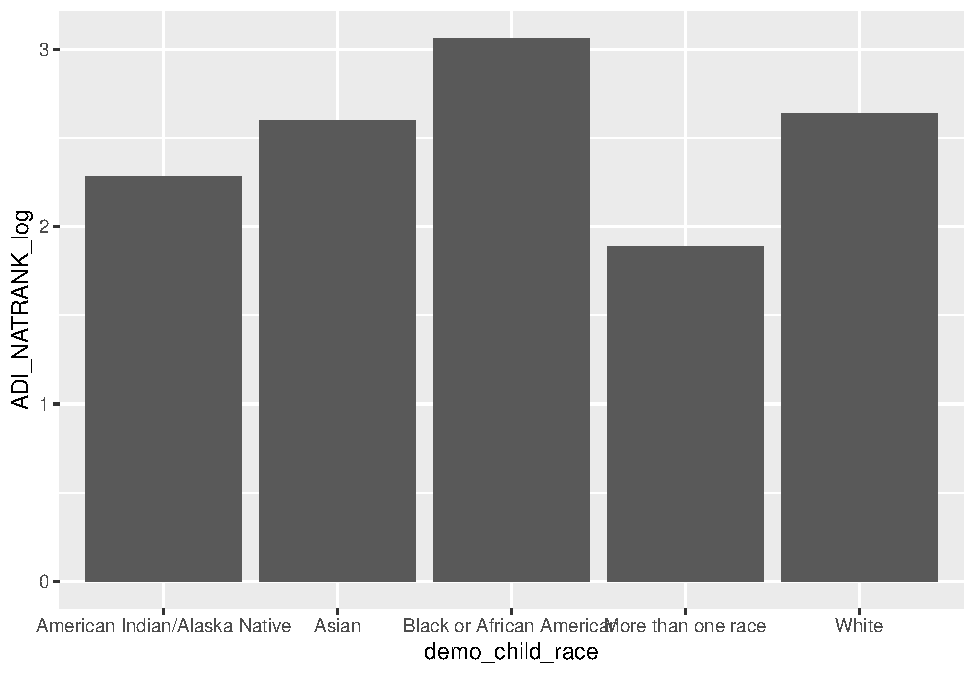
\includegraphics{do01_BUDS_files/figure-latex/unnamed-chunk-8-1.pdf}

\begin{Shaded}
\begin{Highlighting}[]
\FunctionTok{ggplot}\NormalTok{(df\_250450\_fz, }\FunctionTok{aes}\NormalTok{(}\AttributeTok{x=}\NormalTok{Racial\_majority, }\AttributeTok{y=}\NormalTok{ADI\_NATRANK\_log)) }\SpecialCharTok{+}
  \FunctionTok{geom\_bar}\NormalTok{(}\AttributeTok{stat =} \StringTok{"summary"}\NormalTok{, }\AttributeTok{fun.y =} \StringTok{"median"}\NormalTok{)}
\end{Highlighting}
\end{Shaded}

\begin{verbatim}
## Warning in geom_bar(stat = "summary", fun.y = "median"): Ignoring unknown
## parameters: `fun.y`
\end{verbatim}

\begin{verbatim}
## Warning: Removed 48 rows containing non-finite values (`stat_summary()`).
\end{verbatim}

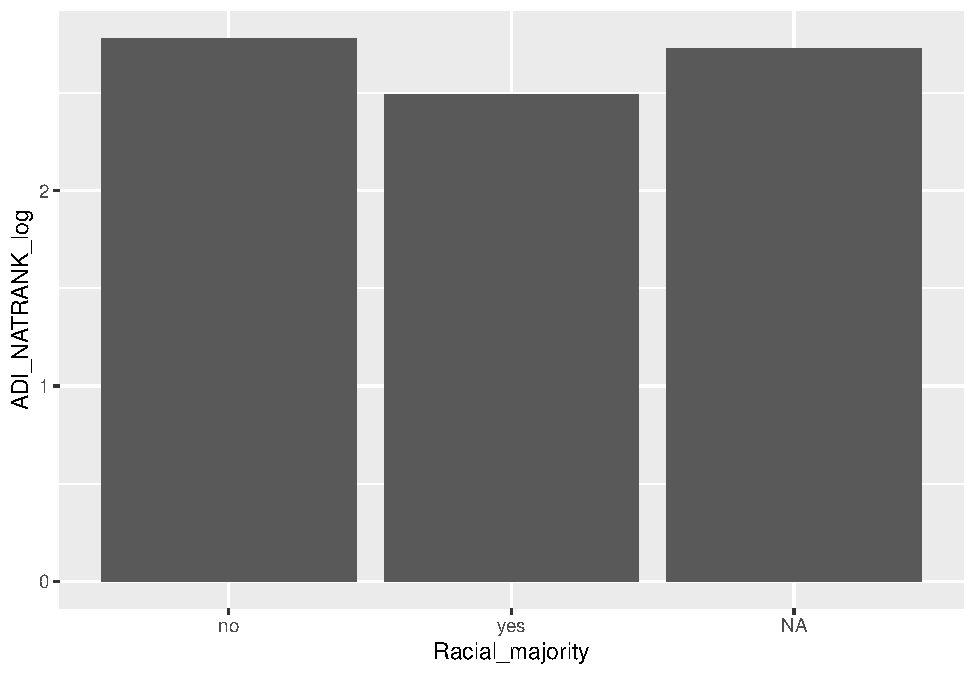
\includegraphics{do01_BUDS_files/figure-latex/unnamed-chunk-8-2.pdf}

\begin{Shaded}
\begin{Highlighting}[]
\FunctionTok{ggplot}\NormalTok{(df\_250450\_fz, }\FunctionTok{aes}\NormalTok{(}\AttributeTok{x=}\NormalTok{Racial\_minority, }\AttributeTok{y=}\NormalTok{ADI\_NATRANK\_log)) }\SpecialCharTok{+}
  \FunctionTok{geom\_bar}\NormalTok{(}\AttributeTok{stat =} \StringTok{"summary"}\NormalTok{, }\AttributeTok{fun.y =} \StringTok{"median"}\NormalTok{)}
\end{Highlighting}
\end{Shaded}

\begin{verbatim}
## Warning in geom_bar(stat = "summary", fun.y = "median"): Ignoring unknown parameters: `fun.y`
## Removed 48 rows containing non-finite values (`stat_summary()`).
\end{verbatim}

\includegraphics{do01_BUDS_files/figure-latex/unnamed-chunk-8-3.pdf}

\begin{Shaded}
\begin{Highlighting}[]
\FunctionTok{ggplot}\NormalTok{(df\_250450\_fz, }\FunctionTok{aes}\NormalTok{(}\AttributeTok{x=}\NormalTok{demo\_child\_hispanic, }\AttributeTok{y=}\NormalTok{ADI\_NATRANK\_log)) }\SpecialCharTok{+}
  \FunctionTok{geom\_bar}\NormalTok{(}\AttributeTok{stat =} \StringTok{"summary"}\NormalTok{, }\AttributeTok{fun.y =} \StringTok{"median"}\NormalTok{)}
\end{Highlighting}
\end{Shaded}

\begin{verbatim}
## Warning in geom_bar(stat = "summary", fun.y = "median"): Ignoring unknown parameters: `fun.y`
## Removed 48 rows containing non-finite values (`stat_summary()`).
\end{verbatim}

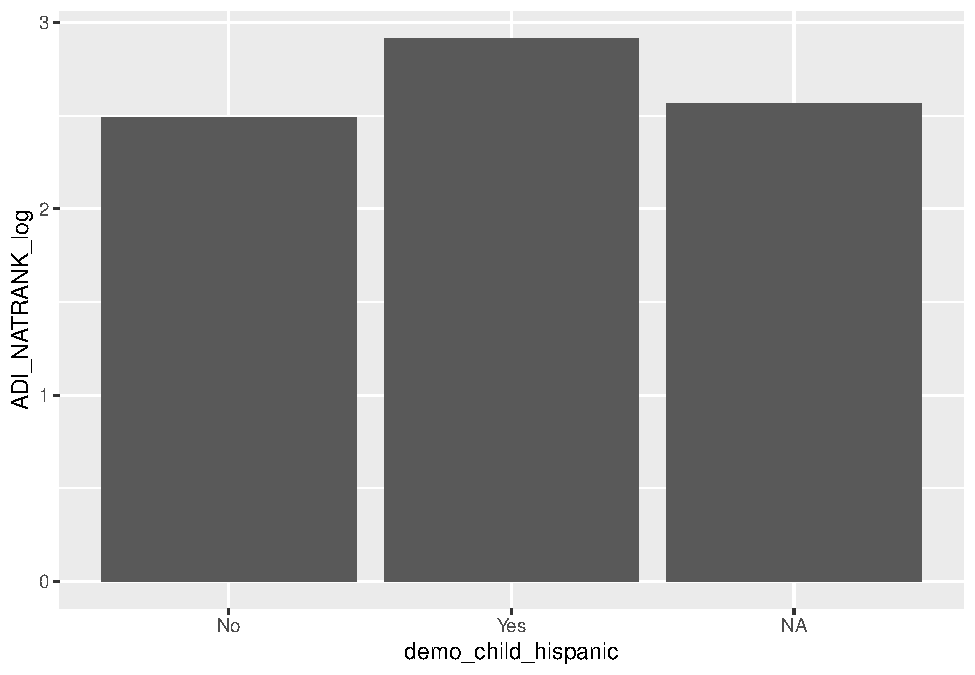
\includegraphics{do01_BUDS_files/figure-latex/unnamed-chunk-8-4.pdf}

\hypertarget{plots}{%
\subsection{Plots}\label{plots}}

\hypertarget{grand-average}{%
\subsubsection{Grand average}\label{grand-average}}

\begin{Shaded}
\begin{Highlighting}[]
\FunctionTok{ggplot}\NormalTok{(}\AttributeTok{data=}\FunctionTok{filter}\NormalTok{(df\_ga\_Cz\_adi\_wide, Condition}\SpecialCharTok{==}\StringTok{"Acc\_Acc"} \SpecialCharTok{|}\NormalTok{ Condition}\SpecialCharTok{==}\StringTok{"Acc\_Rej"} \SpecialCharTok{|}\NormalTok{ Condition}\SpecialCharTok{==}\StringTok{"AA\_AR"}\NormalTok{), }\FunctionTok{aes}\NormalTok{(}\AttributeTok{x=}\NormalTok{Time, }\AttributeTok{y=}\NormalTok{grand\_average, }\AttributeTok{color=}\NormalTok{Condition)) }\SpecialCharTok{+}
  \FunctionTok{facet\_wrap}\NormalTok{(}\SpecialCharTok{\textasciitilde{}}\NormalTok{ adi\_median\_split) }\SpecialCharTok{+}
  \FunctionTok{xlim}\NormalTok{(}\SpecialCharTok{{-}}\DecValTok{200}\NormalTok{, }\DecValTok{1000}\NormalTok{) }\SpecialCharTok{+}
  \FunctionTok{ylim}\NormalTok{( }\SpecialCharTok{{-}}\DecValTok{5}\NormalTok{, }\DecValTok{13}\NormalTok{) }\SpecialCharTok{+}
  \FunctionTok{geom\_line}\NormalTok{(}\AttributeTok{linewidth=}\DecValTok{1}\NormalTok{) }\SpecialCharTok{+}
  \FunctionTok{annotate}\NormalTok{(}\StringTok{"rect"}\NormalTok{, }\AttributeTok{xmin=}\DecValTok{150}\NormalTok{, }\AttributeTok{xmax=}\DecValTok{275}\NormalTok{, }\AttributeTok{ymin=}\DecValTok{0}\NormalTok{, }\AttributeTok{ymax=}\ConstantTok{Inf}\NormalTok{, }\AttributeTok{alpha=}\FloatTok{0.2}\NormalTok{, }\AttributeTok{fill=}\StringTok{"blue"}\NormalTok{) }\SpecialCharTok{+}
  \FunctionTok{geom\_rect}\NormalTok{(}\FunctionTok{aes}\NormalTok{(}\AttributeTok{xmin=}\DecValTok{0}\NormalTok{, }\AttributeTok{xmax=}\DecValTok{0}\NormalTok{, }\AttributeTok{ymin=}\SpecialCharTok{{-}}\DecValTok{5}\NormalTok{, }\AttributeTok{ymax=}\DecValTok{12}\NormalTok{), }\AttributeTok{color=}\StringTok{"black"}\NormalTok{) }\SpecialCharTok{+}
  \FunctionTok{geom\_rect}\NormalTok{(}\FunctionTok{aes}\NormalTok{(}\AttributeTok{xmin=}\SpecialCharTok{{-}}\DecValTok{200}\NormalTok{, }\AttributeTok{xmax=}\DecValTok{800}\NormalTok{, }\AttributeTok{ymin=}\DecValTok{0}\NormalTok{, }\AttributeTok{ymax=}\DecValTok{0}\NormalTok{), }\AttributeTok{color=}\StringTok{"black"}\NormalTok{) }\SpecialCharTok{+}
  \FunctionTok{scale\_color\_manual}\NormalTok{(}\AttributeTok{breaks=}\FunctionTok{c}\NormalTok{(}\StringTok{"Acc\_Acc"}\NormalTok{,}\StringTok{"Acc\_Rej"}\NormalTok{,}\StringTok{"AA\_AR"}\NormalTok{),}
                     \AttributeTok{values=}\FunctionTok{c}\NormalTok{(}\StringTok{"Acc\_Acc"}\OtherTok{=}\StringTok{"green"}\NormalTok{, }\StringTok{"AA\_AR"}\OtherTok{=}\StringTok{"black"}\NormalTok{, }\StringTok{"Acc\_Rej"}\OtherTok{=}\StringTok{"red"}\NormalTok{), }
                     \AttributeTok{labels=}\FunctionTok{c}\NormalTok{(}\StringTok{"Acceptance"}\NormalTok{,}\StringTok{"Rejection"}\NormalTok{,}\StringTok{"Difference"}\NormalTok{), }\AttributeTok{name=}\ConstantTok{NULL}\NormalTok{) }\SpecialCharTok{+}
  \FunctionTok{labs}\NormalTok{(}\AttributeTok{x=}\StringTok{"Time (ms)"}\NormalTok{, }\AttributeTok{y=}\StringTok{"Cz"}\NormalTok{, }\AttributeTok{title=}\StringTok{"High value peers"}\NormalTok{) }\SpecialCharTok{+}
  \FunctionTok{theme\_apa}\NormalTok{(}\AttributeTok{base\_size =} \DecValTok{12}\NormalTok{) }\SpecialCharTok{+} \FunctionTok{theme}\NormalTok{(}\AttributeTok{legend.position=}\StringTok{"top"}\NormalTok{)}
\end{Highlighting}
\end{Shaded}

\begin{verbatim}
## Warning: Removed 1497 rows containing missing values (`geom_line()`).
\end{verbatim}

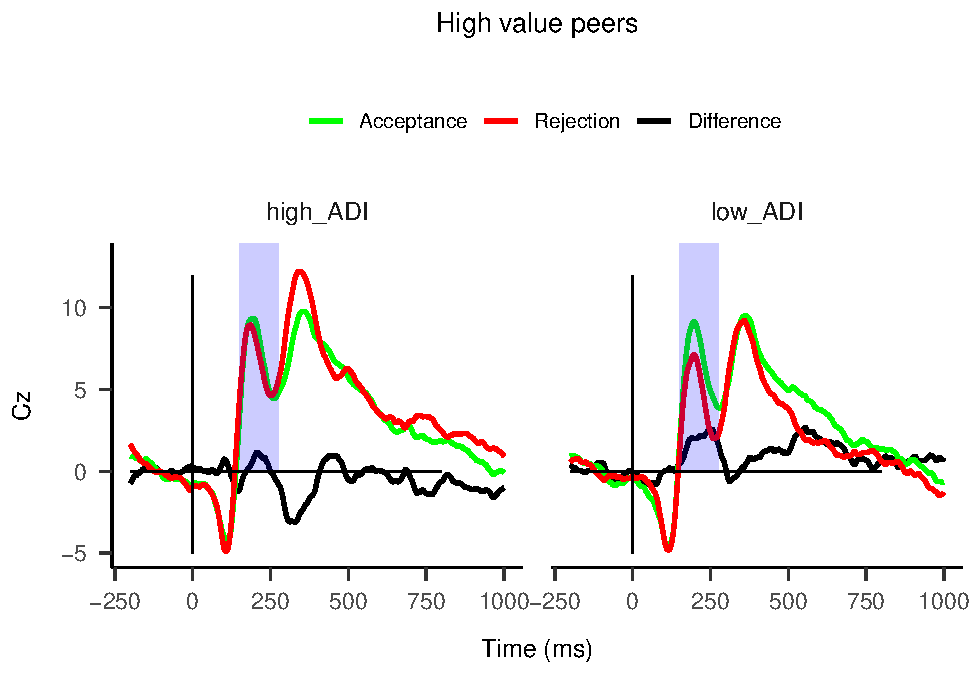
\includegraphics{do01_BUDS_files/figure-latex/unnamed-chunk-9-1.pdf}

\begin{Shaded}
\begin{Highlighting}[]
\FunctionTok{ggplot}\NormalTok{(}\AttributeTok{data=}\FunctionTok{filter}\NormalTok{(df\_ga\_Cz\_adi\_wide, Condition}\SpecialCharTok{==}\StringTok{"Acc\_Acc"} \SpecialCharTok{|}\NormalTok{ Condition}\SpecialCharTok{==}\StringTok{"Acc\_Rej"} \SpecialCharTok{|}\NormalTok{ Condition}\SpecialCharTok{==}\StringTok{"AA\_AR"}\NormalTok{), }\FunctionTok{aes}\NormalTok{(}\AttributeTok{x=}\NormalTok{Time, }\AttributeTok{y=}\NormalTok{grand\_average, }\AttributeTok{color=}\NormalTok{Condition)) }\SpecialCharTok{+}
  \FunctionTok{facet\_wrap}\NormalTok{(}\SpecialCharTok{\textasciitilde{}}\NormalTok{ adi\_median\_split) }\SpecialCharTok{+}
  \FunctionTok{xlim}\NormalTok{(}\SpecialCharTok{{-}}\DecValTok{200}\NormalTok{, }\DecValTok{1000}\NormalTok{) }\SpecialCharTok{+}
  \FunctionTok{ylim}\NormalTok{( }\SpecialCharTok{{-}}\DecValTok{5}\NormalTok{, }\DecValTok{13}\NormalTok{) }\SpecialCharTok{+}
  \FunctionTok{geom\_line}\NormalTok{(}\AttributeTok{linewidth=}\DecValTok{1}\NormalTok{) }\SpecialCharTok{+}
  \FunctionTok{annotate}\NormalTok{(}\StringTok{"rect"}\NormalTok{, }\AttributeTok{xmin=}\DecValTok{275}\NormalTok{, }\AttributeTok{xmax=}\DecValTok{425}\NormalTok{, }\AttributeTok{ymin=}\DecValTok{0}\NormalTok{, }\AttributeTok{ymax=}\ConstantTok{Inf}\NormalTok{, }\AttributeTok{alpha=}\FloatTok{0.2}\NormalTok{, }\AttributeTok{fill=}\StringTok{"blue"}\NormalTok{) }\SpecialCharTok{+}
  \FunctionTok{geom\_rect}\NormalTok{(}\FunctionTok{aes}\NormalTok{(}\AttributeTok{xmin=}\DecValTok{0}\NormalTok{, }\AttributeTok{xmax=}\DecValTok{0}\NormalTok{, }\AttributeTok{ymin=}\SpecialCharTok{{-}}\DecValTok{5}\NormalTok{, }\AttributeTok{ymax=}\DecValTok{12}\NormalTok{), }\AttributeTok{color=}\StringTok{"black"}\NormalTok{) }\SpecialCharTok{+}
  \FunctionTok{geom\_rect}\NormalTok{(}\FunctionTok{aes}\NormalTok{(}\AttributeTok{xmin=}\SpecialCharTok{{-}}\DecValTok{200}\NormalTok{, }\AttributeTok{xmax=}\DecValTok{800}\NormalTok{, }\AttributeTok{ymin=}\DecValTok{0}\NormalTok{, }\AttributeTok{ymax=}\DecValTok{0}\NormalTok{), }\AttributeTok{color=}\StringTok{"black"}\NormalTok{) }\SpecialCharTok{+}
  \FunctionTok{scale\_color\_manual}\NormalTok{(}\AttributeTok{breaks=}\FunctionTok{c}\NormalTok{(}\StringTok{"Acc\_Acc"}\NormalTok{,}\StringTok{"Acc\_Rej"}\NormalTok{,}\StringTok{"AA\_AR"}\NormalTok{),}
                     \AttributeTok{values=}\FunctionTok{c}\NormalTok{(}\StringTok{"Acc\_Acc"}\OtherTok{=}\StringTok{"green"}\NormalTok{, }\StringTok{"AA\_AR"}\OtherTok{=}\StringTok{"black"}\NormalTok{, }\StringTok{"Acc\_Rej"}\OtherTok{=}\StringTok{"red"}\NormalTok{), }
                     \AttributeTok{labels=}\FunctionTok{c}\NormalTok{(}\StringTok{"Acceptance"}\NormalTok{,}\StringTok{"Rejection"}\NormalTok{,}\StringTok{"Difference"}\NormalTok{), }\AttributeTok{name=}\ConstantTok{NULL}\NormalTok{) }\SpecialCharTok{+}
  \FunctionTok{labs}\NormalTok{(}\AttributeTok{x=}\StringTok{"Time (ms)"}\NormalTok{, }\AttributeTok{y=}\StringTok{"Cz"}\NormalTok{, }\AttributeTok{title=}\StringTok{"High value peers"}\NormalTok{) }\SpecialCharTok{+}
  \FunctionTok{theme\_apa}\NormalTok{(}\AttributeTok{base\_size =} \DecValTok{12}\NormalTok{) }\SpecialCharTok{+} \FunctionTok{theme}\NormalTok{(}\AttributeTok{legend.position=}\StringTok{"top"}\NormalTok{)}
\end{Highlighting}
\end{Shaded}

\begin{verbatim}
## Warning: Removed 1497 rows containing missing values (`geom_line()`).
\end{verbatim}

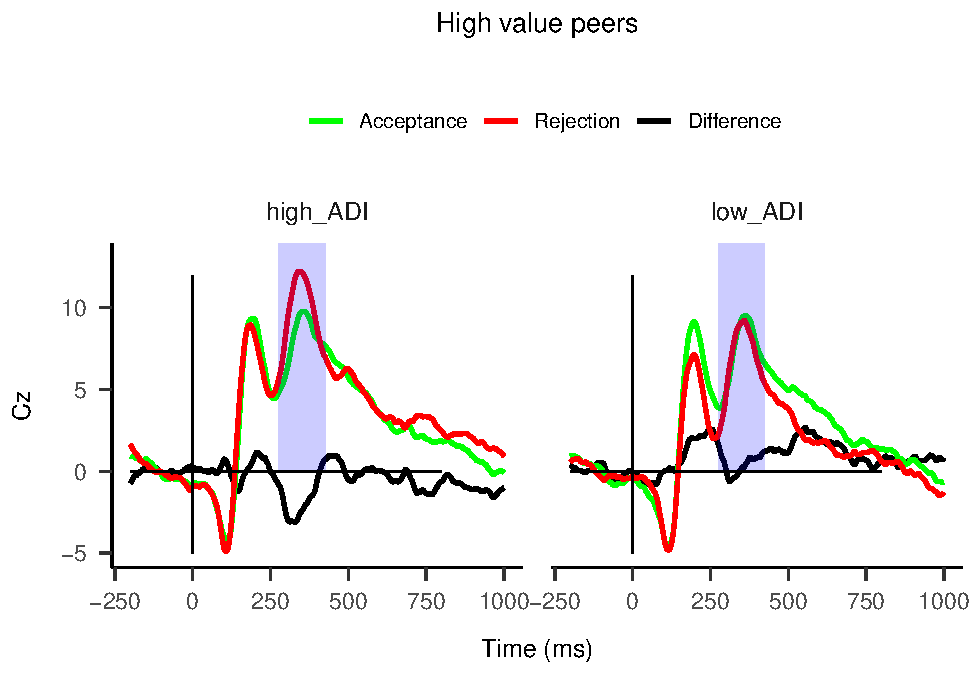
\includegraphics{do01_BUDS_files/figure-latex/unnamed-chunk-9-2.pdf}

\begin{Shaded}
\begin{Highlighting}[]
\FunctionTok{ggplot}\NormalTok{(}\AttributeTok{data=}\FunctionTok{filter}\NormalTok{(df\_ga\_Cz\_adi\_wide, Condition}\SpecialCharTok{==}\StringTok{"Rej\_Acc"} \SpecialCharTok{|}\NormalTok{ Condition}\SpecialCharTok{==}\StringTok{"Rej\_Rej"} \SpecialCharTok{|}\NormalTok{ Condition}\SpecialCharTok{==}\StringTok{"RA\_RR"}\NormalTok{), }\FunctionTok{aes}\NormalTok{(}\AttributeTok{x=}\NormalTok{Time, }\AttributeTok{y=}\NormalTok{grand\_average, }\AttributeTok{color=}\NormalTok{Condition)) }\SpecialCharTok{+}
  \FunctionTok{facet\_wrap}\NormalTok{(}\SpecialCharTok{\textasciitilde{}}\NormalTok{ adi\_median\_split) }\SpecialCharTok{+}
  \FunctionTok{xlim}\NormalTok{(}\SpecialCharTok{{-}}\DecValTok{200}\NormalTok{, }\DecValTok{800}\NormalTok{) }\SpecialCharTok{+}
  \FunctionTok{ylim}\NormalTok{( }\SpecialCharTok{{-}}\DecValTok{5}\NormalTok{, }\DecValTok{13}\NormalTok{) }\SpecialCharTok{+}
  \FunctionTok{geom\_line}\NormalTok{(}\AttributeTok{linewidth=}\DecValTok{1}\NormalTok{) }\SpecialCharTok{+}
  \FunctionTok{annotate}\NormalTok{(}\StringTok{"rect"}\NormalTok{, }\AttributeTok{xmin=}\DecValTok{150}\NormalTok{, }\AttributeTok{xmax=}\DecValTok{350}\NormalTok{, }\AttributeTok{ymin=}\DecValTok{0}\NormalTok{, }\AttributeTok{ymax=}\ConstantTok{Inf}\NormalTok{, }\AttributeTok{alpha=}\FloatTok{0.2}\NormalTok{, }\AttributeTok{fill=}\StringTok{"blue"}\NormalTok{) }\SpecialCharTok{+}
  \FunctionTok{geom\_rect}\NormalTok{(}\FunctionTok{aes}\NormalTok{(}\AttributeTok{xmin=}\DecValTok{0}\NormalTok{, }\AttributeTok{xmax=}\DecValTok{0}\NormalTok{, }\AttributeTok{ymin=}\SpecialCharTok{{-}}\DecValTok{5}\NormalTok{, }\AttributeTok{ymax=}\DecValTok{12}\NormalTok{), }\AttributeTok{color=}\StringTok{"black"}\NormalTok{) }\SpecialCharTok{+}
  \FunctionTok{geom\_rect}\NormalTok{(}\FunctionTok{aes}\NormalTok{(}\AttributeTok{xmin=}\SpecialCharTok{{-}}\DecValTok{200}\NormalTok{, }\AttributeTok{xmax=}\DecValTok{800}\NormalTok{, }\AttributeTok{ymin=}\DecValTok{0}\NormalTok{, }\AttributeTok{ymax=}\DecValTok{0}\NormalTok{), }\AttributeTok{color=}\StringTok{"black"}\NormalTok{) }\SpecialCharTok{+}
  \FunctionTok{scale\_color\_manual}\NormalTok{(}\AttributeTok{breaks=}\FunctionTok{c}\NormalTok{(}\StringTok{"Rej\_Acc"}\NormalTok{,}\StringTok{"Rej\_Rej"}\NormalTok{,}\StringTok{"RA\_RR"}\NormalTok{),}
                     \AttributeTok{values=}\FunctionTok{c}\NormalTok{(}\StringTok{"Rej\_Acc"}\OtherTok{=}\StringTok{"green"}\NormalTok{, }\StringTok{"RA\_RR"}\OtherTok{=}\StringTok{"black"}\NormalTok{, }\StringTok{"Rej\_Rej"}\OtherTok{=}\StringTok{"red"}\NormalTok{), }
                     \AttributeTok{labels=}\FunctionTok{c}\NormalTok{(}\StringTok{"Acceptance"}\NormalTok{,}\StringTok{"Rejection"}\NormalTok{,}\StringTok{"Difference"}\NormalTok{), }\AttributeTok{name=}\ConstantTok{NULL}\NormalTok{) }\SpecialCharTok{+}
  \FunctionTok{labs}\NormalTok{(}\AttributeTok{x=}\StringTok{"Time (ms)"}\NormalTok{, }\AttributeTok{y=}\StringTok{"Cz"}\NormalTok{, }\AttributeTok{title=}\StringTok{"Low value peers"}\NormalTok{) }\SpecialCharTok{+}
  \FunctionTok{theme\_apa}\NormalTok{(}\AttributeTok{base\_size =} \DecValTok{12}\NormalTok{) }\SpecialCharTok{+} \FunctionTok{theme}\NormalTok{(}\AttributeTok{legend.position=}\StringTok{"top"}\NormalTok{)}
\end{Highlighting}
\end{Shaded}

\begin{verbatim}
## Warning: Removed 1797 rows containing missing values (`geom_line()`).
\end{verbatim}

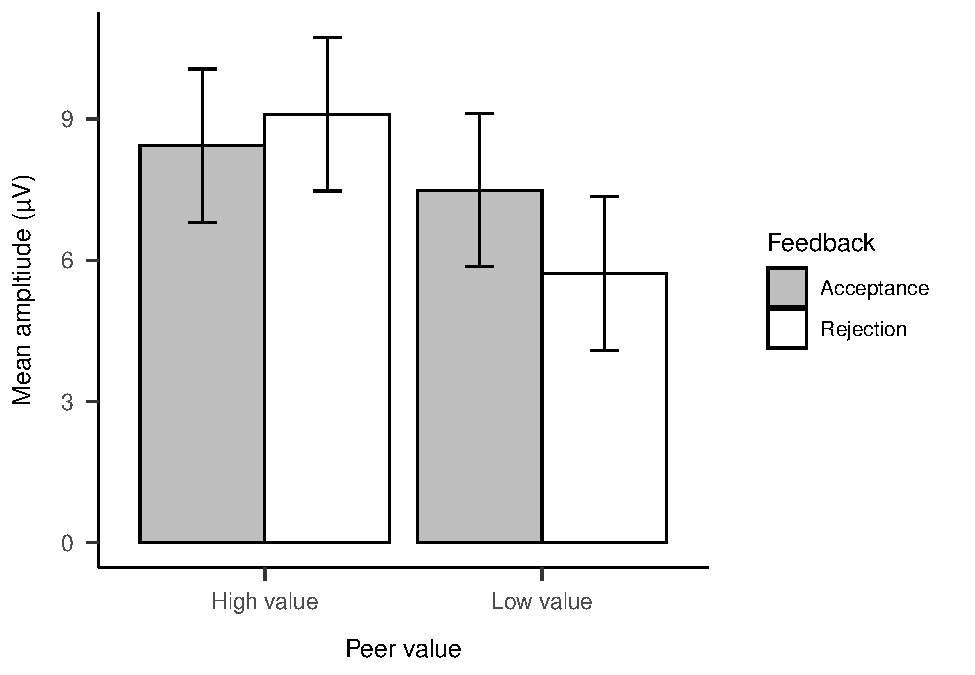
\includegraphics{do01_BUDS_files/figure-latex/unnamed-chunk-9-3.pdf}

\begin{Shaded}
\begin{Highlighting}[]
\FunctionTok{ggplot}\NormalTok{(}\AttributeTok{data=}\FunctionTok{filter}\NormalTok{(df\_ga\_Fz\_adi\_wide, Condition}\SpecialCharTok{==}\StringTok{"Acc\_Acc"} \SpecialCharTok{|}\NormalTok{ Condition}\SpecialCharTok{==}\StringTok{"Acc\_Rej"} \SpecialCharTok{|}\NormalTok{ Condition}\SpecialCharTok{==}\StringTok{"AA\_AR"}\NormalTok{), }\FunctionTok{aes}\NormalTok{(}\AttributeTok{x=}\NormalTok{Time, }\AttributeTok{y=}\NormalTok{grand\_average, }\AttributeTok{color=}\NormalTok{Condition)) }\SpecialCharTok{+}
  \FunctionTok{facet\_wrap}\NormalTok{(}\SpecialCharTok{\textasciitilde{}}\NormalTok{ adi\_median\_split) }\SpecialCharTok{+}
  \FunctionTok{xlim}\NormalTok{(}\SpecialCharTok{{-}}\DecValTok{200}\NormalTok{, }\DecValTok{800}\NormalTok{) }\SpecialCharTok{+}
  \FunctionTok{geom\_line}\NormalTok{(}\AttributeTok{linewidth=}\DecValTok{1}\NormalTok{) }\SpecialCharTok{+}
  \FunctionTok{annotate}\NormalTok{(}\StringTok{"rect"}\NormalTok{, }\AttributeTok{xmin=}\DecValTok{100}\NormalTok{, }\AttributeTok{xmax=}\DecValTok{450}\NormalTok{, }\AttributeTok{ymin=}\DecValTok{0}\NormalTok{, }\AttributeTok{ymax=}\ConstantTok{Inf}\NormalTok{, }\AttributeTok{alpha=}\FloatTok{0.2}\NormalTok{, }\AttributeTok{fill=}\StringTok{"blue"}\NormalTok{) }\SpecialCharTok{+}
  \FunctionTok{geom\_rect}\NormalTok{(}\FunctionTok{aes}\NormalTok{(}\AttributeTok{xmin=}\DecValTok{0}\NormalTok{, }\AttributeTok{xmax=}\DecValTok{0}\NormalTok{, }\AttributeTok{ymin=}\SpecialCharTok{{-}}\DecValTok{5}\NormalTok{, }\AttributeTok{ymax=}\DecValTok{10}\NormalTok{), }\AttributeTok{color=}\StringTok{"black"}\NormalTok{) }\SpecialCharTok{+}
  \FunctionTok{geom\_rect}\NormalTok{(}\FunctionTok{aes}\NormalTok{(}\AttributeTok{xmin=}\SpecialCharTok{{-}}\DecValTok{200}\NormalTok{, }\AttributeTok{xmax=}\DecValTok{800}\NormalTok{, }\AttributeTok{ymin=}\DecValTok{0}\NormalTok{, }\AttributeTok{ymax=}\DecValTok{0}\NormalTok{), }\AttributeTok{color=}\StringTok{"black"}\NormalTok{) }\SpecialCharTok{+}
  \FunctionTok{scale\_color\_manual}\NormalTok{(}\AttributeTok{breaks=}\FunctionTok{c}\NormalTok{(}\StringTok{"Acc\_Acc"}\NormalTok{,}\StringTok{"Acc\_Rej"}\NormalTok{,}\StringTok{"AA\_AR"}\NormalTok{),}
                     \AttributeTok{values=}\FunctionTok{c}\NormalTok{(}\StringTok{"Acc\_Acc"}\OtherTok{=}\StringTok{"green"}\NormalTok{, }\StringTok{"AA\_AR"}\OtherTok{=}\StringTok{"black"}\NormalTok{, }\StringTok{"Acc\_Rej"}\OtherTok{=}\StringTok{"red"}\NormalTok{), }
                     \AttributeTok{labels=}\FunctionTok{c}\NormalTok{(}\StringTok{"Acceptance"}\NormalTok{,}\StringTok{"Rejection"}\NormalTok{,}\StringTok{"Difference"}\NormalTok{), }\AttributeTok{name=}\ConstantTok{NULL}\NormalTok{) }\SpecialCharTok{+}
  \FunctionTok{labs}\NormalTok{(}\AttributeTok{x=}\StringTok{"Time (ms)"}\NormalTok{, }\AttributeTok{y=}\StringTok{"Fz"}\NormalTok{, }\AttributeTok{title=}\StringTok{"High value peers"}\NormalTok{) }\SpecialCharTok{+}
  \FunctionTok{theme\_apa}\NormalTok{(}\AttributeTok{base\_size =} \DecValTok{12}\NormalTok{) }\SpecialCharTok{+} \FunctionTok{theme}\NormalTok{(}\AttributeTok{legend.position=}\StringTok{"top"}\NormalTok{)}
\end{Highlighting}
\end{Shaded}

\begin{verbatim}
## Warning: Removed 1797 rows containing missing values (`geom_line()`).
\end{verbatim}

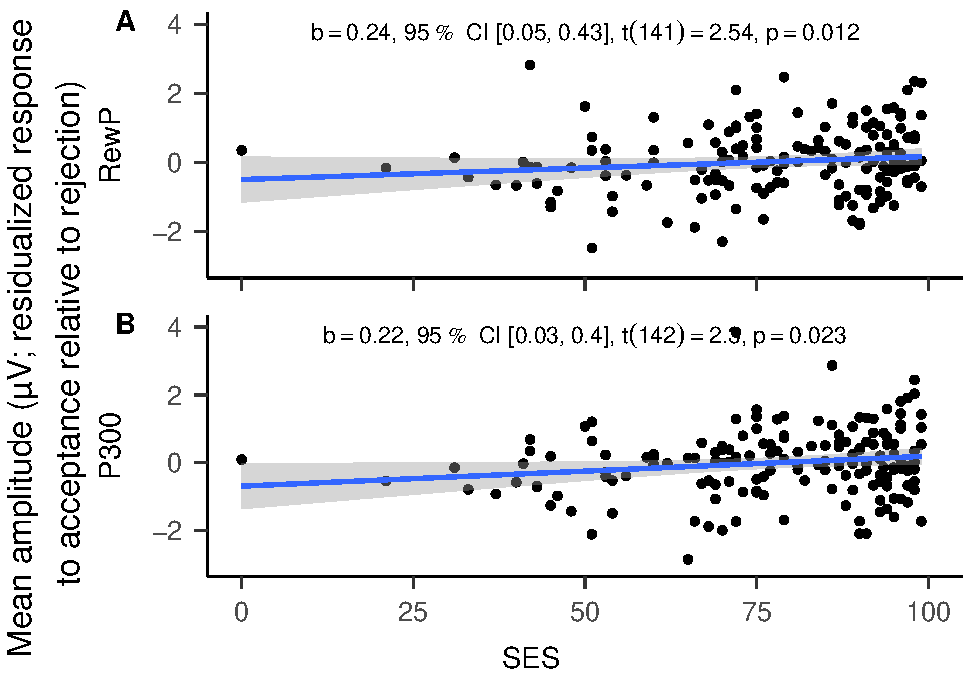
\includegraphics{do01_BUDS_files/figure-latex/unnamed-chunk-10-1.pdf}

\begin{Shaded}
\begin{Highlighting}[]
\FunctionTok{ggplot}\NormalTok{(}\AttributeTok{data=}\FunctionTok{filter}\NormalTok{(df\_ga\_Fz\_adi\_wide, Condition}\SpecialCharTok{==}\StringTok{"Rej\_Acc"} \SpecialCharTok{|}\NormalTok{ Condition}\SpecialCharTok{==}\StringTok{"Rej\_Rej"} \SpecialCharTok{|}\NormalTok{ Condition}\SpecialCharTok{==}\StringTok{"RA\_RR"}\NormalTok{), }\FunctionTok{aes}\NormalTok{(}\AttributeTok{x=}\NormalTok{Time, }\AttributeTok{y=}\NormalTok{grand\_average, }\AttributeTok{color=}\NormalTok{Condition)) }\SpecialCharTok{+}
  \FunctionTok{facet\_wrap}\NormalTok{(}\SpecialCharTok{\textasciitilde{}}\NormalTok{ adi\_median\_split) }\SpecialCharTok{+}
  \FunctionTok{xlim}\NormalTok{(}\SpecialCharTok{{-}}\DecValTok{200}\NormalTok{, }\DecValTok{800}\NormalTok{) }\SpecialCharTok{+}
  \FunctionTok{geom\_line}\NormalTok{(}\AttributeTok{linewidth=}\DecValTok{1}\NormalTok{) }\SpecialCharTok{+}
  \FunctionTok{annotate}\NormalTok{(}\StringTok{"rect"}\NormalTok{, }\AttributeTok{xmin=}\DecValTok{250}\NormalTok{, }\AttributeTok{xmax=}\DecValTok{450}\NormalTok{, }\AttributeTok{ymin=}\DecValTok{0}\NormalTok{, }\AttributeTok{ymax=}\ConstantTok{Inf}\NormalTok{, }\AttributeTok{alpha=}\FloatTok{0.2}\NormalTok{, }\AttributeTok{fill=}\StringTok{"blue"}\NormalTok{) }\SpecialCharTok{+}
  \FunctionTok{geom\_rect}\NormalTok{(}\FunctionTok{aes}\NormalTok{(}\AttributeTok{xmin=}\DecValTok{0}\NormalTok{, }\AttributeTok{xmax=}\DecValTok{0}\NormalTok{, }\AttributeTok{ymin=}\SpecialCharTok{{-}}\DecValTok{5}\NormalTok{, }\AttributeTok{ymax=}\DecValTok{10}\NormalTok{), }\AttributeTok{color=}\StringTok{"black"}\NormalTok{) }\SpecialCharTok{+}
  \FunctionTok{geom\_rect}\NormalTok{(}\FunctionTok{aes}\NormalTok{(}\AttributeTok{xmin=}\SpecialCharTok{{-}}\DecValTok{200}\NormalTok{, }\AttributeTok{xmax=}\DecValTok{800}\NormalTok{, }\AttributeTok{ymin=}\DecValTok{0}\NormalTok{, }\AttributeTok{ymax=}\DecValTok{0}\NormalTok{), }\AttributeTok{color=}\StringTok{"black"}\NormalTok{) }\SpecialCharTok{+}
  \FunctionTok{scale\_color\_manual}\NormalTok{(}\AttributeTok{breaks=}\FunctionTok{c}\NormalTok{(}\StringTok{"Rej\_Acc"}\NormalTok{,}\StringTok{"Rej\_Rej"}\NormalTok{,}\StringTok{"RA\_RR"}\NormalTok{),}
                     \AttributeTok{values=}\FunctionTok{c}\NormalTok{(}\StringTok{"Rej\_Acc"}\OtherTok{=}\StringTok{"green"}\NormalTok{, }\StringTok{"RA\_RR"}\OtherTok{=}\StringTok{"black"}\NormalTok{, }\StringTok{"Rej\_Rej"}\OtherTok{=}\StringTok{"red"}\NormalTok{), }
                     \AttributeTok{labels=}\FunctionTok{c}\NormalTok{(}\StringTok{"Acceptance"}\NormalTok{,}\StringTok{"Rejection"}\NormalTok{,}\StringTok{"Difference"}\NormalTok{), }\AttributeTok{name=}\ConstantTok{NULL}\NormalTok{) }\SpecialCharTok{+}
  \FunctionTok{labs}\NormalTok{(}\AttributeTok{x=}\StringTok{"Time (ms)"}\NormalTok{, }\AttributeTok{y=}\StringTok{"Fz"}\NormalTok{, }\AttributeTok{title=}\StringTok{"Low value peers"}\NormalTok{) }\SpecialCharTok{+}
  \FunctionTok{theme\_apa}\NormalTok{(}\AttributeTok{base\_size =} \DecValTok{12}\NormalTok{) }\SpecialCharTok{+} \FunctionTok{theme}\NormalTok{(}\AttributeTok{legend.position=}\StringTok{"top"}\NormalTok{)}
\end{Highlighting}
\end{Shaded}

\begin{verbatim}
## Warning: Removed 1797 rows containing missing values (`geom_line()`).
\end{verbatim}

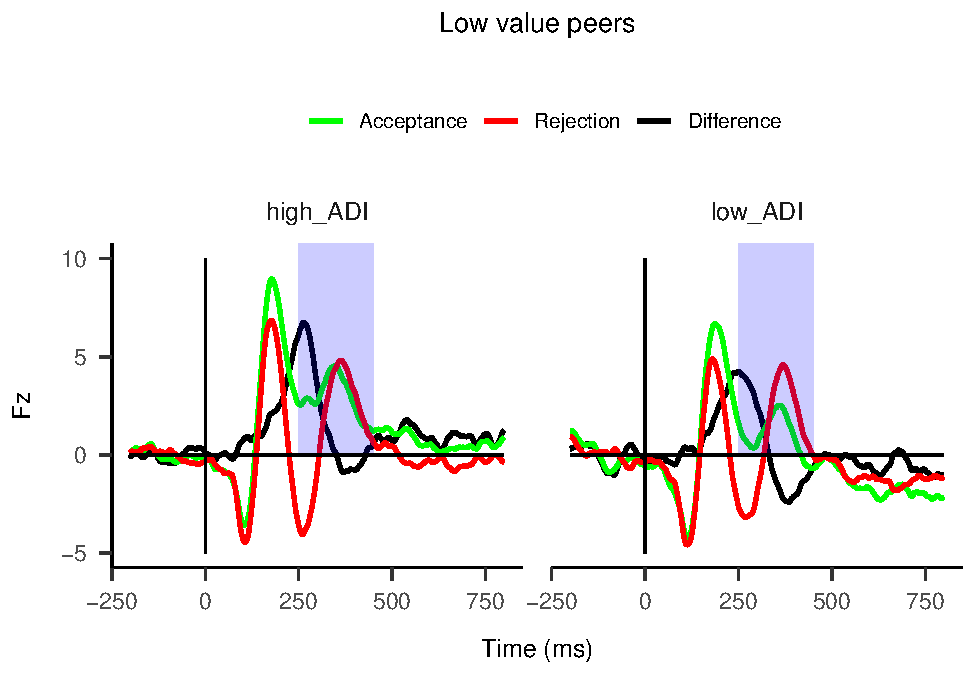
\includegraphics{do01_BUDS_files/figure-latex/unnamed-chunk-10-2.pdf}

\begin{Shaded}
\begin{Highlighting}[]
\FunctionTok{ggplot}\NormalTok{(}\AttributeTok{data=}\FunctionTok{filter}\NormalTok{(df\_ga\_Pz\_adi\_wide, Condition}\SpecialCharTok{==}\StringTok{"Acc\_Acc"} \SpecialCharTok{|}\NormalTok{ Condition}\SpecialCharTok{==}\StringTok{"Acc\_Rej"} \SpecialCharTok{|}\NormalTok{ Condition}\SpecialCharTok{==}\StringTok{"AA\_AR"}\NormalTok{), }\FunctionTok{aes}\NormalTok{(}\AttributeTok{x=}\NormalTok{Time, }\AttributeTok{y=}\NormalTok{grand\_average, }\AttributeTok{color=}\NormalTok{Condition)) }\SpecialCharTok{+}
  \FunctionTok{facet\_wrap}\NormalTok{(}\SpecialCharTok{\textasciitilde{}}\NormalTok{ adi\_median\_split) }\SpecialCharTok{+}
  \FunctionTok{xlim}\NormalTok{(}\SpecialCharTok{{-}}\DecValTok{200}\NormalTok{, }\DecValTok{1000}\NormalTok{) }\SpecialCharTok{+}
  \FunctionTok{geom\_line}\NormalTok{(}\AttributeTok{linewidth=}\DecValTok{1}\NormalTok{) }\SpecialCharTok{+}
  \FunctionTok{annotate}\NormalTok{(}\StringTok{"rect"}\NormalTok{, }\AttributeTok{xmin=}\DecValTok{275}\NormalTok{, }\AttributeTok{xmax=}\DecValTok{425}\NormalTok{, }\AttributeTok{ymin=}\DecValTok{0}\NormalTok{, }\AttributeTok{ymax=}\ConstantTok{Inf}\NormalTok{, }\AttributeTok{alpha=}\FloatTok{0.2}\NormalTok{, }\AttributeTok{fill=}\StringTok{"blue"}\NormalTok{) }\SpecialCharTok{+}
  \FunctionTok{geom\_rect}\NormalTok{(}\FunctionTok{aes}\NormalTok{(}\AttributeTok{xmin=}\DecValTok{0}\NormalTok{, }\AttributeTok{xmax=}\DecValTok{0}\NormalTok{, }\AttributeTok{ymin=}\SpecialCharTok{{-}}\DecValTok{5}\NormalTok{, }\AttributeTok{ymax=}\DecValTok{10}\NormalTok{), }\AttributeTok{color=}\StringTok{"black"}\NormalTok{) }\SpecialCharTok{+}
  \FunctionTok{geom\_rect}\NormalTok{(}\FunctionTok{aes}\NormalTok{(}\AttributeTok{xmin=}\SpecialCharTok{{-}}\DecValTok{200}\NormalTok{, }\AttributeTok{xmax=}\DecValTok{800}\NormalTok{, }\AttributeTok{ymin=}\DecValTok{0}\NormalTok{, }\AttributeTok{ymax=}\DecValTok{0}\NormalTok{), }\AttributeTok{color=}\StringTok{"black"}\NormalTok{) }\SpecialCharTok{+}
  \FunctionTok{scale\_color\_manual}\NormalTok{(}\AttributeTok{breaks=}\FunctionTok{c}\NormalTok{(}\StringTok{"Acc\_Acc"}\NormalTok{,}\StringTok{"Acc\_Rej"}\NormalTok{,}\StringTok{"AA\_AR"}\NormalTok{),}
                     \AttributeTok{values=}\FunctionTok{c}\NormalTok{(}\StringTok{"Acc\_Acc"}\OtherTok{=}\StringTok{"green"}\NormalTok{, }\StringTok{"AA\_AR"}\OtherTok{=}\StringTok{"black"}\NormalTok{, }\StringTok{"Acc\_Rej"}\OtherTok{=}\StringTok{"red"}\NormalTok{), }
                     \AttributeTok{labels=}\FunctionTok{c}\NormalTok{(}\StringTok{"Acceptance"}\NormalTok{,}\StringTok{"Rejection"}\NormalTok{,}\StringTok{"Difference"}\NormalTok{), }\AttributeTok{name=}\ConstantTok{NULL}\NormalTok{) }\SpecialCharTok{+}
  \FunctionTok{labs}\NormalTok{(}\AttributeTok{x=}\StringTok{"Time (ms)"}\NormalTok{, }\AttributeTok{y=}\StringTok{"Pz"}\NormalTok{, }\AttributeTok{title=}\StringTok{"High value peers"}\NormalTok{) }\SpecialCharTok{+}
  \FunctionTok{theme\_apa}\NormalTok{(}\AttributeTok{base\_size =} \DecValTok{12}\NormalTok{) }\SpecialCharTok{+} \FunctionTok{theme}\NormalTok{(}\AttributeTok{legend.position=}\StringTok{"top"}\NormalTok{)}
\end{Highlighting}
\end{Shaded}

\begin{verbatim}
## Warning: Removed 1497 rows containing missing values (`geom_line()`).
\end{verbatim}

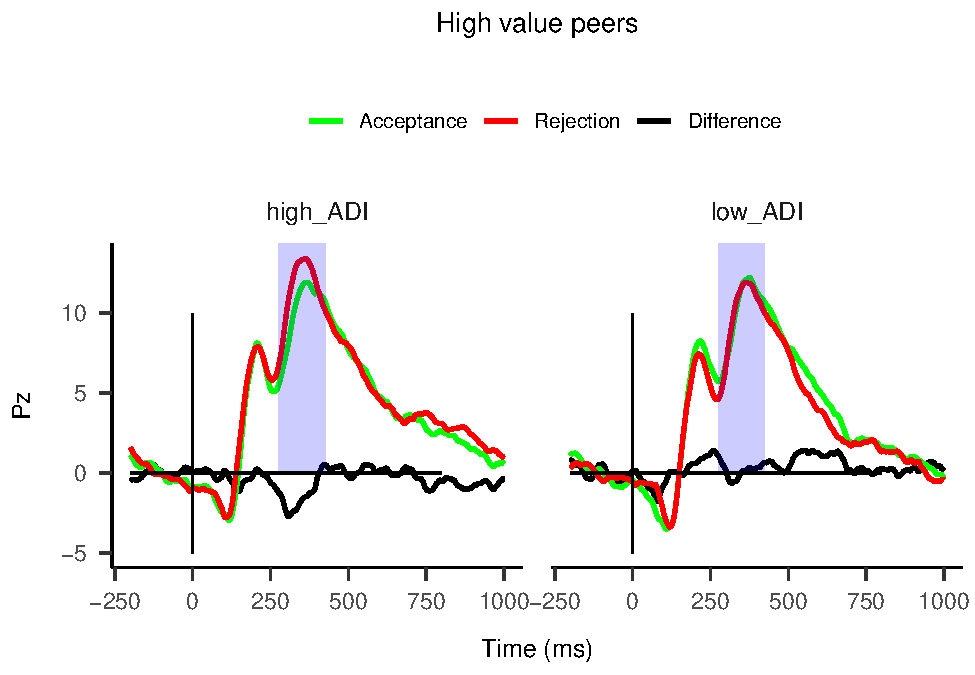
\includegraphics{do01_BUDS_files/figure-latex/unnamed-chunk-11-1.pdf}

\begin{Shaded}
\begin{Highlighting}[]
\FunctionTok{ggplot}\NormalTok{(}\AttributeTok{data=}\FunctionTok{filter}\NormalTok{(df\_ga\_Pz\_adi\_wide, Condition}\SpecialCharTok{==}\StringTok{"Rej\_Acc"} \SpecialCharTok{|}\NormalTok{ Condition}\SpecialCharTok{==}\StringTok{"Rej\_Rej"} \SpecialCharTok{|}\NormalTok{ Condition}\SpecialCharTok{==}\StringTok{"RA\_RR"}\NormalTok{), }\FunctionTok{aes}\NormalTok{(}\AttributeTok{x=}\NormalTok{Time, }\AttributeTok{y=}\NormalTok{grand\_average, }\AttributeTok{color=}\NormalTok{Condition)) }\SpecialCharTok{+}
  \FunctionTok{facet\_wrap}\NormalTok{(}\SpecialCharTok{\textasciitilde{}}\NormalTok{ adi\_median\_split) }\SpecialCharTok{+}
  \FunctionTok{xlim}\NormalTok{(}\SpecialCharTok{{-}}\DecValTok{200}\NormalTok{, }\DecValTok{800}\NormalTok{) }\SpecialCharTok{+}
  \FunctionTok{geom\_line}\NormalTok{(}\AttributeTok{linewidth=}\DecValTok{1}\NormalTok{) }\SpecialCharTok{+}
  \FunctionTok{annotate}\NormalTok{(}\StringTok{"rect"}\NormalTok{, }\AttributeTok{xmin=}\DecValTok{200}\NormalTok{, }\AttributeTok{xmax=}\DecValTok{400}\NormalTok{, }\AttributeTok{ymin=}\DecValTok{0}\NormalTok{, }\AttributeTok{ymax=}\ConstantTok{Inf}\NormalTok{, }\AttributeTok{alpha=}\FloatTok{0.2}\NormalTok{, }\AttributeTok{fill=}\StringTok{"blue"}\NormalTok{) }\SpecialCharTok{+}
  \FunctionTok{geom\_rect}\NormalTok{(}\FunctionTok{aes}\NormalTok{(}\AttributeTok{xmin=}\DecValTok{0}\NormalTok{, }\AttributeTok{xmax=}\DecValTok{0}\NormalTok{, }\AttributeTok{ymin=}\SpecialCharTok{{-}}\DecValTok{5}\NormalTok{, }\AttributeTok{ymax=}\DecValTok{10}\NormalTok{), }\AttributeTok{color=}\StringTok{"black"}\NormalTok{) }\SpecialCharTok{+}
  \FunctionTok{geom\_rect}\NormalTok{(}\FunctionTok{aes}\NormalTok{(}\AttributeTok{xmin=}\SpecialCharTok{{-}}\DecValTok{200}\NormalTok{, }\AttributeTok{xmax=}\DecValTok{800}\NormalTok{, }\AttributeTok{ymin=}\DecValTok{0}\NormalTok{, }\AttributeTok{ymax=}\DecValTok{0}\NormalTok{), }\AttributeTok{color=}\StringTok{"black"}\NormalTok{) }\SpecialCharTok{+}
  \FunctionTok{scale\_color\_manual}\NormalTok{(}\AttributeTok{breaks=}\FunctionTok{c}\NormalTok{(}\StringTok{"Rej\_Acc"}\NormalTok{,}\StringTok{"Rej\_Rej"}\NormalTok{,}\StringTok{"RA\_RR"}\NormalTok{),}
                     \AttributeTok{values=}\FunctionTok{c}\NormalTok{(}\StringTok{"Rej\_Acc"}\OtherTok{=}\StringTok{"green"}\NormalTok{, }\StringTok{"RA\_RR"}\OtherTok{=}\StringTok{"black"}\NormalTok{, }\StringTok{"Rej\_Rej"}\OtherTok{=}\StringTok{"red"}\NormalTok{), }
                     \AttributeTok{labels=}\FunctionTok{c}\NormalTok{(}\StringTok{"Acceptance"}\NormalTok{,}\StringTok{"Rejection"}\NormalTok{,}\StringTok{"Difference"}\NormalTok{), }\AttributeTok{name=}\ConstantTok{NULL}\NormalTok{) }\SpecialCharTok{+}
  \FunctionTok{labs}\NormalTok{(}\AttributeTok{x=}\StringTok{"Time (ms)"}\NormalTok{, }\AttributeTok{y=}\StringTok{"Pz"}\NormalTok{, }\AttributeTok{title=}\StringTok{"Low value peers"}\NormalTok{) }\SpecialCharTok{+}
  \FunctionTok{theme\_apa}\NormalTok{(}\AttributeTok{base\_size =} \DecValTok{12}\NormalTok{) }\SpecialCharTok{+} \FunctionTok{theme}\NormalTok{(}\AttributeTok{legend.position=}\StringTok{"top"}\NormalTok{)}
\end{Highlighting}
\end{Shaded}

\begin{verbatim}
## Warning: Removed 1797 rows containing missing values (`geom_line()`).
\end{verbatim}

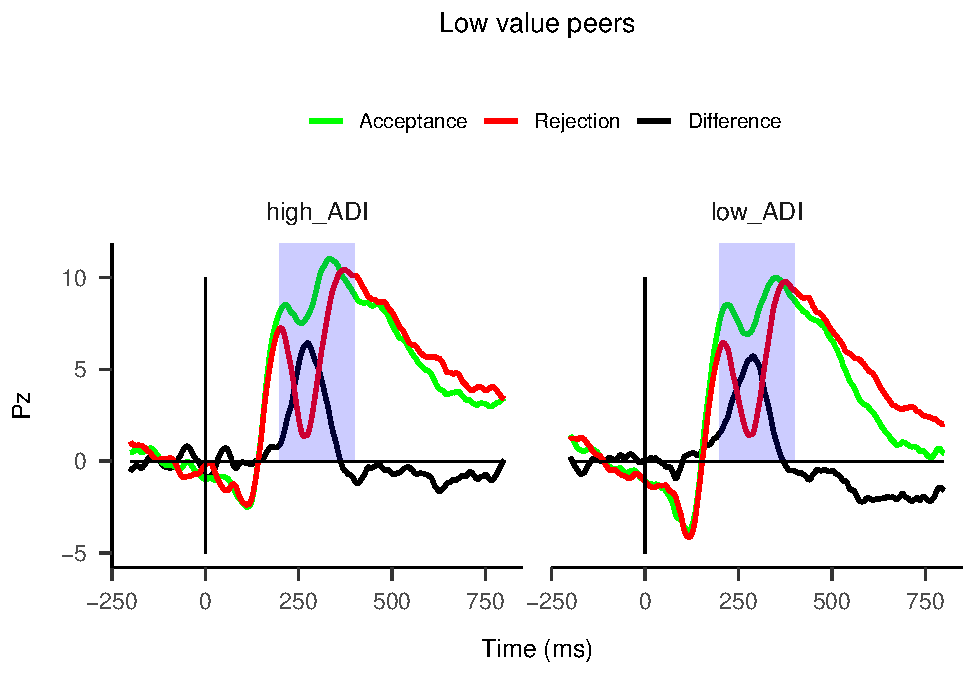
\includegraphics{do01_BUDS_files/figure-latex/unnamed-chunk-11-2.pdf}
High ADI participants show an enhanced P300 to high value rejection
relative to acceptance.

\hypertarget{plot-scalp-topographies}{%
\subsubsection{Plot scalp topographies}\label{plot-scalp-topographies}}

\begin{Shaded}
\begin{Highlighting}[]
\FunctionTok{topoplot}\NormalTok{(eeg.map\_for\_plotting\_adi\_150350, }\AttributeTok{palette=}\StringTok{"Spectral"}\NormalTok{, }\AttributeTok{chanLocs=}\NormalTok{chanlocs, }\AttributeTok{contour=}\ConstantTok{FALSE}\NormalTok{, }\AttributeTok{interp\_limit=}\StringTok{"head"}\NormalTok{, }\AttributeTok{chan\_marker=}\StringTok{"name"}\NormalTok{)}
\FunctionTok{topoplot}\NormalTok{(}\FunctionTok{filter}\NormalTok{(eeg.map\_for\_plotting\_adi\_150350, adi\_median\_split}\SpecialCharTok{==}\StringTok{"high\_ADI"}\NormalTok{), }\AttributeTok{palette=}\StringTok{"Spectral"}\NormalTok{, }\AttributeTok{chanLocs=}\NormalTok{chanlocs, }\AttributeTok{contour=}\ConstantTok{FALSE}\NormalTok{, }\AttributeTok{interp\_limit=}\StringTok{"head"}\NormalTok{, }\AttributeTok{chan\_marker=}\StringTok{"name"}\NormalTok{)}
\FunctionTok{topoplot}\NormalTok{(}\FunctionTok{filter}\NormalTok{(eeg.map\_for\_plotting\_adi\_150350, adi\_median\_split}\SpecialCharTok{==}\StringTok{"low\_ADI"}\NormalTok{), }\AttributeTok{palette=}\StringTok{"Spectral"}\NormalTok{, }\AttributeTok{chanLocs=}\NormalTok{chanlocs, }\AttributeTok{contour=}\ConstantTok{FALSE}\NormalTok{, }\AttributeTok{interp\_limit=}\StringTok{"head"}\NormalTok{, }\AttributeTok{chan\_marker=}\StringTok{"name"}\NormalTok{)}


\FunctionTok{topoplot}\NormalTok{(eeg.map\_for\_plotting\_adi\_250500, }\AttributeTok{palette=}\StringTok{"Spectral"}\NormalTok{, }\AttributeTok{chanLocs=}\NormalTok{chanlocs, }\AttributeTok{contour=}\ConstantTok{FALSE}\NormalTok{, }\AttributeTok{interp\_limit=}\StringTok{"head"}\NormalTok{, }\AttributeTok{chan\_marker=}\StringTok{"name"}\NormalTok{)}
\FunctionTok{topoplot}\NormalTok{(}\FunctionTok{filter}\NormalTok{(eeg.map\_for\_plotting\_adi\_250500, adi\_median\_split}\SpecialCharTok{==}\StringTok{"high\_ADI"}\NormalTok{), }\AttributeTok{palette=}\StringTok{"Spectral"}\NormalTok{, }\AttributeTok{chanLocs=}\NormalTok{chanlocs, }\AttributeTok{contour=}\ConstantTok{FALSE}\NormalTok{, }\AttributeTok{interp\_limit=}\StringTok{"head"}\NormalTok{, }\AttributeTok{chan\_marker=}\StringTok{"name"}\NormalTok{)}
\FunctionTok{topoplot}\NormalTok{(}\FunctionTok{filter}\NormalTok{(eeg.map\_for\_plotting\_adi\_250500, adi\_median\_split}\SpecialCharTok{==}\StringTok{"low\_ADI"}\NormalTok{), }\AttributeTok{palette=}\StringTok{"Spectral"}\NormalTok{, }\AttributeTok{chanLocs=}\NormalTok{chanlocs, }\AttributeTok{contour=}\ConstantTok{FALSE}\NormalTok{, }\AttributeTok{interp\_limit=}\StringTok{"head"}\NormalTok{, }\AttributeTok{chan\_marker=}\StringTok{"name"}\NormalTok{)}

\FunctionTok{topoplot}\NormalTok{(eeg.map\_for\_plotting\_adi\_200400, }\AttributeTok{palette=}\StringTok{"Spectral"}\NormalTok{, }\AttributeTok{chanLocs=}\NormalTok{chanlocs, }\AttributeTok{contour=}\ConstantTok{FALSE}\NormalTok{, }\AttributeTok{interp\_limit=}\StringTok{"head"}\NormalTok{, }\AttributeTok{chan\_marker=}\StringTok{"name"}\NormalTok{)}
\FunctionTok{topoplot}\NormalTok{(}\FunctionTok{filter}\NormalTok{(eeg.map\_for\_plotting\_adi\_200400, adi\_median\_split}\SpecialCharTok{==}\StringTok{"high\_ADI"}\NormalTok{), }\AttributeTok{palette=}\StringTok{"Spectral"}\NormalTok{, }\AttributeTok{chanLocs=}\NormalTok{chanlocs, }\AttributeTok{contour=}\ConstantTok{FALSE}\NormalTok{, }\AttributeTok{interp\_limit=}\StringTok{"head"}\NormalTok{, }\AttributeTok{chan\_marker=}\StringTok{"name"}\NormalTok{)}
\FunctionTok{topoplot}\NormalTok{(}\FunctionTok{filter}\NormalTok{(eeg.map\_for\_plotting\_adi\_200400, adi\_median\_split}\SpecialCharTok{==}\StringTok{"low\_ADI"}\NormalTok{), }\AttributeTok{palette=}\StringTok{"Spectral"}\NormalTok{, }\AttributeTok{chanLocs=}\NormalTok{chanlocs, }\AttributeTok{contour=}\ConstantTok{FALSE}\NormalTok{, }\AttributeTok{interp\_limit=}\StringTok{"head"}\NormalTok{, }\AttributeTok{chan\_marker=}\StringTok{"name"}\NormalTok{)}

\FunctionTok{topoplot}\NormalTok{(eeg.map\_for\_plotting\_adi\_150275, }\AttributeTok{palette=}\StringTok{"Spectral"}\NormalTok{, }\AttributeTok{chanLocs=}\NormalTok{chanlocs, }\AttributeTok{contour=}\ConstantTok{FALSE}\NormalTok{, }\AttributeTok{interp\_limit=}\StringTok{"head"}\NormalTok{, }\AttributeTok{chan\_marker=}\StringTok{"name"}\NormalTok{)}
\FunctionTok{topoplot}\NormalTok{(}\FunctionTok{filter}\NormalTok{(eeg.map\_for\_plotting\_adi\_150275, adi\_median\_split}\SpecialCharTok{==}\StringTok{"high\_ADI"}\NormalTok{), }\AttributeTok{palette=}\StringTok{"Spectral"}\NormalTok{, }\AttributeTok{chanLocs=}\NormalTok{chanlocs, }\AttributeTok{contour=}\ConstantTok{FALSE}\NormalTok{, }\AttributeTok{interp\_limit=}\StringTok{"head"}\NormalTok{, }\AttributeTok{chan\_marker=}\StringTok{"name"}\NormalTok{)}
\FunctionTok{topoplot}\NormalTok{(}\FunctionTok{filter}\NormalTok{(eeg.map\_for\_plotting\_adi\_150275, adi\_median\_split}\SpecialCharTok{==}\StringTok{"low\_ADI"}\NormalTok{), }\AttributeTok{palette=}\StringTok{"Spectral"}\NormalTok{, }\AttributeTok{chanLocs=}\NormalTok{chanlocs, }\AttributeTok{contour=}\ConstantTok{FALSE}\NormalTok{, }\AttributeTok{interp\_limit=}\StringTok{"head"}\NormalTok{, }\AttributeTok{chan\_marker=}\StringTok{"name"}\NormalTok{)}

\FunctionTok{topoplot}\NormalTok{(eeg.map\_for\_plotting\_adi\_50150, }\AttributeTok{palette=}\StringTok{"Spectral"}\NormalTok{, }\AttributeTok{chanLocs=}\NormalTok{chanlocs, }\AttributeTok{contour=}\ConstantTok{FALSE}\NormalTok{, }\AttributeTok{interp\_limit=}\StringTok{"head"}\NormalTok{, }\AttributeTok{chan\_marker=}\StringTok{"name"}\NormalTok{)}
\FunctionTok{topoplot}\NormalTok{(}\FunctionTok{filter}\NormalTok{(eeg.map\_for\_plotting\_adi\_50150, adi\_median\_split}\SpecialCharTok{==}\StringTok{"high\_ADI"}\NormalTok{), }\AttributeTok{palette=}\StringTok{"Spectral"}\NormalTok{, }\AttributeTok{chanLocs=}\NormalTok{chanlocs, }\AttributeTok{contour=}\ConstantTok{FALSE}\NormalTok{, }\AttributeTok{interp\_limit=}\StringTok{"head"}\NormalTok{, }\AttributeTok{chan\_marker=}\StringTok{"name"}\NormalTok{)}
\FunctionTok{topoplot}\NormalTok{(}\FunctionTok{filter}\NormalTok{(eeg.map\_for\_plotting\_adi\_50150, adi\_median\_split}\SpecialCharTok{==}\StringTok{"low\_ADI"}\NormalTok{), }\AttributeTok{palette=}\StringTok{"Spectral"}\NormalTok{, }\AttributeTok{chanLocs=}\NormalTok{chanlocs, }\AttributeTok{contour=}\ConstantTok{FALSE}\NormalTok{, }\AttributeTok{interp\_limit=}\StringTok{"head"}\NormalTok{, }\AttributeTok{chan\_marker=}\StringTok{"name"}\NormalTok{)}
\end{Highlighting}
\end{Shaded}

\hypertarget{strain}{%
\section{STRAIN}\label{strain}}

\begin{Shaded}
\begin{Highlighting}[]
\FunctionTok{load}\NormalTok{(}\FunctionTok{here}\NormalTok{(}\StringTok{"data/BUDS\_cleaning02\_with\_strain.RData"}\NormalTok{))}
\NormalTok{BUDS\_cleaning02\_with\_strain}\SpecialCharTok{$}\NormalTok{ID }\OtherTok{\textless{}{-}} \FunctionTok{as.integer}\NormalTok{(}\FunctionTok{as.character}\NormalTok{(BUDS\_cleaning02\_with\_strain}\SpecialCharTok{$}\NormalTok{id\_1\_i))}

\NormalTok{df\_275425\_pooled\_strain }\OtherTok{\textless{}{-}}\NormalTok{ df\_275425\_pooled }\SpecialCharTok{\%\textgreater{}\%}
  \FunctionTok{full\_join}\NormalTok{(BUDS\_cleaning02\_with\_strain, }\AttributeTok{by=}\StringTok{"ID"}\NormalTok{)}

\NormalTok{df\_275425\_cz\_strain }\OtherTok{\textless{}{-}}\NormalTok{ df\_275425\_cz }\SpecialCharTok{\%\textgreater{}\%}
  \FunctionTok{full\_join}\NormalTok{(BUDS\_cleaning02\_with\_strain, }\AttributeTok{by=}\StringTok{"ID"}\NormalTok{)}

\NormalTok{df\_150350\_cz\_strain }\OtherTok{\textless{}{-}}\NormalTok{ df\_150350\_cz }\SpecialCharTok{\%\textgreater{}\%}
  \FunctionTok{full\_join}\NormalTok{(BUDS\_cleaning02\_with\_strain, }\AttributeTok{by=}\StringTok{"ID"}\NormalTok{)}
  
\NormalTok{df\_250450\_fz\_strain }\OtherTok{\textless{}{-}}\NormalTok{ df\_250450\_fz }\SpecialCharTok{\%\textgreater{}\%}
  \FunctionTok{full\_join}\NormalTok{(BUDS\_cleaning02\_with\_strain, }\AttributeTok{by=}\StringTok{"ID"}\NormalTok{)}

\NormalTok{df\_200400\_pz\_strain }\OtherTok{\textless{}{-}}\NormalTok{ df\_200400\_pz }\SpecialCharTok{\%\textgreater{}\%}
  \FunctionTok{full\_join}\NormalTok{(BUDS\_cleaning02\_with\_strain, }\AttributeTok{by=}\StringTok{"ID"}\NormalTok{)}

\NormalTok{df\_150275\_cz\_strain }\OtherTok{\textless{}{-}}\NormalTok{ df\_150275\_cz }\SpecialCharTok{\%\textgreater{}\%}
  \FunctionTok{full\_join}\NormalTok{(BUDS\_cleaning02\_with\_strain, }\AttributeTok{by=}\StringTok{"ID"}\NormalTok{)}

\NormalTok{df\_50150\_cz\_strain }\OtherTok{\textless{}{-}}\NormalTok{ df\_50150\_cz }\SpecialCharTok{\%\textgreater{}\%}
  \FunctionTok{full\_join}\NormalTok{(BUDS\_cleaning02\_with\_strain, }\AttributeTok{by=}\StringTok{"ID"}\NormalTok{)}

\CommentTok{\# df\_4001000\_pz\_strain \textless{}{-} df\_4001000\_pz \%\textgreater{}\%}
\CommentTok{\#   full\_join(BUDS\_cleaning02\_with\_strain, by="ID")}
\CommentTok{\# }
\CommentTok{\# df\_6001500\_pz\_strain \textless{}{-} df\_6001500\_pz \%\textgreater{}\%}
\CommentTok{\#   full\_join(BUDS\_cleaning02\_with\_strain, by="ID")}

\NormalTok{df\_150350\_cz\_long\_strain }\OtherTok{\textless{}{-}}\NormalTok{ df\_150350\_cz\_long }\SpecialCharTok{\%\textgreater{}\%}
  \FunctionTok{full\_join}\NormalTok{(BUDS\_cleaning02\_with\_strain, }\AttributeTok{by=}\StringTok{"ID"}\NormalTok{, }\AttributeTok{relationship =} \StringTok{"many{-}to{-}many"}\NormalTok{)}

\NormalTok{df\_200400\_pz\_long\_strain }\OtherTok{\textless{}{-}}\NormalTok{ df\_200400\_pz\_long }\SpecialCharTok{\%\textgreater{}\%}
  \FunctionTok{full\_join}\NormalTok{(BUDS\_cleaning02\_with\_strain, }\AttributeTok{by=}\StringTok{"ID"}\NormalTok{, }\AttributeTok{relationship =} \StringTok{"many{-}to{-}many"}\NormalTok{)}

\NormalTok{df\_250450\_fz\_long\_strain }\OtherTok{\textless{}{-}}\NormalTok{ df\_250450\_fz\_long }\SpecialCharTok{\%\textgreater{}\%}
  \FunctionTok{full\_join}\NormalTok{(BUDS\_cleaning02\_with\_strain, }\AttributeTok{by=}\StringTok{"ID"}\NormalTok{, }\AttributeTok{relationship =} \StringTok{"many{-}to{-}many"}\NormalTok{)}

\NormalTok{df\_275425\_pooled\_long\_strain }\OtherTok{\textless{}{-}}\NormalTok{ df\_275425\_pooled\_long }\SpecialCharTok{\%\textgreater{}\%}
  \FunctionTok{full\_join}\NormalTok{(BUDS\_cleaning02\_with\_strain, }\AttributeTok{by=}\StringTok{"ID"}\NormalTok{, }\AttributeTok{relationship =} \StringTok{"many{-}to{-}many"}\NormalTok{)}

\NormalTok{df\_275425\_cz\_long\_strain }\OtherTok{\textless{}{-}}\NormalTok{ df\_275425\_cz\_long }\SpecialCharTok{\%\textgreater{}\%}
  \FunctionTok{full\_join}\NormalTok{(BUDS\_cleaning02\_with\_strain, }\AttributeTok{by=}\StringTok{"ID"}\NormalTok{, }\AttributeTok{relationship =} \StringTok{"many{-}to{-}many"}\NormalTok{)}

\NormalTok{df\_150275\_cz\_long\_strain }\OtherTok{\textless{}{-}}\NormalTok{ df\_150275\_cz\_long }\SpecialCharTok{\%\textgreater{}\%}
  \FunctionTok{full\_join}\NormalTok{(BUDS\_cleaning02\_with\_strain, }\AttributeTok{by=}\StringTok{"ID"}\NormalTok{, }\AttributeTok{relationship =} \StringTok{"many{-}to{-}many"}\NormalTok{)}

\NormalTok{df\_50150\_cz\_long\_strain }\OtherTok{\textless{}{-}}\NormalTok{ df\_50150\_cz\_long }\SpecialCharTok{\%\textgreater{}\%}
  \FunctionTok{full\_join}\NormalTok{(BUDS\_cleaning02\_with\_strain, }\AttributeTok{by=}\StringTok{"ID"}\NormalTok{, }\AttributeTok{relationship =} \StringTok{"many{-}to{-}many"}\NormalTok{)}
\end{Highlighting}
\end{Shaded}

\hypertarget{stressors-and-adi}{%
\subsection{Stressors and ADI}\label{stressors-and-adi}}

\begin{Shaded}
\begin{Highlighting}[]
\NormalTok{STRAIN\_scales }\OtherTok{\textless{}{-}} \FunctionTok{c}\NormalTok{(}\StringTok{"StressCT"}\NormalTok{, }\StringTok{"StressTH"}\NormalTok{, }\StringTok{"EvntCT"}\NormalTok{, }\StringTok{"DiffCT"}\NormalTok{, }\StringTok{"EvntTH"}\NormalTok{, }\StringTok{"DiffTH"}\NormalTok{, }\StringTok{"RecTotCT"}\NormalTok{, }\StringTok{"RecTotTH"}\NormalTok{, }\StringTok{"DHEvntCT"}\NormalTok{, }\StringTok{"DHDiffCT"}\NormalTok{, }\StringTok{"DHAllCT"}\NormalTok{, }\StringTok{"DHEvntTH"}\NormalTok{, }\StringTok{"DHDiffTH"}\NormalTok{, }\StringTok{"DHAllTH"}\NormalTok{, }\StringTok{"DEEvntCT"}\NormalTok{, }\StringTok{"DEDiffCT"}\NormalTok{, }\StringTok{"DEAllCT"}\NormalTok{, }\StringTok{"DEEvntTH"}\NormalTok{, }\StringTok{"DEDiffTH"}\NormalTok{, }\StringTok{"DEAllTH"}\NormalTok{, }\StringTok{"DWEvntCT"}\NormalTok{, }\StringTok{"DWDiffCT"}\NormalTok{, }\StringTok{"DWAllCT"}\NormalTok{, }\StringTok{"DWEvntTH"}\NormalTok{, }\StringTok{"DWDiffTH"}\NormalTok{, }\StringTok{"DWAllTH"}\NormalTok{, }\StringTok{"DTEvntCT"}\NormalTok{, }\StringTok{"DTDiffCT"}\NormalTok{, }\StringTok{"DTAllCT"}\NormalTok{, }\StringTok{"DTEvntTH"}\NormalTok{, }\StringTok{"DTDiffTH"}\NormalTok{, }\StringTok{"DTAllTH"}\NormalTok{, }\StringTok{"DMEvntCT"}\NormalTok{, }\StringTok{"DMDiffCT"}\NormalTok{, }\StringTok{"DMAllCT"}\NormalTok{, }\StringTok{"DMEvntTH"}\NormalTok{, }\StringTok{"DMDiffTH"}\NormalTok{, }\StringTok{"DMAllTH"}\NormalTok{, }\StringTok{"DREvntCT"}\NormalTok{, }\StringTok{"DRAllCT"}\NormalTok{, }\StringTok{"DREvntTH"}\NormalTok{, }\StringTok{"DRAllTH"}\NormalTok{, }\StringTok{"DFEvntCT"}\NormalTok{, }\StringTok{"DFDiffCT"}\NormalTok{, }\StringTok{"DFAllCT"}\NormalTok{, }\StringTok{"DFEvntTH"}\NormalTok{, }\StringTok{"DFDiffTH"}\NormalTok{, }\StringTok{"DFAllTH"}\NormalTok{, }\StringTok{"DLEvntCT"}\NormalTok{, }\StringTok{"DLDiffCT"}\NormalTok{, }\StringTok{"DLAllCT"}\NormalTok{, }\StringTok{"DLEvntTH"}\NormalTok{, }\StringTok{"DLDiffTH"}\NormalTok{, }\StringTok{"DLAllTH"}\NormalTok{, }\StringTok{"DOEvntCT"}\NormalTok{, }\StringTok{"DODiffCT"}\NormalTok{, }\StringTok{"DOAllCT"}\NormalTok{, }\StringTok{"DOEvntTH"}\NormalTok{, }\StringTok{"DODiffTH"}\NormalTok{, }\StringTok{"DOAllTH"}\NormalTok{, }\StringTok{"DDEvntCT"}\NormalTok{, }\StringTok{"DDDiffCT"}\NormalTok{, }\StringTok{"DDAllCT"}\NormalTok{, }\StringTok{"DDEvntTH"}\NormalTok{, }\StringTok{"DDDiffTH"}\NormalTok{, }\StringTok{"DDAllTH"}\NormalTok{, }\StringTok{"DXEvntCT"}\NormalTok{, }\StringTok{"DXAllCT"}\NormalTok{, }\StringTok{"DXEvntTH"}\NormalTok{, }\StringTok{"DXAllTH"}\NormalTok{, }\StringTok{"DGEvntCT"}\NormalTok{, }\StringTok{"DGDiffCT"}\NormalTok{, }\StringTok{"DGAllCT"}\NormalTok{, }\StringTok{"DGEvntTH"}\NormalTok{, }\StringTok{"DGDiffTH"}\NormalTok{, }\StringTok{"DGAllTH"}\NormalTok{, }\StringTok{"CIEvntCT"}\NormalTok{, }\StringTok{"CIDiffCT"}\NormalTok{, }\StringTok{"CIAllCT"}\NormalTok{, }\StringTok{"CIEvntTH"}\NormalTok{, }\StringTok{"CIDiffTH"}\NormalTok{, }\StringTok{"CIAllTH"}\NormalTok{, }\StringTok{"CDEvntCT"}\NormalTok{, }\StringTok{"CDDiffCT"}\NormalTok{, }\StringTok{"CDAllCT"}\NormalTok{, }\StringTok{"CDEvntTH"}\NormalTok{, }\StringTok{"CDDiffTH"}\NormalTok{, }\StringTok{"CDAllTH"}\NormalTok{, }\StringTok{"CHEvntCT"}\NormalTok{, }\StringTok{"CHDiffCT"}\NormalTok{, }\StringTok{"CHAllCT"}\NormalTok{, }\StringTok{"CHEvntTH"}\NormalTok{, }\StringTok{"CHDiffTH"}\NormalTok{, }\StringTok{"CHAllTH"}\NormalTok{, }\StringTok{"CEEvntCT"}\NormalTok{, }\StringTok{"CEDiffCT"}\NormalTok{, }\StringTok{"CEAllCT"}\NormalTok{, }\StringTok{"CEEvntTH"}\NormalTok{, }\StringTok{"CEDiffTH"}\NormalTok{, }\StringTok{"CEAllTH"}\NormalTok{, }\StringTok{"CREvntCT"}\NormalTok{, }\StringTok{"CRDiffCT"}\NormalTok{, }\StringTok{"CRAllCT"}\NormalTok{, }\StringTok{"CREvntTH"}\NormalTok{, }\StringTok{"CRDiffTH"}\NormalTok{, }\StringTok{"CRAllTH"}\NormalTok{)}

\ControlFlowTok{for}\NormalTok{ (p }\ControlFlowTok{in}\NormalTok{ STRAIN\_scales) \{}
  \ControlFlowTok{for}\NormalTok{ (data }\ControlFlowTok{in} \FunctionTok{c}\NormalTok{(}\StringTok{"df\_150350\_cz\_strain"}\NormalTok{)) \{}
  \ControlFlowTok{for}\NormalTok{ (comp }\ControlFlowTok{in} \FunctionTok{c}\NormalTok{(}\StringTok{"ADI\_NATRANK\_log\_z"}\NormalTok{)) \{}
      \FunctionTok{eval}\NormalTok{(}\FunctionTok{parse}\NormalTok{(}\AttributeTok{text=}\FunctionTok{paste0}\NormalTok{(}\StringTok{\textquotesingle{}print(summary(lm(\textquotesingle{}}\NormalTok{,comp,}\StringTok{\textquotesingle{} \textasciitilde{} \textquotesingle{}}\NormalTok{,p,}\StringTok{\textquotesingle{}, \textquotesingle{}}\NormalTok{,data,}\StringTok{\textquotesingle{}))$call)}
\StringTok{                             print(summary(lm(\textquotesingle{}}\NormalTok{,comp,}\StringTok{\textquotesingle{} \textasciitilde{} \textquotesingle{}}\NormalTok{,p,}\StringTok{\textquotesingle{}, \textquotesingle{}}\NormalTok{,data,}\StringTok{\textquotesingle{}))$coef[2,4])\textquotesingle{}}\NormalTok{)))}
\NormalTok{  \}\}\}}

\CommentTok{\# Domain: Reproduction}
\FunctionTok{lm}\NormalTok{(}\AttributeTok{formula =}\NormalTok{ ADI\_NATRANK\_log\_z }\SpecialCharTok{\textasciitilde{}}\NormalTok{ DREvntTH, }\AttributeTok{data =}\NormalTok{ df\_150350\_cz\_strain)}
\FunctionTok{lm}\NormalTok{(}\AttributeTok{formula =}\NormalTok{ ADI\_NATRANK\_log\_z }\SpecialCharTok{\textasciitilde{}}\NormalTok{ DRAllTH, }\AttributeTok{data =}\NormalTok{ df\_150350\_cz\_strain)}

\CommentTok{\# Characteristic: Entrapment}
\FunctionTok{lm}\NormalTok{(}\AttributeTok{formula =}\NormalTok{ ADI\_NATRANK\_log\_z }\SpecialCharTok{\textasciitilde{}}\NormalTok{ CEEvntCT, }\AttributeTok{data =}\NormalTok{ df\_150350\_cz\_strain)}

\CommentTok{\# Characteristic: Role Change/Reversal}
\FunctionTok{lm}\NormalTok{(}\AttributeTok{formula =}\NormalTok{ ADI\_NATRANK\_log\_z }\SpecialCharTok{\textasciitilde{}}\NormalTok{ CRDiffCT, }\AttributeTok{data =}\NormalTok{ df\_150350\_cz\_strain)}
\FunctionTok{lm}\NormalTok{(}\AttributeTok{formula =}\NormalTok{ ADI\_NATRANK\_log\_z }\SpecialCharTok{\textasciitilde{}}\NormalTok{ CRAllCT, }\AttributeTok{data =}\NormalTok{ df\_150350\_cz\_strain)}
\FunctionTok{lm}\NormalTok{(}\AttributeTok{formula =}\NormalTok{ ADI\_NATRANK\_log\_z }\SpecialCharTok{\textasciitilde{}}\NormalTok{ CRDiffTH, }\AttributeTok{data =}\NormalTok{ df\_150350\_cz\_strain)}
\FunctionTok{lm}\NormalTok{(}\AttributeTok{formula =}\NormalTok{ ADI\_NATRANK\_log\_z }\SpecialCharTok{\textasciitilde{}}\NormalTok{ CRAllTH, }\AttributeTok{data =}\NormalTok{ df\_150350\_cz\_strain)}

\CommentTok{\# Housing related stressors}
\FunctionTok{lm}\NormalTok{(}\AttributeTok{formula =}\NormalTok{ ADI\_NATRANK\_log\_z }\SpecialCharTok{\textasciitilde{}}\NormalTok{ DHEvntCT, }\AttributeTok{data =}\NormalTok{ df\_150350\_cz\_strain)}
\FunctionTok{lm}\NormalTok{(}\AttributeTok{formula =}\NormalTok{ ADI\_NATRANK\_log\_z }\SpecialCharTok{\textasciitilde{}}\NormalTok{ DHAllCT, }\AttributeTok{data =}\NormalTok{ df\_150350\_cz\_strain)}
\FunctionTok{lm}\NormalTok{(}\AttributeTok{formula =}\NormalTok{ ADI\_NATRANK\_log\_z }\SpecialCharTok{\textasciitilde{}}\NormalTok{ DHEvntTH, }\AttributeTok{data =}\NormalTok{ df\_150350\_cz\_strain)}

\CommentTok{\# Domain: Treatment/Health {-} Count of Chronic Difficulties}
\FunctionTok{lm}\NormalTok{(}\AttributeTok{formula =}\NormalTok{ ADI\_NATRANK\_log\_z }\SpecialCharTok{\textasciitilde{}}\NormalTok{ DTDiffCT, }\AttributeTok{data =}\NormalTok{ df\_150350\_cz\_strain)}

\FunctionTok{summary}\NormalTok{(}\FunctionTok{lm}\NormalTok{(AR\_AA }\SpecialCharTok{\textasciitilde{}}\NormalTok{ ADI\_NATRANK\_log\_z }\SpecialCharTok{+}\NormalTok{ StressCT }\SpecialCharTok{+}\NormalTok{ StressTH }\SpecialCharTok{+}\NormalTok{ Age }\SpecialCharTok{+}\NormalTok{ Sex, df\_150350\_cz\_strain))}
\FunctionTok{summary}\NormalTok{(}\FunctionTok{lm}\NormalTok{(AR\_AA }\SpecialCharTok{\textasciitilde{}}\NormalTok{ ADI\_NATRANK\_log\_z }\SpecialCharTok{+}\NormalTok{ StressCT }\SpecialCharTok{+}\NormalTok{ StressTH }\SpecialCharTok{+}\NormalTok{ Age }\SpecialCharTok{+}\NormalTok{ Sex, df\_250450\_fz\_strain))}
\FunctionTok{summary}\NormalTok{(}\FunctionTok{lm}\NormalTok{(AR\_AA }\SpecialCharTok{\textasciitilde{}}\NormalTok{ ADI\_NATRANK\_log\_z }\SpecialCharTok{+}\NormalTok{ StressCT }\SpecialCharTok{+}\NormalTok{ StressTH }\SpecialCharTok{+}\NormalTok{ Age }\SpecialCharTok{+}\NormalTok{ Sex, df\_200400\_pz\_strain))}

\ControlFlowTok{for}\NormalTok{ (p }\ControlFlowTok{in}\NormalTok{ STRAIN\_scales) \{}
  \ControlFlowTok{for}\NormalTok{ (data }\ControlFlowTok{in} \FunctionTok{c}\NormalTok{(}\StringTok{"df\_150350\_cz\_strain"}\NormalTok{,}\StringTok{"df\_250450\_fz\_strain"}\NormalTok{,}\StringTok{"df\_200400\_pz\_strain"}\NormalTok{)) \{}
  \ControlFlowTok{for}\NormalTok{ (comp }\ControlFlowTok{in} \FunctionTok{c}\NormalTok{(}\StringTok{"RR\_RA"}\NormalTok{)) \{}
      \FunctionTok{eval}\NormalTok{(}\FunctionTok{parse}\NormalTok{(}\AttributeTok{text=}\FunctionTok{paste0}\NormalTok{(}\StringTok{\textquotesingle{}print(summary(lm(\textquotesingle{}}\NormalTok{,comp,}\StringTok{\textquotesingle{} \textasciitilde{} \textquotesingle{}}\NormalTok{,p,}\StringTok{\textquotesingle{}, \textquotesingle{}}\NormalTok{,data,}\StringTok{\textquotesingle{}))$call)}
\StringTok{                             print(summary(lm(\textquotesingle{}}\NormalTok{,comp,}\StringTok{\textquotesingle{} \textasciitilde{} \textquotesingle{}}\NormalTok{,p,}\StringTok{\textquotesingle{}, \textquotesingle{}}\NormalTok{,data,}\StringTok{\textquotesingle{}))$coef[2,4])\textquotesingle{}}\NormalTok{)))}
\NormalTok{  \}\}\}}

\FunctionTok{lm}\NormalTok{(}\AttributeTok{formula =}\NormalTok{ AR\_AA }\SpecialCharTok{\textasciitilde{}}\NormalTok{ DMDiffCT, }\AttributeTok{data =}\NormalTok{ df\_250450\_fz\_strain)}
\FunctionTok{lm}\NormalTok{(}\AttributeTok{formula =}\NormalTok{ AR\_AA }\SpecialCharTok{\textasciitilde{}}\NormalTok{ DMDiffTH, }\AttributeTok{data =}\NormalTok{ df\_250450\_fz\_strain)}
\FunctionTok{lm}\NormalTok{(}\AttributeTok{formula =}\NormalTok{ AR\_AA }\SpecialCharTok{\textasciitilde{}}\NormalTok{ DGEvntCT, }\AttributeTok{data =}\NormalTok{ df\_200400\_pz\_strain)}
\end{Highlighting}
\end{Shaded}

\hypertarget{significant-regression-results}{%
\subsection{Significant regression
results}\label{significant-regression-results}}

\begin{Shaded}
\begin{Highlighting}[]
\CommentTok{\# Response to rejection relative to acceptance from high value peers is consistently related to ADI across components}
\FunctionTok{ggplot}\NormalTok{(df\_150350\_cz, }\FunctionTok{aes}\NormalTok{(}\AttributeTok{x=}\NormalTok{AR\_AA, }\AttributeTok{y=}\NormalTok{ADI\_NATRANK\_log)) }\SpecialCharTok{+}
  \FunctionTok{geom\_point}\NormalTok{() }\SpecialCharTok{+}
  \FunctionTok{stat\_smooth}\NormalTok{(}\AttributeTok{method=}\StringTok{"lm"}\NormalTok{) }\SpecialCharTok{+}
  \FunctionTok{geom\_text}\NormalTok{(}\AttributeTok{x=}\SpecialCharTok{{-}}\DecValTok{2}\NormalTok{, }\AttributeTok{y=}\NormalTok{.}\DecValTok{5}\NormalTok{, }\AttributeTok{color=}\StringTok{"blue"}\NormalTok{, }\AttributeTok{size=}\DecValTok{5}\NormalTok{, }\AttributeTok{label=}\FunctionTok{paste0}\NormalTok{(}\StringTok{"beta="}\NormalTok{,}
       \FunctionTok{round}\NormalTok{(}\FunctionTok{tidy}\NormalTok{(}\FunctionTok{lm}\NormalTok{(}\AttributeTok{formula =}\NormalTok{ ADI\_NATRANK\_log\_z }\SpecialCharTok{\textasciitilde{}}\NormalTok{ AR\_AA, }\AttributeTok{data =}\NormalTok{ df\_150350\_cz))[}\DecValTok{2}\NormalTok{,}\FunctionTok{c}\NormalTok{(}\DecValTok{2}\NormalTok{)],}\DecValTok{3}\NormalTok{),}
       \StringTok{", p="}\NormalTok{, }
       \FunctionTok{round}\NormalTok{(}\FunctionTok{tidy}\NormalTok{(}\FunctionTok{lm}\NormalTok{(}\AttributeTok{formula =}\NormalTok{ ADI\_NATRANK\_log\_z }\SpecialCharTok{\textasciitilde{}}\NormalTok{ AR\_AA, }\AttributeTok{data =}\NormalTok{ df\_150350\_cz))[}\DecValTok{2}\NormalTok{,}\FunctionTok{c}\NormalTok{(}\DecValTok{5}\NormalTok{)],}\DecValTok{3}\NormalTok{))) }\SpecialCharTok{+}
  \FunctionTok{labs}\NormalTok{(}\AttributeTok{x=}\StringTok{"High value rejection }\SpecialCharTok{\textbackslash{}n}\StringTok{(relative to high value acceptance)"}\NormalTok{,}
       \AttributeTok{y=}\StringTok{"Area Deprivation"}\NormalTok{) }\SpecialCharTok{+}
  \FunctionTok{theme}\NormalTok{(}\AttributeTok{text=}\FunctionTok{element\_text}\NormalTok{(}\AttributeTok{size=}\DecValTok{15}\NormalTok{))}
\end{Highlighting}
\end{Shaded}

\begin{verbatim}
## Warning: Removed 68 rows containing non-finite values (`stat_smooth()`).
\end{verbatim}

\begin{verbatim}
## Warning: Removed 68 rows containing missing values (`geom_point()`).
\end{verbatim}

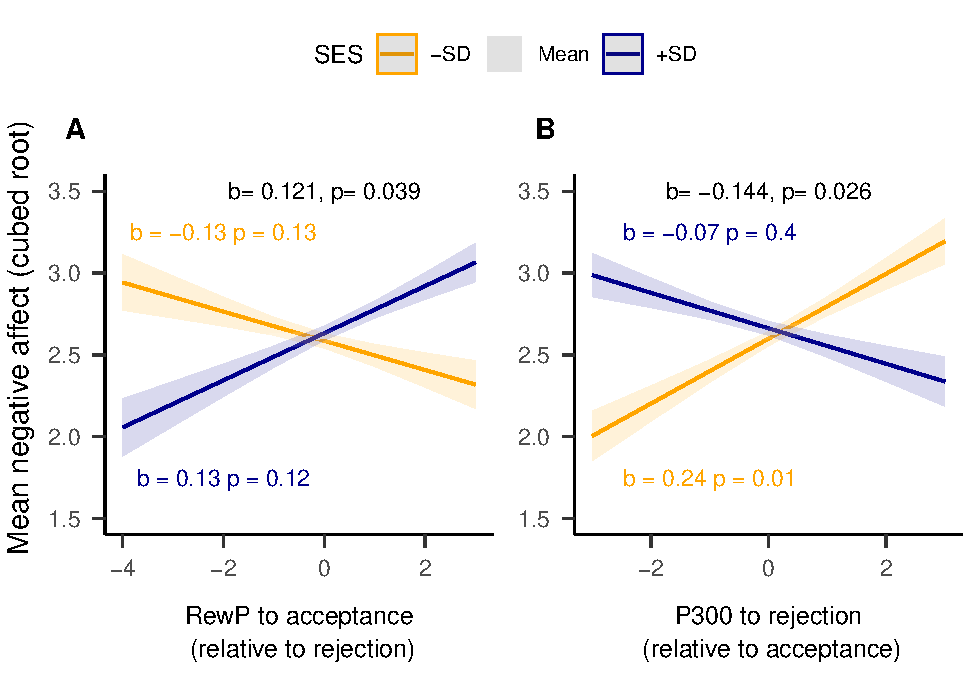
\includegraphics{do01_BUDS_files/figure-latex/unnamed-chunk-15-1.pdf}

\begin{Shaded}
\begin{Highlighting}[]
\FunctionTok{ggplot}\NormalTok{(df\_250450\_fz, }\FunctionTok{aes}\NormalTok{(}\AttributeTok{x=}\NormalTok{AR\_AA, }\AttributeTok{y=}\NormalTok{ADI\_NATRANK\_log)) }\SpecialCharTok{+}
  \FunctionTok{geom\_point}\NormalTok{() }\SpecialCharTok{+}
  \FunctionTok{stat\_smooth}\NormalTok{(}\AttributeTok{method=}\StringTok{"lm"}\NormalTok{) }\SpecialCharTok{+}
  \FunctionTok{geom\_text}\NormalTok{(}\AttributeTok{x=}\SpecialCharTok{{-}}\DecValTok{1}\NormalTok{, }\AttributeTok{y=}\NormalTok{.}\DecValTok{5}\NormalTok{, }\AttributeTok{color=}\StringTok{"blue"}\NormalTok{, }\AttributeTok{size=}\DecValTok{5}\NormalTok{, }\AttributeTok{label=}\FunctionTok{paste0}\NormalTok{(}\StringTok{"beta="}\NormalTok{,}
       \FunctionTok{round}\NormalTok{(}\FunctionTok{tidy}\NormalTok{(}\FunctionTok{lm}\NormalTok{(}\AttributeTok{formula =}\NormalTok{ ADI\_NATRANK\_log\_z }\SpecialCharTok{\textasciitilde{}}\NormalTok{ AR\_AA, }\AttributeTok{data =}\NormalTok{ df\_250450\_fz))[}\DecValTok{2}\NormalTok{,}\FunctionTok{c}\NormalTok{(}\DecValTok{2}\NormalTok{)],}\DecValTok{3}\NormalTok{),}
       \StringTok{", p="}\NormalTok{, }
       \FunctionTok{round}\NormalTok{(}\FunctionTok{tidy}\NormalTok{(}\FunctionTok{lm}\NormalTok{(}\AttributeTok{formula =}\NormalTok{ ADI\_NATRANK\_log\_z }\SpecialCharTok{\textasciitilde{}}\NormalTok{ AR\_AA, }\AttributeTok{data =}\NormalTok{ df\_250450\_fz))[}\DecValTok{2}\NormalTok{,}\FunctionTok{c}\NormalTok{(}\DecValTok{5}\NormalTok{)],}\DecValTok{3}\NormalTok{))) }\SpecialCharTok{+}
    \FunctionTok{labs}\NormalTok{(}\AttributeTok{x=}\StringTok{"High value rejection }\SpecialCharTok{\textbackslash{}n}\StringTok{(relative to high value acceptance)"}\NormalTok{,}
       \AttributeTok{y=}\StringTok{"Area Deprivation"}\NormalTok{) }\SpecialCharTok{+}
  \FunctionTok{theme}\NormalTok{(}\AttributeTok{text=}\FunctionTok{element\_text}\NormalTok{(}\AttributeTok{size=}\DecValTok{15}\NormalTok{))}
\end{Highlighting}
\end{Shaded}

\begin{verbatim}
## Warning: Removed 68 rows containing non-finite values (`stat_smooth()`).
## Removed 68 rows containing missing values (`geom_point()`).
\end{verbatim}

\includegraphics{do01_BUDS_files/figure-latex/unnamed-chunk-15-2.pdf}

\begin{Shaded}
\begin{Highlighting}[]
\FunctionTok{ggplot}\NormalTok{(df\_200400\_pz, }\FunctionTok{aes}\NormalTok{(}\AttributeTok{x=}\NormalTok{AR\_AA, }\AttributeTok{y=}\NormalTok{ADI\_NATRANK\_log)) }\SpecialCharTok{+}
  \FunctionTok{geom\_point}\NormalTok{() }\SpecialCharTok{+}
  \FunctionTok{stat\_smooth}\NormalTok{(}\AttributeTok{method=}\StringTok{"lm"}\NormalTok{) }\SpecialCharTok{+}
  \FunctionTok{geom\_text}\NormalTok{(}\AttributeTok{x=}\SpecialCharTok{{-}}\DecValTok{1}\NormalTok{, }\AttributeTok{y=}\NormalTok{.}\DecValTok{5}\NormalTok{, }\AttributeTok{color=}\StringTok{"blue"}\NormalTok{, }\AttributeTok{size=}\DecValTok{5}\NormalTok{, }\AttributeTok{label=}\FunctionTok{paste0}\NormalTok{(}\StringTok{"beta="}\NormalTok{,}
       \FunctionTok{round}\NormalTok{(}\FunctionTok{tidy}\NormalTok{(}\FunctionTok{lm}\NormalTok{(}\AttributeTok{formula =}\NormalTok{ ADI\_NATRANK\_log\_z }\SpecialCharTok{\textasciitilde{}}\NormalTok{ AR\_AA, }\AttributeTok{data =}\NormalTok{ df\_200400\_pz))[}\DecValTok{2}\NormalTok{,}\FunctionTok{c}\NormalTok{(}\DecValTok{2}\NormalTok{)],}\DecValTok{3}\NormalTok{),}
       \StringTok{", p="}\NormalTok{, }
       \FunctionTok{round}\NormalTok{(}\FunctionTok{tidy}\NormalTok{(}\FunctionTok{lm}\NormalTok{(}\AttributeTok{formula =}\NormalTok{ ADI\_NATRANK\_log\_z }\SpecialCharTok{\textasciitilde{}}\NormalTok{ AR\_AA, }\AttributeTok{data =}\NormalTok{ df\_200400\_pz))[}\DecValTok{2}\NormalTok{,}\FunctionTok{c}\NormalTok{(}\DecValTok{5}\NormalTok{)],}\DecValTok{3}\NormalTok{))) }\SpecialCharTok{+}
    \FunctionTok{labs}\NormalTok{(}\AttributeTok{x=}\StringTok{"High value rejection }\SpecialCharTok{\textbackslash{}n}\StringTok{(relative to high value acceptance)"}\NormalTok{,}
       \AttributeTok{y=}\StringTok{"Area Deprivation"}\NormalTok{) }\SpecialCharTok{+}
  \FunctionTok{theme}\NormalTok{(}\AttributeTok{text=}\FunctionTok{element\_text}\NormalTok{(}\AttributeTok{size=}\DecValTok{15}\NormalTok{))}
\end{Highlighting}
\end{Shaded}

\begin{verbatim}
## Warning: Removed 68 rows containing non-finite values (`stat_smooth()`).
## Removed 68 rows containing missing values (`geom_point()`).
\end{verbatim}

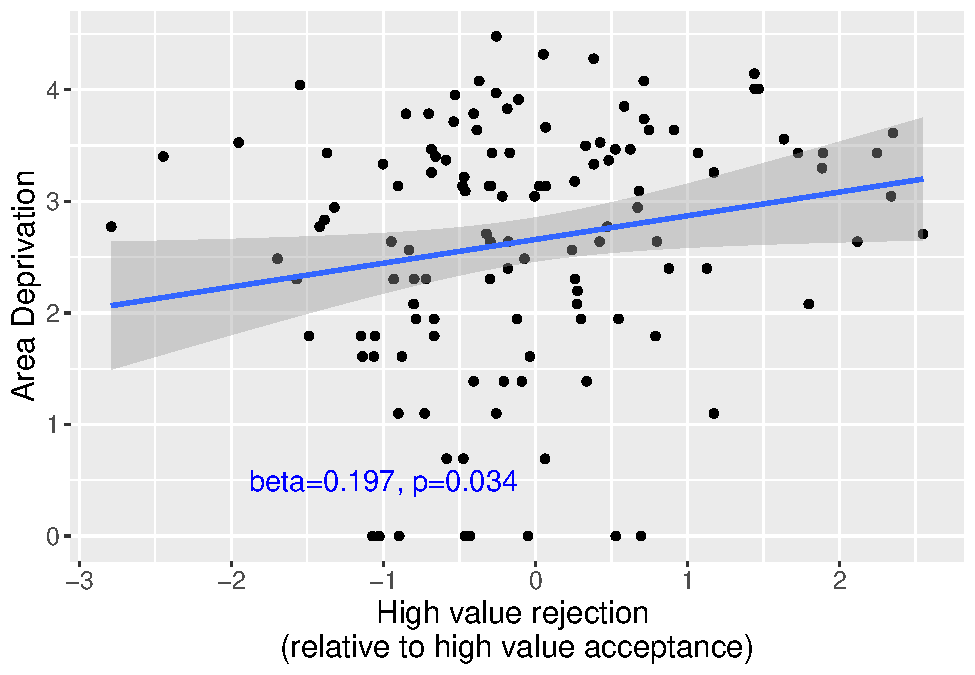
\includegraphics{do01_BUDS_files/figure-latex/unnamed-chunk-15-3.pdf}

\hypertarget{interactions}{%
\section{Interactions}\label{interactions}}

\hypertarget{adi-1}{%
\subsection{ADI}\label{adi-1}}

\begin{Shaded}
\begin{Highlighting}[]
\NormalTok{lmer\_adi\_interaction\_table }\OtherTok{\textless{}{-}} \ControlFlowTok{function}\NormalTok{(data) \{}
\NormalTok{  new\_model }\OtherTok{\textless{}{-}} \FunctionTok{data.frame}\NormalTok{(}\AttributeTok{model =} \FunctionTok{c}\NormalTok{(}\StringTok{"Both"}\NormalTok{,}\StringTok{"Like"}\NormalTok{,}\StringTok{"Dislike"}\NormalTok{),}
                            \AttributeTok{beta =} \ConstantTok{NA}\NormalTok{, }
                            \AttributeTok{p =} \ConstantTok{NA}\NormalTok{)}
\NormalTok{new\_model}\SpecialCharTok{$}\NormalTok{beta }\OtherTok{\textless{}{-}} \FunctionTok{c}\NormalTok{(broom.mixed}\SpecialCharTok{::}\FunctionTok{tidy}\NormalTok{(}\FunctionTok{lmer}\NormalTok{(}\AttributeTok{formula =}\NormalTok{ ERP }\SpecialCharTok{\textasciitilde{}}\NormalTok{ Feedback}\SpecialCharTok{*}\NormalTok{Voting}\SpecialCharTok{*}\NormalTok{ADI\_NATRANK\_log\_z }\SpecialCharTok{+}\NormalTok{ (}\DecValTok{1} \SpecialCharTok{|}\NormalTok{ ID), }\AttributeTok{data =}\NormalTok{ data))[}\DecValTok{8}\NormalTok{,}\DecValTok{4}\NormalTok{], broom.mixed}\SpecialCharTok{::}\FunctionTok{tidy}\NormalTok{(}\FunctionTok{lmer}\NormalTok{(}\AttributeTok{formula =}\NormalTok{ ERP }\SpecialCharTok{\textasciitilde{}}\NormalTok{ Feedback}\SpecialCharTok{*}\NormalTok{ADI\_NATRANK\_log\_z }\SpecialCharTok{+}\NormalTok{ (}\DecValTok{1} \SpecialCharTok{|}\NormalTok{ ID), }\AttributeTok{data =} \FunctionTok{filter}\NormalTok{(data, Voting}\SpecialCharTok{==}\StringTok{"Like"}\NormalTok{)))[}\DecValTok{4}\NormalTok{,}\DecValTok{4}\NormalTok{],}
\NormalTok{                        broom.mixed}\SpecialCharTok{::}\FunctionTok{tidy}\NormalTok{(}\FunctionTok{lmer}\NormalTok{(}\AttributeTok{formula =}\NormalTok{ ERP }\SpecialCharTok{\textasciitilde{}}\NormalTok{ Feedback}\SpecialCharTok{*}\NormalTok{ADI\_NATRANK\_log\_z }\SpecialCharTok{+}\NormalTok{ (}\DecValTok{1} \SpecialCharTok{|}\NormalTok{ ID), }\AttributeTok{data =} \FunctionTok{filter}\NormalTok{(data, Voting}\SpecialCharTok{==}\StringTok{"Dislike"}\NormalTok{)))[}\DecValTok{4}\NormalTok{,}\DecValTok{4}\NormalTok{])}

\NormalTok{new\_model}\SpecialCharTok{$}\NormalTok{p }\OtherTok{\textless{}{-}} \FunctionTok{c}\NormalTok{(broom.mixed}\SpecialCharTok{::}\FunctionTok{tidy}\NormalTok{(}\FunctionTok{lmer}\NormalTok{(}\AttributeTok{formula =}\NormalTok{ ERP }\SpecialCharTok{\textasciitilde{}}\NormalTok{ Feedback}\SpecialCharTok{*}\NormalTok{Voting}\SpecialCharTok{*}\NormalTok{ADI\_NATRANK\_log\_z }\SpecialCharTok{+}\NormalTok{ (}\DecValTok{1} \SpecialCharTok{|}\NormalTok{ ID), }\AttributeTok{data =}\NormalTok{ data))[}\DecValTok{8}\NormalTok{,}\DecValTok{8}\NormalTok{], broom.mixed}\SpecialCharTok{::}\FunctionTok{tidy}\NormalTok{(}\FunctionTok{lmer}\NormalTok{(}\AttributeTok{formula =}\NormalTok{ ERP }\SpecialCharTok{\textasciitilde{}}\NormalTok{ Feedback}\SpecialCharTok{*}\NormalTok{ADI\_NATRANK\_log\_z }\SpecialCharTok{+}\NormalTok{ (}\DecValTok{1} \SpecialCharTok{|}\NormalTok{ ID), }\AttributeTok{data =} \FunctionTok{filter}\NormalTok{(data, Voting}\SpecialCharTok{==}\StringTok{"Like"}\NormalTok{)))[}\DecValTok{4}\NormalTok{,}\DecValTok{8}\NormalTok{],}
\NormalTok{                        broom.mixed}\SpecialCharTok{::}\FunctionTok{tidy}\NormalTok{(}\FunctionTok{lmer}\NormalTok{(}\AttributeTok{formula =}\NormalTok{ ERP }\SpecialCharTok{\textasciitilde{}}\NormalTok{ Feedback}\SpecialCharTok{*}\NormalTok{ADI\_NATRANK\_log\_z }\SpecialCharTok{+}\NormalTok{ (}\DecValTok{1} \SpecialCharTok{|}\NormalTok{ ID), }\AttributeTok{data =} \FunctionTok{filter}\NormalTok{(data, Voting}\SpecialCharTok{==}\StringTok{"Dislike"}\NormalTok{)))[}\DecValTok{4}\NormalTok{,}\DecValTok{8}\NormalTok{])}
\NormalTok{new\_model}
\NormalTok{\}}
\end{Highlighting}
\end{Shaded}

\hypertarget{cz}{%
\subsubsection{150-350 Cz}\label{cz}}

\begin{Shaded}
\begin{Highlighting}[]
\FunctionTok{anova}\NormalTok{(}\FunctionTok{lmer}\NormalTok{(}\AttributeTok{formula =}\NormalTok{ ERP }\SpecialCharTok{\textasciitilde{}}\NormalTok{ Feedback}\SpecialCharTok{*}\NormalTok{Voting}\SpecialCharTok{*}\NormalTok{ADI\_NATRANK\_log }\SpecialCharTok{+}\NormalTok{ (}\DecValTok{1} \SpecialCharTok{|}\NormalTok{ ID), }\AttributeTok{data =}\NormalTok{ df\_150350\_cz\_long),}
      \FunctionTok{lmer}\NormalTok{(}\AttributeTok{formula =}\NormalTok{ ERP }\SpecialCharTok{\textasciitilde{}}\NormalTok{ Feedback}\SpecialCharTok{*}\NormalTok{Voting}\SpecialCharTok{*}\NormalTok{ADI\_NATRANK\_log }\SpecialCharTok{+}\NormalTok{ (Feedback }\SpecialCharTok{|}\NormalTok{ ID), }\AttributeTok{data =}\NormalTok{ df\_150350\_cz\_long))}
\FunctionTok{anova}\NormalTok{(}\FunctionTok{lmer}\NormalTok{(}\AttributeTok{formula =}\NormalTok{ ERP }\SpecialCharTok{\textasciitilde{}}\NormalTok{ Feedback}\SpecialCharTok{*}\NormalTok{Voting}\SpecialCharTok{*}\NormalTok{ADI\_NATRANK\_log }\SpecialCharTok{+}\NormalTok{ (}\DecValTok{1} \SpecialCharTok{|}\NormalTok{ ID), }\AttributeTok{data =}\NormalTok{ df\_150350\_cz\_long),}
      \FunctionTok{lmer}\NormalTok{(}\AttributeTok{formula =}\NormalTok{ ERP }\SpecialCharTok{\textasciitilde{}}\NormalTok{ Feedback}\SpecialCharTok{*}\NormalTok{Voting}\SpecialCharTok{*}\NormalTok{ADI\_NATRANK\_log }\SpecialCharTok{+}\NormalTok{ (Voting }\SpecialCharTok{|}\NormalTok{ ID), }\AttributeTok{data =}\NormalTok{ df\_150350\_cz\_long))}
\FunctionTok{summary}\NormalTok{(}\FunctionTok{lmer}\NormalTok{(}\AttributeTok{formula =}\NormalTok{ ERP }\SpecialCharTok{\textasciitilde{}}\NormalTok{ Feedback}\SpecialCharTok{*}\NormalTok{Voting}\SpecialCharTok{*}\NormalTok{ADI\_NATRANK\_log }\SpecialCharTok{+}\NormalTok{ (Voting }\SpecialCharTok{|}\NormalTok{ ID), }\AttributeTok{data =}\NormalTok{ df\_150350\_cz\_long))}

\NormalTok{bbmle}\SpecialCharTok{::}\FunctionTok{AICtab}\NormalTok{(}\FunctionTok{lm}\NormalTok{(}\AttributeTok{formula =}\NormalTok{ ERP }\SpecialCharTok{\textasciitilde{}}\NormalTok{ Feedback}\SpecialCharTok{*}\NormalTok{Voting}\SpecialCharTok{*}\NormalTok{ADI\_NATRANK\_log, }\AttributeTok{data =}\NormalTok{ df\_150350\_cz\_long),}
\NormalTok{      lme4}\SpecialCharTok{::}\FunctionTok{lmer}\NormalTok{(}\AttributeTok{formula =}\NormalTok{ ERP }\SpecialCharTok{\textasciitilde{}}\NormalTok{ Feedback}\SpecialCharTok{*}\NormalTok{Voting}\SpecialCharTok{*}\NormalTok{ADI\_NATRANK\_log }\SpecialCharTok{+}\NormalTok{ (}\DecValTok{1} \SpecialCharTok{|}\NormalTok{ ID), }\AttributeTok{data =}\NormalTok{ df\_150350\_cz\_long, }\AttributeTok{REML=}\ConstantTok{FALSE}\NormalTok{))}

\NormalTok{models\_150350\_cz\_table }\OtherTok{\textless{}{-}} \FunctionTok{lmer\_adi\_interaction\_table}\NormalTok{(df\_150350\_cz\_long)}
\NormalTok{models\_150350\_cz\_table}\SpecialCharTok{$}\NormalTok{component }\OtherTok{\textless{}{-}} \StringTok{"150350\_cz"}

\NormalTok{model\_150350\_cz }\OtherTok{\textless{}{-}} \FunctionTok{lmer}\NormalTok{(}\AttributeTok{formula =}\NormalTok{ ERP }\SpecialCharTok{\textasciitilde{}}\NormalTok{ Voting}\SpecialCharTok{*}\NormalTok{Feedback}\SpecialCharTok{*}\NormalTok{ADI\_NATRANK\_log }\SpecialCharTok{+}\NormalTok{ (}\DecValTok{1} \SpecialCharTok{|}\NormalTok{ ID), }\AttributeTok{data =}\NormalTok{ df\_150350\_cz\_long)}
\FunctionTok{plot\_cap}\NormalTok{(}
\NormalTok{    model\_150350\_cz,}
    \AttributeTok{condition =} \FunctionTok{list}\NormalTok{(}
              \StringTok{"Voting"}\NormalTok{,}
        \StringTok{"Feedback"}\NormalTok{,}
        \StringTok{"ADI\_NATRANK\_log"} \OtherTok{=} \StringTok{"threenum"}\NormalTok{)) }\SpecialCharTok{+}
  \FunctionTok{scale\_y\_continuous}\NormalTok{(}\AttributeTok{limits=}\FunctionTok{c}\NormalTok{(}\SpecialCharTok{{-}}\FloatTok{1.5}\NormalTok{,}\FloatTok{6.5}\NormalTok{)) }\SpecialCharTok{+}
  \FunctionTok{labs}\NormalTok{(}\AttributeTok{title=}\StringTok{"ADI"}\NormalTok{) }\SpecialCharTok{+}
    \FunctionTok{theme\_classic}\NormalTok{()}
\end{Highlighting}
\end{Shaded}

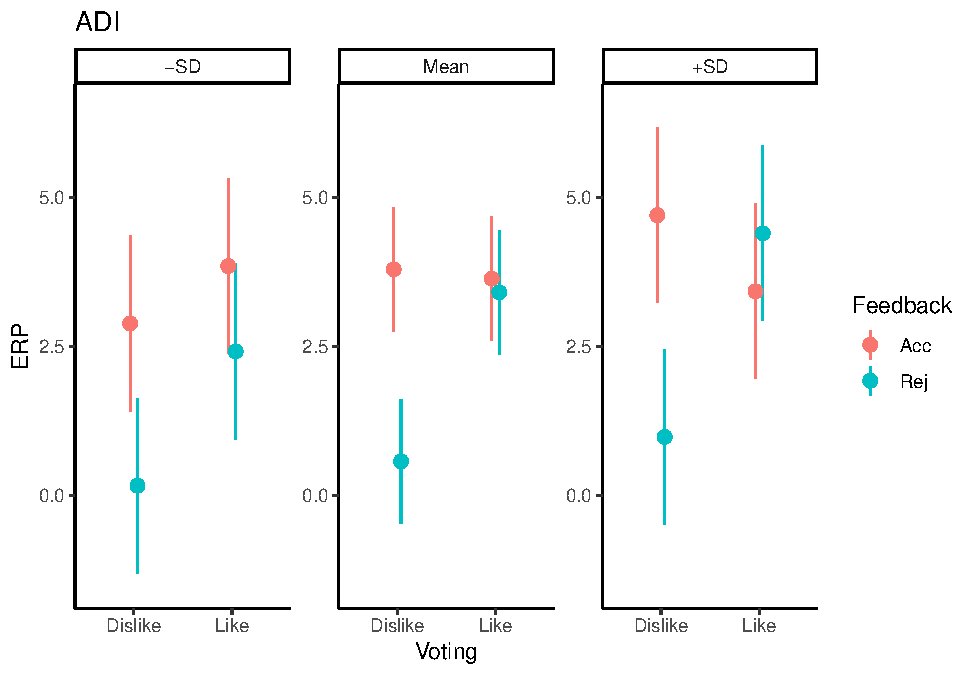
\includegraphics{do01_BUDS_files/figure-latex/unnamed-chunk-17-1.pdf}

\hypertarget{pz}{%
\subsubsection{200-400 Pz}\label{pz}}

\begin{Shaded}
\begin{Highlighting}[]
\NormalTok{models\_200400\_pz\_table }\OtherTok{\textless{}{-}} \FunctionTok{lmer\_adi\_interaction\_table}\NormalTok{(df\_200400\_pz\_long)}
\NormalTok{models\_200400\_pz\_table}\SpecialCharTok{$}\NormalTok{component }\OtherTok{\textless{}{-}} \StringTok{"200400\_pz"}
\end{Highlighting}
\end{Shaded}

\hypertarget{fz}{%
\subsubsection{250-350 Fz}\label{fz}}

\begin{Shaded}
\begin{Highlighting}[]
\FunctionTok{anova}\NormalTok{(}\FunctionTok{lmer}\NormalTok{(}\AttributeTok{formula =}\NormalTok{ ERP }\SpecialCharTok{\textasciitilde{}}\NormalTok{ Feedback}\SpecialCharTok{*}\NormalTok{Voting}\SpecialCharTok{*}\NormalTok{ADI\_NATRANK\_log }\SpecialCharTok{+}\NormalTok{ (}\DecValTok{1} \SpecialCharTok{|}\NormalTok{ ID), }\AttributeTok{data =}\NormalTok{ df\_250450\_fz\_long),}
      \FunctionTok{lmer}\NormalTok{(}\AttributeTok{formula =}\NormalTok{ ERP }\SpecialCharTok{\textasciitilde{}}\NormalTok{ Feedback}\SpecialCharTok{*}\NormalTok{Voting}\SpecialCharTok{*}\NormalTok{ADI\_NATRANK\_log }\SpecialCharTok{+}\NormalTok{ (Feedback }\SpecialCharTok{|}\NormalTok{ ID), }\AttributeTok{data =}\NormalTok{ df\_250450\_fz\_long))}
\FunctionTok{anova}\NormalTok{(}\FunctionTok{lmer}\NormalTok{(}\AttributeTok{formula =}\NormalTok{ ERP }\SpecialCharTok{\textasciitilde{}}\NormalTok{ Feedback}\SpecialCharTok{*}\NormalTok{Voting}\SpecialCharTok{*}\NormalTok{ADI\_NATRANK\_log }\SpecialCharTok{+}\NormalTok{ (}\DecValTok{1} \SpecialCharTok{|}\NormalTok{ ID), }\AttributeTok{data =}\NormalTok{ df\_250450\_fz\_long),}
      \FunctionTok{lmer}\NormalTok{(}\AttributeTok{formula =}\NormalTok{ ERP }\SpecialCharTok{\textasciitilde{}}\NormalTok{ Feedback}\SpecialCharTok{*}\NormalTok{Voting}\SpecialCharTok{*}\NormalTok{ADI\_NATRANK\_log }\SpecialCharTok{+}\NormalTok{ (Voting }\SpecialCharTok{|}\NormalTok{ ID), }\AttributeTok{data =}\NormalTok{ df\_250450\_fz\_long))}

\NormalTok{bbmle}\SpecialCharTok{::}\FunctionTok{AICtab}\NormalTok{(}\FunctionTok{lm}\NormalTok{(}\AttributeTok{formula =}\NormalTok{ ERP }\SpecialCharTok{\textasciitilde{}}\NormalTok{ Feedback}\SpecialCharTok{*}\NormalTok{Voting}\SpecialCharTok{*}\NormalTok{ADI\_NATRANK\_log, }\AttributeTok{data =}\NormalTok{ df\_250450\_fz\_long),}
\NormalTok{      lme4}\SpecialCharTok{::}\FunctionTok{lmer}\NormalTok{(}\AttributeTok{formula =}\NormalTok{ ERP }\SpecialCharTok{\textasciitilde{}}\NormalTok{ Feedback}\SpecialCharTok{*}\NormalTok{Voting}\SpecialCharTok{*}\NormalTok{ADI\_NATRANK\_log }\SpecialCharTok{+}\NormalTok{ (}\DecValTok{1} \SpecialCharTok{|}\NormalTok{ ID), }\AttributeTok{data =}\NormalTok{ df\_250450\_fz\_long, }\AttributeTok{REML=}\ConstantTok{FALSE}\NormalTok{))}

\NormalTok{models\_250450\_fz\_table }\OtherTok{\textless{}{-}} \FunctionTok{lmer\_adi\_interaction\_table}\NormalTok{(df\_250450\_fz\_long)}
\NormalTok{models\_250450\_fz\_table}\SpecialCharTok{$}\NormalTok{component }\OtherTok{\textless{}{-}} \StringTok{"250450\_fz"}

\NormalTok{model\_250450\_fz }\OtherTok{\textless{}{-}} \FunctionTok{lmer}\NormalTok{(}\AttributeTok{formula =}\NormalTok{ ERP }\SpecialCharTok{\textasciitilde{}}\NormalTok{ Feedback}\SpecialCharTok{*}\NormalTok{Voting}\SpecialCharTok{*}\NormalTok{ADI\_NATRANK\_log }\SpecialCharTok{+}\NormalTok{ (}\DecValTok{1} \SpecialCharTok{|}\NormalTok{ ID), }\AttributeTok{data =}\NormalTok{ df\_250450\_fz\_long)}
\FunctionTok{plot\_cap}\NormalTok{(}
\NormalTok{    model\_250450\_fz,}
    \AttributeTok{condition =} \FunctionTok{list}\NormalTok{(}
        \StringTok{"Voting"}\NormalTok{,      }
        \StringTok{"Feedback"}\NormalTok{,}
        \StringTok{"ADI\_NATRANK\_log"} \OtherTok{=} \StringTok{"threenum"}\NormalTok{)) }\SpecialCharTok{+}
  \FunctionTok{scale\_y\_continuous}\NormalTok{(}\AttributeTok{limits=}\FunctionTok{c}\NormalTok{(}\SpecialCharTok{{-}}\DecValTok{3}\NormalTok{,}\DecValTok{5}\NormalTok{)) }\SpecialCharTok{+}
  \FunctionTok{labs}\NormalTok{(}\AttributeTok{title=}\StringTok{"ADI"}\NormalTok{) }\SpecialCharTok{+}
    \FunctionTok{theme\_classic}\NormalTok{()}
\end{Highlighting}
\end{Shaded}

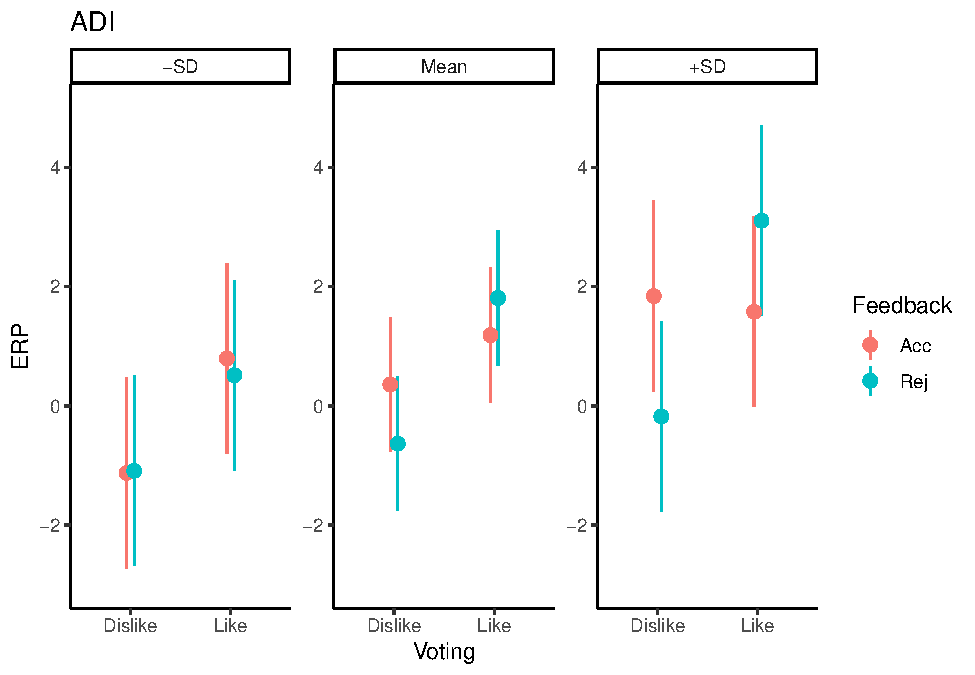
\includegraphics{do01_BUDS_files/figure-latex/unnamed-chunk-19-1.pdf}

\hypertarget{pooled}{%
\subsubsection{275-425 Pooled}\label{pooled}}

\begin{Shaded}
\begin{Highlighting}[]
\NormalTok{models\_275425\_pooled\_table }\OtherTok{\textless{}{-}} \FunctionTok{lmer\_adi\_interaction\_table}\NormalTok{(df\_275425\_pooled\_long)}
\NormalTok{models\_275425\_pooled\_table}\SpecialCharTok{$}\NormalTok{component }\OtherTok{\textless{}{-}} \StringTok{"275425\_pooled"}

\NormalTok{model\_275425\_pooled }\OtherTok{\textless{}{-}} \FunctionTok{lmer}\NormalTok{(}\AttributeTok{formula =}\NormalTok{ ERP }\SpecialCharTok{\textasciitilde{}}\NormalTok{ Feedback}\SpecialCharTok{*}\NormalTok{ADI\_NATRANK\_log }\SpecialCharTok{+}\NormalTok{ (}\DecValTok{1} \SpecialCharTok{|}\NormalTok{ ID), }\AttributeTok{data =} \FunctionTok{filter}\NormalTok{(df\_275425\_pooled\_long, Voting}\SpecialCharTok{==}\StringTok{"Like"}\NormalTok{))}
\FunctionTok{plot\_cap}\NormalTok{(}
\NormalTok{    model\_275425\_pooled,}
    \AttributeTok{condition =} \FunctionTok{list}\NormalTok{(}
      \StringTok{"ADI\_NATRANK\_log"} \OtherTok{=} \StringTok{"threenum"}\NormalTok{,}
        \StringTok{"Feedback"}\NormalTok{)) }\SpecialCharTok{+}
  \CommentTok{\# scale\_y\_continuous(limits=c({-}3,5)) +}
  \FunctionTok{labs}\NormalTok{(}\AttributeTok{title=}\StringTok{"ADI"}\NormalTok{) }\SpecialCharTok{+}
    \FunctionTok{theme\_classic}\NormalTok{()}
\end{Highlighting}
\end{Shaded}

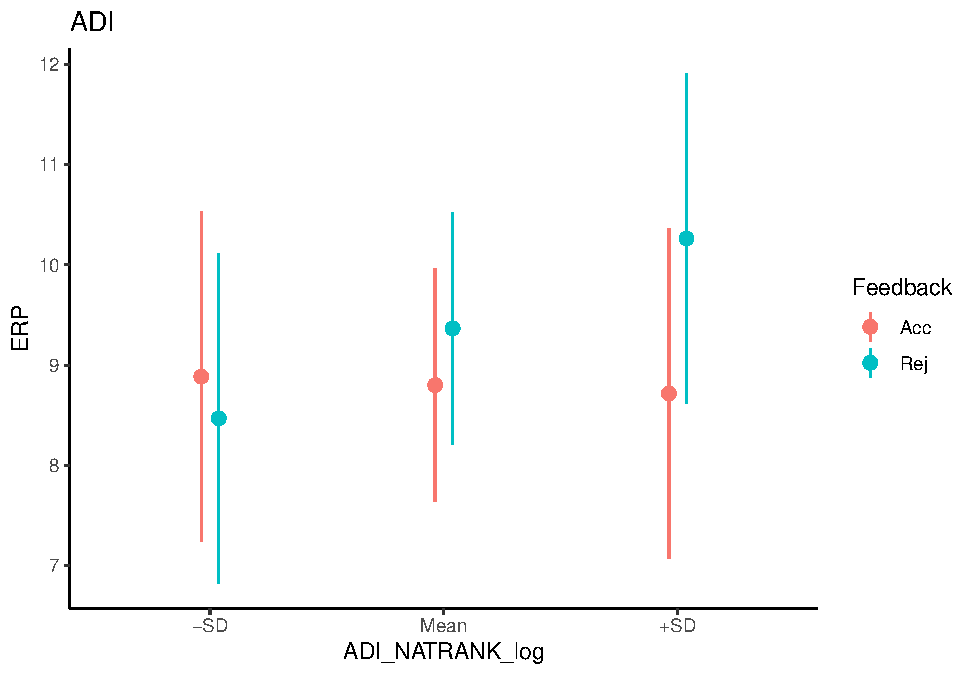
\includegraphics{do01_BUDS_files/figure-latex/unnamed-chunk-20-1.pdf}

\hypertarget{cz-1}{%
\subsubsection{150-275 Cz}\label{cz-1}}

\begin{Shaded}
\begin{Highlighting}[]
\NormalTok{models\_150275\_cz\_table }\OtherTok{\textless{}{-}} \FunctionTok{lmer\_adi\_interaction\_table}\NormalTok{(df\_150275\_cz\_long)}
\NormalTok{models\_150275\_cz\_table}\SpecialCharTok{$}\NormalTok{component }\OtherTok{\textless{}{-}} \StringTok{"150275\_cz"}
\end{Highlighting}
\end{Shaded}

\hypertarget{cz-2}{%
\subsubsection{50-150 Cz}\label{cz-2}}

\begin{Shaded}
\begin{Highlighting}[]
\NormalTok{models\_50150\_cz\_table }\OtherTok{\textless{}{-}} \FunctionTok{lmer\_adi\_interaction\_table}\NormalTok{(df\_50150\_cz\_long)}
\NormalTok{models\_50150\_cz\_table}\SpecialCharTok{$}\NormalTok{component }\OtherTok{\textless{}{-}} \StringTok{"50150\_cz"}
\end{Highlighting}
\end{Shaded}

\hypertarget{all-components}{%
\subsection{All components}\label{all-components}}

\begin{Shaded}
\begin{Highlighting}[]
\NormalTok{models\_table }\OtherTok{\textless{}{-}} \FunctionTok{rbind}\NormalTok{(models\_150275\_cz\_table, models\_50150\_cz\_table, models\_275425\_pooled\_table, models\_250450\_fz\_table, models\_200400\_pz\_table, models\_150350\_cz\_table)}
\NormalTok{models\_table}\SpecialCharTok{$}\NormalTok{p\_fdr }\OtherTok{\textless{}{-}} \FunctionTok{p.adjust}\NormalTok{(models\_table}\SpecialCharTok{$}\NormalTok{p, }\AttributeTok{method=}\StringTok{"fdr"}\NormalTok{)}

\FunctionTok{ggplot}\NormalTok{(models\_table, }\FunctionTok{aes}\NormalTok{(}\AttributeTok{x=}\NormalTok{component, }\AttributeTok{fill=}\NormalTok{model, }\AttributeTok{y=}\FunctionTok{as.numeric}\NormalTok{(p))) }\SpecialCharTok{+}
  \FunctionTok{geom\_col}\NormalTok{(}\AttributeTok{position=}\StringTok{"dodge"}\NormalTok{) }\SpecialCharTok{+}
  \FunctionTok{geom\_hline}\NormalTok{(}\AttributeTok{yintercept=}\FloatTok{0.05}\NormalTok{)}
\end{Highlighting}
\end{Shaded}

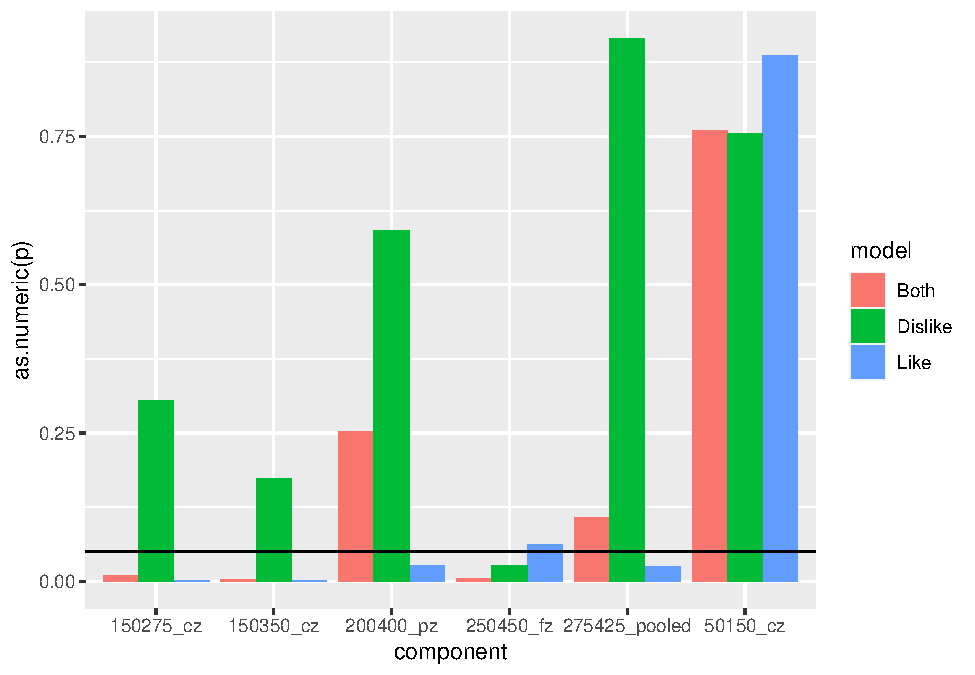
\includegraphics{do01_BUDS_files/figure-latex/unnamed-chunk-23-1.pdf}

\begin{Shaded}
\begin{Highlighting}[]
\FunctionTok{ggplot}\NormalTok{(models\_table, }\FunctionTok{aes}\NormalTok{(}\AttributeTok{x=}\NormalTok{component, }\AttributeTok{fill=}\NormalTok{model, }\AttributeTok{y=}\FunctionTok{as.numeric}\NormalTok{(p\_fdr))) }\SpecialCharTok{+}
  \FunctionTok{geom\_col}\NormalTok{(}\AttributeTok{position=}\StringTok{"dodge"}\NormalTok{) }\SpecialCharTok{+}
  \FunctionTok{geom\_hline}\NormalTok{(}\AttributeTok{yintercept=}\FloatTok{0.05}\NormalTok{)}
\end{Highlighting}
\end{Shaded}

\includegraphics{do01_BUDS_files/figure-latex/unnamed-chunk-23-2.pdf}
Lower ADI is higher SES

\hypertarget{race-and-ethnicity}{%
\subsection{Race and Ethnicity}\label{race-and-ethnicity}}

\begin{Shaded}
\begin{Highlighting}[]
\CommentTok{\# 150{-}350 Cz}
\FunctionTok{summary}\NormalTok{(}\FunctionTok{lmer}\NormalTok{(}\AttributeTok{formula =}\NormalTok{ ERP }\SpecialCharTok{\textasciitilde{}}\NormalTok{ Feedback}\SpecialCharTok{*}\NormalTok{Voting}\SpecialCharTok{*}\NormalTok{Racial\_minority }\SpecialCharTok{+}\NormalTok{ (}\DecValTok{1} \SpecialCharTok{|}\NormalTok{ ID), }\AttributeTok{data =}\NormalTok{ df\_150350\_cz\_long))}
\FunctionTok{summary}\NormalTok{(}\FunctionTok{lmer}\NormalTok{(}\AttributeTok{formula =}\NormalTok{ ERP }\SpecialCharTok{\textasciitilde{}}\NormalTok{ Feedback}\SpecialCharTok{*}\NormalTok{Voting}\SpecialCharTok{*}\NormalTok{Racial\_majority }\SpecialCharTok{+}\NormalTok{ (}\DecValTok{1} \SpecialCharTok{|}\NormalTok{ ID), }\AttributeTok{data =}\NormalTok{ df\_150350\_cz\_long))}
\FunctionTok{summary}\NormalTok{(}\FunctionTok{lmer}\NormalTok{(}\AttributeTok{formula =}\NormalTok{ ERP }\SpecialCharTok{\textasciitilde{}}\NormalTok{ Feedback}\SpecialCharTok{*}\NormalTok{Voting}\SpecialCharTok{*}\NormalTok{demo\_child\_hispanic }\SpecialCharTok{+}\NormalTok{ (}\DecValTok{1} \SpecialCharTok{|}\NormalTok{ ID), }\AttributeTok{data =}\NormalTok{ df\_150350\_cz\_long))}

\CommentTok{\# 200{-}400 Pz}
\FunctionTok{summary}\NormalTok{(}\FunctionTok{lmer}\NormalTok{(}\AttributeTok{formula =}\NormalTok{ ERP }\SpecialCharTok{\textasciitilde{}}\NormalTok{ Feedback}\SpecialCharTok{*}\NormalTok{Voting}\SpecialCharTok{*}\NormalTok{Racial\_minority }\SpecialCharTok{+}\NormalTok{ (}\DecValTok{1} \SpecialCharTok{|}\NormalTok{ ID), }\AttributeTok{data =}\NormalTok{ df\_200400\_pz\_long))}
\FunctionTok{summary}\NormalTok{(}\FunctionTok{lmer}\NormalTok{(}\AttributeTok{formula =}\NormalTok{ ERP }\SpecialCharTok{\textasciitilde{}}\NormalTok{ Feedback}\SpecialCharTok{*}\NormalTok{Voting}\SpecialCharTok{*}\NormalTok{Racial\_majority }\SpecialCharTok{+}\NormalTok{ (}\DecValTok{1} \SpecialCharTok{|}\NormalTok{ ID), }\AttributeTok{data =}\NormalTok{ df\_200400\_pz\_long))}
\FunctionTok{summary}\NormalTok{(}\FunctionTok{lmer}\NormalTok{(}\AttributeTok{formula =}\NormalTok{ ERP }\SpecialCharTok{\textasciitilde{}}\NormalTok{ Feedback}\SpecialCharTok{*}\NormalTok{Voting}\SpecialCharTok{*}\NormalTok{demo\_child\_hispanic }\SpecialCharTok{+}\NormalTok{ (}\DecValTok{1} \SpecialCharTok{|}\NormalTok{ ID), }\AttributeTok{data =}\NormalTok{ df\_200400\_pz\_long))}

\CommentTok{\# 250{-}350 Fz}
\FunctionTok{summary}\NormalTok{(}\FunctionTok{lmer}\NormalTok{(}\AttributeTok{formula =}\NormalTok{ ERP }\SpecialCharTok{\textasciitilde{}}\NormalTok{ Feedback}\SpecialCharTok{*}\NormalTok{Voting}\SpecialCharTok{*}\NormalTok{Racial\_minority }\SpecialCharTok{+}\NormalTok{ (}\DecValTok{1} \SpecialCharTok{|}\NormalTok{ ID), }\AttributeTok{data =}\NormalTok{ df\_250450\_fz\_long))}
\FunctionTok{summary}\NormalTok{(}\FunctionTok{lmer}\NormalTok{(}\AttributeTok{formula =}\NormalTok{ ERP }\SpecialCharTok{\textasciitilde{}}\NormalTok{ Feedback}\SpecialCharTok{*}\NormalTok{Voting}\SpecialCharTok{*}\NormalTok{Racial\_majority }\SpecialCharTok{+}\NormalTok{ (}\DecValTok{1} \SpecialCharTok{|}\NormalTok{ ID), }\AttributeTok{data =}\NormalTok{ df\_250450\_fz\_long))}
\FunctionTok{summary}\NormalTok{(}\FunctionTok{lmer}\NormalTok{(}\AttributeTok{formula =}\NormalTok{ ERP }\SpecialCharTok{\textasciitilde{}}\NormalTok{ Feedback}\SpecialCharTok{*}\NormalTok{Voting}\SpecialCharTok{*}\NormalTok{demo\_child\_hispanic }\SpecialCharTok{+}\NormalTok{ (}\DecValTok{1} \SpecialCharTok{|}\NormalTok{ ID), }\AttributeTok{data =}\NormalTok{ df\_250450\_fz\_long))}

\CommentTok{\# 275{-}425 Fz}
\FunctionTok{summary}\NormalTok{(}\FunctionTok{lmer}\NormalTok{(}\AttributeTok{formula =}\NormalTok{ ERP }\SpecialCharTok{\textasciitilde{}}\NormalTok{ Feedback}\SpecialCharTok{*}\NormalTok{Voting}\SpecialCharTok{*}\NormalTok{Racial\_minority }\SpecialCharTok{+}\NormalTok{ (}\DecValTok{1} \SpecialCharTok{|}\NormalTok{ ID), }\AttributeTok{data =}\NormalTok{ df\_275425\_pooled\_long))}
\FunctionTok{summary}\NormalTok{(}\FunctionTok{lmer}\NormalTok{(}\AttributeTok{formula =}\NormalTok{ ERP }\SpecialCharTok{\textasciitilde{}}\NormalTok{ Feedback}\SpecialCharTok{*}\NormalTok{Voting}\SpecialCharTok{*}\NormalTok{Racial\_majority }\SpecialCharTok{+}\NormalTok{ (}\DecValTok{1} \SpecialCharTok{|}\NormalTok{ ID), }\AttributeTok{data =}\NormalTok{ df\_275425\_pooled\_long))}
\FunctionTok{summary}\NormalTok{(}\FunctionTok{lmer}\NormalTok{(}\AttributeTok{formula =}\NormalTok{ ERP }\SpecialCharTok{\textasciitilde{}}\NormalTok{ Feedback}\SpecialCharTok{*}\NormalTok{Voting}\SpecialCharTok{*}\NormalTok{demo\_child\_hispanic }\SpecialCharTok{+}\NormalTok{ (}\DecValTok{1} \SpecialCharTok{|}\NormalTok{ ID), }\AttributeTok{data =}\NormalTok{ df\_275425\_pooled\_long))}
\end{Highlighting}
\end{Shaded}

\hypertarget{covaring-for-age-sex-hispanic-stress-idas}{%
\subsection{Covaring for age, sex, hispanic, stress,
IDAS}\label{covaring-for-age-sex-hispanic-stress-idas}}

\begin{Shaded}
\begin{Highlighting}[]
\NormalTok{lmer\_adi\_interaction\_table\_cov }\OtherTok{\textless{}{-}} \ControlFlowTok{function}\NormalTok{(data, Component) \{}
\NormalTok{  new\_model }\OtherTok{\textless{}{-}} \FunctionTok{data.frame}\NormalTok{(}\AttributeTok{model =} \FunctionTok{c}\NormalTok{(}\StringTok{"Both"}\NormalTok{,}\StringTok{"Like"}\NormalTok{,}\StringTok{"Dislike"}\NormalTok{),}
                            \AttributeTok{beta =} \ConstantTok{NA}\NormalTok{, }
                            \AttributeTok{p =} \ConstantTok{NA}\NormalTok{,}
                          \AttributeTok{component =}\NormalTok{ Component)}
\NormalTok{new\_model}\SpecialCharTok{$}\NormalTok{beta }\OtherTok{\textless{}{-}} \FunctionTok{c}\NormalTok{(broom.mixed}\SpecialCharTok{::}\FunctionTok{tidy}\NormalTok{(}\FunctionTok{lmer}\NormalTok{(}\AttributeTok{formula =}\NormalTok{ ERP }\SpecialCharTok{\textasciitilde{}}\NormalTok{ Feedback}\SpecialCharTok{*}\NormalTok{Voting}\SpecialCharTok{*}\NormalTok{ADI\_NATRANK\_log\_z }\SpecialCharTok{+}\NormalTok{ Age }\SpecialCharTok{+}\NormalTok{ Sex }\SpecialCharTok{+}\NormalTok{ demo\_child\_hispanic }\SpecialCharTok{+}\NormalTok{ StressCT }\SpecialCharTok{+}\NormalTok{ StressTH }\SpecialCharTok{+}\NormalTok{ IDAS\_depression }\SpecialCharTok{+}\NormalTok{  (}\DecValTok{1} \SpecialCharTok{|}\NormalTok{ ID), }\AttributeTok{data =}\NormalTok{ data))[}\DecValTok{14}\NormalTok{,}\DecValTok{4}\NormalTok{], }
\NormalTok{                    broom.mixed}\SpecialCharTok{::}\FunctionTok{tidy}\NormalTok{(}\FunctionTok{lmer}\NormalTok{(}\AttributeTok{formula =}\NormalTok{ ERP }\SpecialCharTok{\textasciitilde{}}\NormalTok{ Feedback}\SpecialCharTok{*}\NormalTok{ADI\_NATRANK\_log\_z }\SpecialCharTok{+}\NormalTok{ Age }\SpecialCharTok{+}\NormalTok{ Sex }\SpecialCharTok{+}\NormalTok{ demo\_child\_hispanic }\SpecialCharTok{+}\NormalTok{ StressCT }\SpecialCharTok{+}\NormalTok{ StressTH }\SpecialCharTok{+}\NormalTok{ IDAS\_depression }\SpecialCharTok{+}\NormalTok{ (}\DecValTok{1} \SpecialCharTok{|}\NormalTok{ ID), }\AttributeTok{data =} \FunctionTok{filter}\NormalTok{(data, Voting}\SpecialCharTok{==}\StringTok{"Like"}\NormalTok{)))[}\DecValTok{10}\NormalTok{,}\DecValTok{4}\NormalTok{],}
\NormalTok{                    broom.mixed}\SpecialCharTok{::}\FunctionTok{tidy}\NormalTok{(}\FunctionTok{lmer}\NormalTok{(}\AttributeTok{formula =}\NormalTok{ ERP }\SpecialCharTok{\textasciitilde{}}\NormalTok{ Feedback}\SpecialCharTok{*}\NormalTok{ADI\_NATRANK\_log\_z }\SpecialCharTok{+}\NormalTok{ Age }\SpecialCharTok{+}\NormalTok{ Sex }\SpecialCharTok{+}\NormalTok{ demo\_child\_hispanic }\SpecialCharTok{+}\NormalTok{ StressCT }\SpecialCharTok{+}\NormalTok{ StressTH }\SpecialCharTok{+}\NormalTok{ IDAS\_depression }\SpecialCharTok{+}\NormalTok{  (}\DecValTok{1} \SpecialCharTok{|}\NormalTok{ ID), }\AttributeTok{data =} \FunctionTok{filter}\NormalTok{(data, Voting}\SpecialCharTok{==}\StringTok{"Dislike"}\NormalTok{)))[}\DecValTok{10}\NormalTok{,}\DecValTok{4}\NormalTok{])}

\NormalTok{new\_model}\SpecialCharTok{$}\NormalTok{p }\OtherTok{\textless{}{-}} \FunctionTok{c}\NormalTok{(broom.mixed}\SpecialCharTok{::}\FunctionTok{tidy}\NormalTok{(}\FunctionTok{lmer}\NormalTok{(}\AttributeTok{formula =}\NormalTok{ ERP }\SpecialCharTok{\textasciitilde{}}\NormalTok{ Feedback}\SpecialCharTok{*}\NormalTok{Voting}\SpecialCharTok{*}\NormalTok{ADI\_NATRANK\_log\_z }\SpecialCharTok{+}\NormalTok{ Age }\SpecialCharTok{+}\NormalTok{ Sex }\SpecialCharTok{+}\NormalTok{ demo\_child\_hispanic }\SpecialCharTok{+}\NormalTok{ StressCT }\SpecialCharTok{+}\NormalTok{ StressTH }\SpecialCharTok{+}\NormalTok{ IDAS\_depression }\SpecialCharTok{+}\NormalTok{ (}\DecValTok{1} \SpecialCharTok{|}\NormalTok{ ID), }\AttributeTok{data =}\NormalTok{ data))[}\DecValTok{14}\NormalTok{,}\DecValTok{8}\NormalTok{], }
\NormalTok{                    broom.mixed}\SpecialCharTok{::}\FunctionTok{tidy}\NormalTok{(}\FunctionTok{lmer}\NormalTok{(}\AttributeTok{formula =}\NormalTok{ ERP }\SpecialCharTok{\textasciitilde{}}\NormalTok{ Feedback}\SpecialCharTok{*}\NormalTok{ADI\_NATRANK\_log\_z }\SpecialCharTok{+}\NormalTok{ Age }\SpecialCharTok{+}\NormalTok{ Sex }\SpecialCharTok{+}\NormalTok{ demo\_child\_hispanic }\SpecialCharTok{+}\NormalTok{ StressCT }\SpecialCharTok{+}\NormalTok{ StressTH }\SpecialCharTok{+}\NormalTok{ IDAS\_depression }\SpecialCharTok{+}\NormalTok{ (}\DecValTok{1} \SpecialCharTok{|}\NormalTok{ ID), }\AttributeTok{data =} \FunctionTok{filter}\NormalTok{(data, Voting}\SpecialCharTok{==}\StringTok{"Like"}\NormalTok{)))[}\DecValTok{10}\NormalTok{,}\DecValTok{8}\NormalTok{],}
\NormalTok{                    broom.mixed}\SpecialCharTok{::}\FunctionTok{tidy}\NormalTok{(}\FunctionTok{lmer}\NormalTok{(}\AttributeTok{formula =}\NormalTok{ ERP }\SpecialCharTok{\textasciitilde{}}\NormalTok{ Feedback}\SpecialCharTok{*}\NormalTok{ADI\_NATRANK\_log\_z }\SpecialCharTok{+}\NormalTok{ Age }\SpecialCharTok{+}\NormalTok{ Sex }\SpecialCharTok{+}\NormalTok{ demo\_child\_hispanic }\SpecialCharTok{+}\NormalTok{ StressCT }\SpecialCharTok{+}\NormalTok{ StressTH }\SpecialCharTok{+}\NormalTok{ IDAS\_depression }\SpecialCharTok{+}\NormalTok{ (}\DecValTok{1} \SpecialCharTok{|}\NormalTok{ ID), }\AttributeTok{data =} \FunctionTok{filter}\NormalTok{(data, Voting}\SpecialCharTok{==}\StringTok{"Dislike"}\NormalTok{)))[}\DecValTok{10}\NormalTok{,}\DecValTok{8}\NormalTok{])}
\NormalTok{new\_model}
\NormalTok{\}}

\NormalTok{models\_table\_cov }\OtherTok{\textless{}{-}} \FunctionTok{rbind}\NormalTok{(}\FunctionTok{lmer\_adi\_interaction\_table\_cov}\NormalTok{(df\_150275\_cz\_long\_strain, }\StringTok{"150275\_cz"}\NormalTok{),}
        \FunctionTok{lmer\_adi\_interaction\_table\_cov}\NormalTok{(df\_50150\_cz\_long\_strain, }\StringTok{"50150\_cz"}\NormalTok{),}
        \FunctionTok{lmer\_adi\_interaction\_table\_cov}\NormalTok{(df\_275425\_cz\_long\_strain, }\StringTok{"275425\_cz"}\NormalTok{),}
        \FunctionTok{lmer\_adi\_interaction\_table\_cov}\NormalTok{(df\_275425\_pooled\_long\_strain, }\StringTok{"275425\_pooled"}\NormalTok{),}
        \FunctionTok{lmer\_adi\_interaction\_table\_cov}\NormalTok{(df\_250450\_fz\_long\_strain, }\StringTok{"250450\_fz"}\NormalTok{),}
        \FunctionTok{lmer\_adi\_interaction\_table\_cov}\NormalTok{(df\_200400\_pz\_long\_strain, }\StringTok{"200400\_pz"}\NormalTok{),}
        \FunctionTok{lmer\_adi\_interaction\_table\_cov}\NormalTok{(df\_150350\_cz\_long\_strain, }\StringTok{"150350\_cz"}\NormalTok{))}
\NormalTok{models\_table\_cov}\SpecialCharTok{$}\NormalTok{p\_fdr }\OtherTok{\textless{}{-}} \FunctionTok{p.adjust}\NormalTok{(models\_table\_cov}\SpecialCharTok{$}\NormalTok{p, }\AttributeTok{method=}\StringTok{"fdr"}\NormalTok{)}

\FunctionTok{ggplot}\NormalTok{(models\_table\_cov, }\FunctionTok{aes}\NormalTok{(}\AttributeTok{x=}\NormalTok{component, }\AttributeTok{fill=}\NormalTok{model, }\AttributeTok{y=}\FunctionTok{as.numeric}\NormalTok{(p))) }\SpecialCharTok{+}
  \FunctionTok{geom\_col}\NormalTok{(}\AttributeTok{position=}\StringTok{"dodge"}\NormalTok{) }\SpecialCharTok{+}
  \FunctionTok{geom\_hline}\NormalTok{(}\AttributeTok{yintercept=}\FloatTok{0.05}\NormalTok{)}
\end{Highlighting}
\end{Shaded}

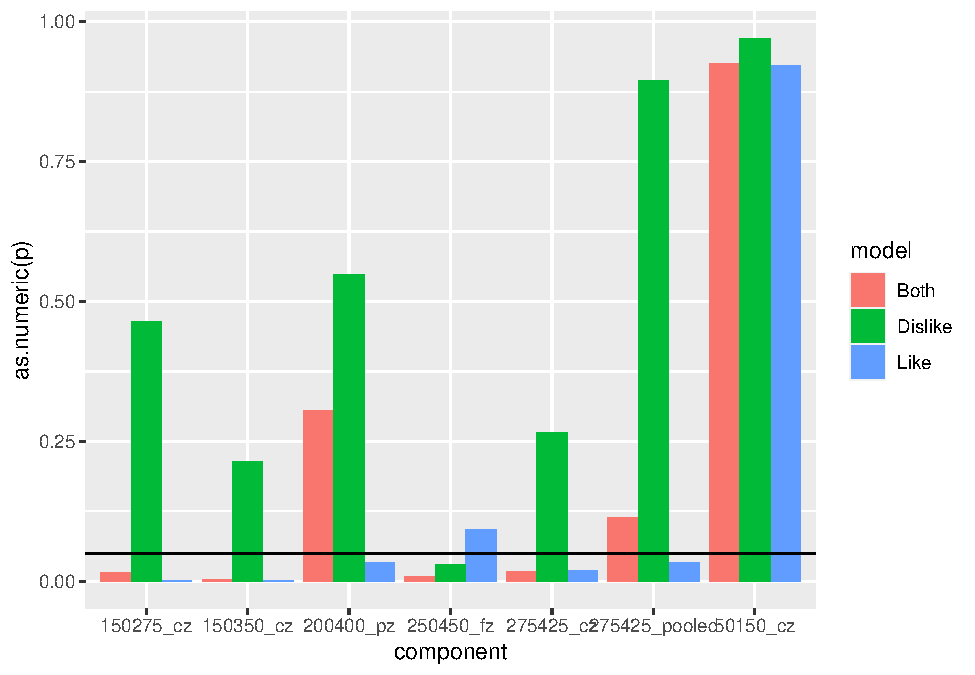
\includegraphics{do01_BUDS_files/figure-latex/unnamed-chunk-25-1.pdf}

\begin{Shaded}
\begin{Highlighting}[]
\FunctionTok{ggplot}\NormalTok{(models\_table\_cov, }\FunctionTok{aes}\NormalTok{(}\AttributeTok{x=}\NormalTok{component, }\AttributeTok{fill=}\NormalTok{model, }\AttributeTok{y=}\FunctionTok{as.numeric}\NormalTok{(p\_fdr))) }\SpecialCharTok{+}
  \FunctionTok{geom\_col}\NormalTok{(}\AttributeTok{position=}\StringTok{"dodge"}\NormalTok{) }\SpecialCharTok{+}
  \FunctionTok{geom\_hline}\NormalTok{(}\AttributeTok{yintercept=}\FloatTok{0.05}\NormalTok{)}
\end{Highlighting}
\end{Shaded}

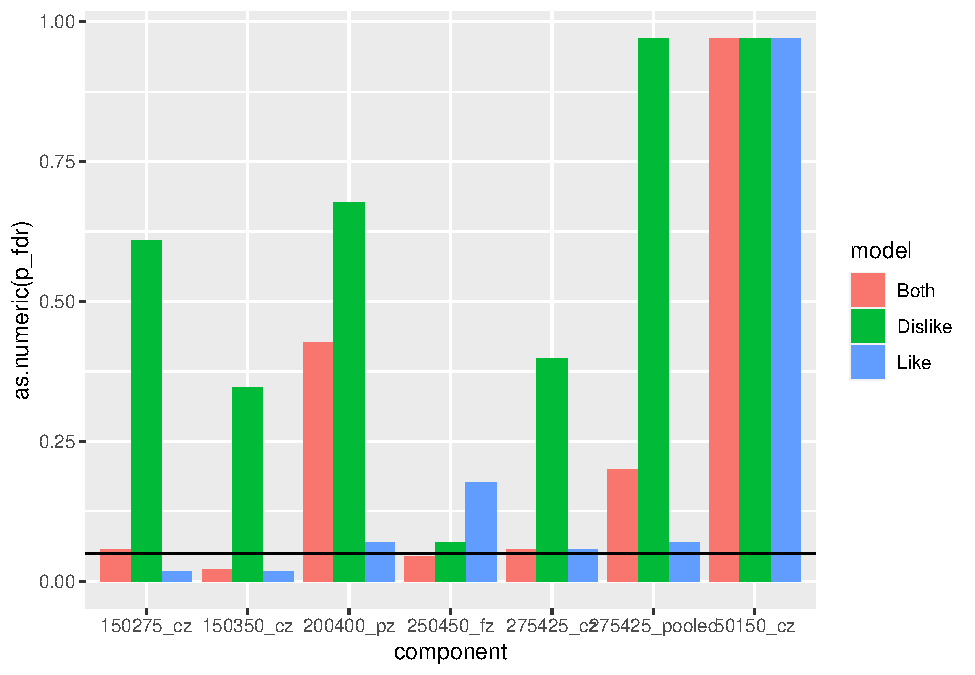
\includegraphics{do01_BUDS_files/figure-latex/unnamed-chunk-25-2.pdf}

\hypertarget{exaggerated-response-to-rejection}{%
\section{Exaggerated response to
rejection}\label{exaggerated-response-to-rejection}}

\begin{Shaded}
\begin{Highlighting}[]
\FunctionTok{ggplot}\NormalTok{(}\AttributeTok{data=}\FunctionTok{filter}\NormalTok{(df\_ga\_Cz\_adi\_wide, Condition}\SpecialCharTok{==}\StringTok{"Acc\_Acc"} \SpecialCharTok{|}\NormalTok{ Condition}\SpecialCharTok{==}\StringTok{"Acc\_Rej"}\NormalTok{), }\FunctionTok{aes}\NormalTok{(}\AttributeTok{x=}\NormalTok{Time, }\AttributeTok{y=}\NormalTok{grand\_average, }\AttributeTok{color=}\NormalTok{adi\_median\_split)) }\SpecialCharTok{+}
  \FunctionTok{facet\_wrap}\NormalTok{(}\SpecialCharTok{\textasciitilde{}}\NormalTok{ Condition) }\SpecialCharTok{+}
  \FunctionTok{xlim}\NormalTok{(}\SpecialCharTok{{-}}\DecValTok{200}\NormalTok{, }\DecValTok{800}\NormalTok{) }\SpecialCharTok{+}
  \FunctionTok{ylim}\NormalTok{( }\SpecialCharTok{{-}}\DecValTok{5}\NormalTok{, }\DecValTok{13}\NormalTok{) }\SpecialCharTok{+}
  \FunctionTok{geom\_line}\NormalTok{(}\AttributeTok{linewidth=}\DecValTok{1}\NormalTok{) }\SpecialCharTok{+}
  \FunctionTok{annotate}\NormalTok{(}\StringTok{"rect"}\NormalTok{, }\AttributeTok{xmin=}\DecValTok{150}\NormalTok{, }\AttributeTok{xmax=}\DecValTok{350}\NormalTok{, }\AttributeTok{ymin=}\DecValTok{0}\NormalTok{, }\AttributeTok{ymax=}\ConstantTok{Inf}\NormalTok{, }\AttributeTok{alpha=}\FloatTok{0.2}\NormalTok{, }\AttributeTok{fill=}\StringTok{"red"}\NormalTok{) }\SpecialCharTok{+}
  \FunctionTok{geom\_rect}\NormalTok{(}\FunctionTok{aes}\NormalTok{(}\AttributeTok{xmin=}\DecValTok{0}\NormalTok{, }\AttributeTok{xmax=}\DecValTok{0}\NormalTok{, }\AttributeTok{ymin=}\SpecialCharTok{{-}}\DecValTok{5}\NormalTok{, }\AttributeTok{ymax=}\DecValTok{12}\NormalTok{), }\AttributeTok{color=}\StringTok{"black"}\NormalTok{) }\SpecialCharTok{+}
  \FunctionTok{geom\_rect}\NormalTok{(}\FunctionTok{aes}\NormalTok{(}\AttributeTok{xmin=}\SpecialCharTok{{-}}\DecValTok{200}\NormalTok{, }\AttributeTok{xmax=}\DecValTok{800}\NormalTok{, }\AttributeTok{ymin=}\DecValTok{0}\NormalTok{, }\AttributeTok{ymax=}\DecValTok{0}\NormalTok{), }\AttributeTok{color=}\StringTok{"black"}\NormalTok{) }\SpecialCharTok{+}
  \FunctionTok{labs}\NormalTok{(}\AttributeTok{x=}\StringTok{"Time (ms)"}\NormalTok{, }\AttributeTok{y=}\StringTok{"Cz"}\NormalTok{, }\AttributeTok{title=}\StringTok{"High value peers"}\NormalTok{) }\SpecialCharTok{+}
  \FunctionTok{theme\_apa}\NormalTok{(}\AttributeTok{base\_size =} \DecValTok{12}\NormalTok{) }\SpecialCharTok{+} \FunctionTok{theme}\NormalTok{(}\AttributeTok{legend.position=}\StringTok{"top"}\NormalTok{)}
\end{Highlighting}
\end{Shaded}

\begin{verbatim}
## Warning: Removed 1198 rows containing missing values (`geom_line()`).
\end{verbatim}

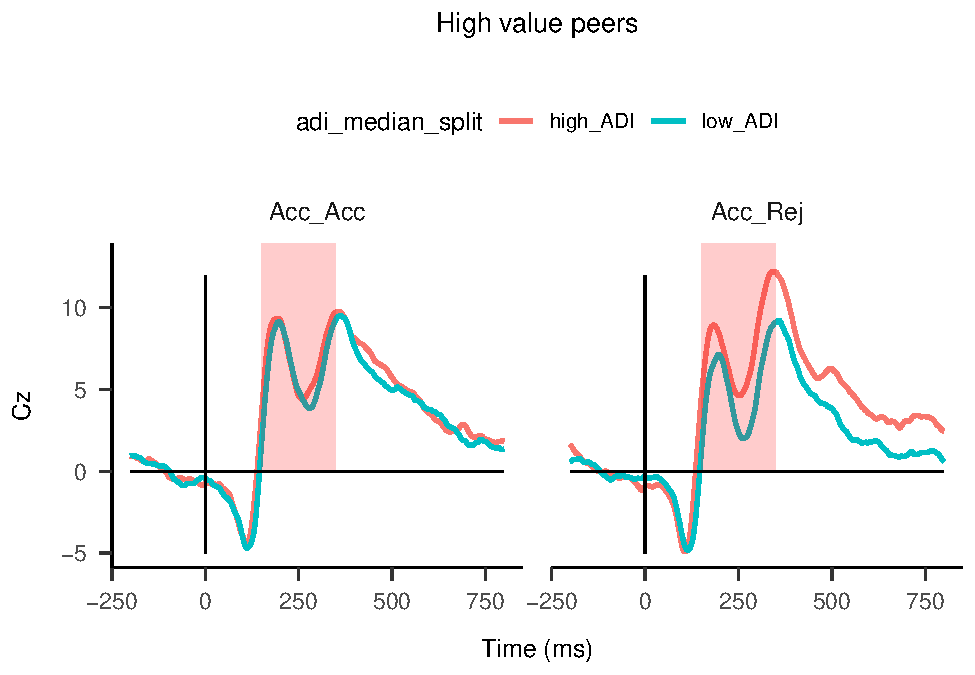
\includegraphics{do01_BUDS_files/figure-latex/unnamed-chunk-26-1.pdf}

\begin{Shaded}
\begin{Highlighting}[]
\FunctionTok{ggplot}\NormalTok{(}\AttributeTok{data=}\FunctionTok{filter}\NormalTok{(df\_ga\_Fz\_adi\_wide, Condition}\SpecialCharTok{==}\StringTok{"Acc\_Acc"} \SpecialCharTok{|}\NormalTok{ Condition}\SpecialCharTok{==}\StringTok{"Acc\_Rej"}\NormalTok{), }\FunctionTok{aes}\NormalTok{(}\AttributeTok{x=}\NormalTok{Time, }\AttributeTok{y=}\NormalTok{grand\_average, }\AttributeTok{color=}\NormalTok{adi\_median\_split)) }\SpecialCharTok{+}
  \FunctionTok{facet\_wrap}\NormalTok{(}\SpecialCharTok{\textasciitilde{}}\NormalTok{ Condition) }\SpecialCharTok{+}
  \FunctionTok{xlim}\NormalTok{(}\SpecialCharTok{{-}}\DecValTok{200}\NormalTok{, }\DecValTok{800}\NormalTok{) }\SpecialCharTok{+}
  \FunctionTok{ylim}\NormalTok{( }\SpecialCharTok{{-}}\DecValTok{5}\NormalTok{, }\DecValTok{13}\NormalTok{) }\SpecialCharTok{+}
  \FunctionTok{geom\_line}\NormalTok{(}\AttributeTok{linewidth=}\DecValTok{1}\NormalTok{) }\SpecialCharTok{+}
  \FunctionTok{annotate}\NormalTok{(}\StringTok{"rect"}\NormalTok{, }\AttributeTok{xmin=}\DecValTok{250}\NormalTok{, }\AttributeTok{xmax=}\DecValTok{450}\NormalTok{, }\AttributeTok{ymin=}\DecValTok{0}\NormalTok{, }\AttributeTok{ymax=}\ConstantTok{Inf}\NormalTok{, }\AttributeTok{alpha=}\FloatTok{0.2}\NormalTok{, }\AttributeTok{fill=}\StringTok{"red"}\NormalTok{) }\SpecialCharTok{+}
  \FunctionTok{geom\_rect}\NormalTok{(}\FunctionTok{aes}\NormalTok{(}\AttributeTok{xmin=}\DecValTok{0}\NormalTok{, }\AttributeTok{xmax=}\DecValTok{0}\NormalTok{, }\AttributeTok{ymin=}\SpecialCharTok{{-}}\DecValTok{5}\NormalTok{, }\AttributeTok{ymax=}\DecValTok{12}\NormalTok{), }\AttributeTok{color=}\StringTok{"black"}\NormalTok{) }\SpecialCharTok{+}
  \FunctionTok{geom\_rect}\NormalTok{(}\FunctionTok{aes}\NormalTok{(}\AttributeTok{xmin=}\SpecialCharTok{{-}}\DecValTok{200}\NormalTok{, }\AttributeTok{xmax=}\DecValTok{800}\NormalTok{, }\AttributeTok{ymin=}\DecValTok{0}\NormalTok{, }\AttributeTok{ymax=}\DecValTok{0}\NormalTok{), }\AttributeTok{color=}\StringTok{"black"}\NormalTok{) }\SpecialCharTok{+}
  \FunctionTok{labs}\NormalTok{(}\AttributeTok{x=}\StringTok{"Time (ms)"}\NormalTok{, }\AttributeTok{y=}\StringTok{"Fz"}\NormalTok{, }\AttributeTok{title=}\StringTok{"High value peers"}\NormalTok{) }\SpecialCharTok{+}
  \FunctionTok{theme\_apa}\NormalTok{(}\AttributeTok{base\_size =} \DecValTok{12}\NormalTok{) }\SpecialCharTok{+} \FunctionTok{theme}\NormalTok{(}\AttributeTok{legend.position=}\StringTok{"top"}\NormalTok{)}
\end{Highlighting}
\end{Shaded}

\begin{verbatim}
## Warning: Removed 1198 rows containing missing values (`geom_line()`).
\end{verbatim}

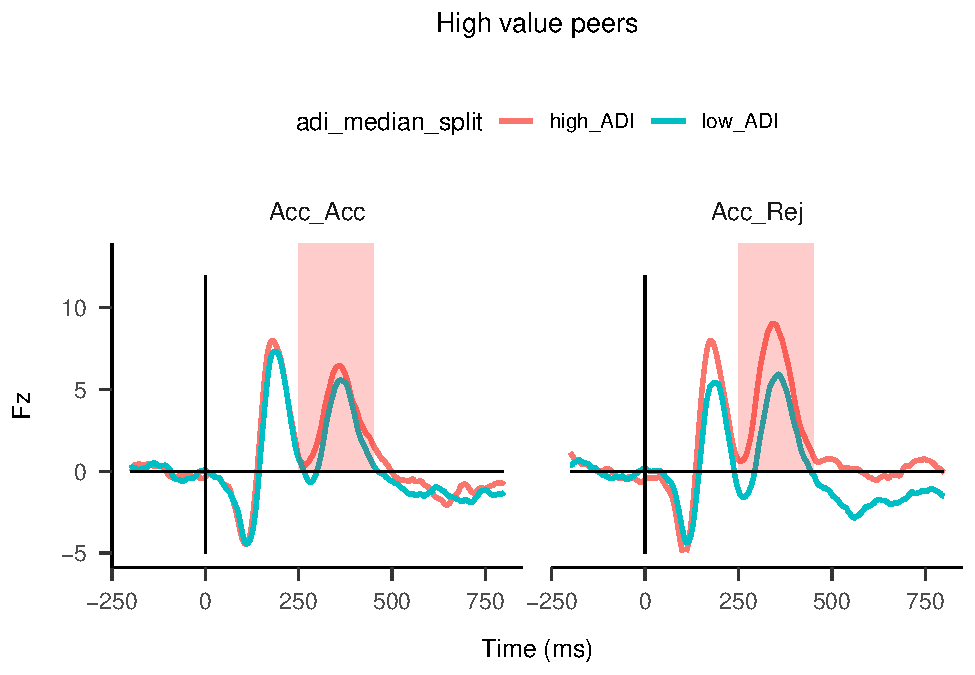
\includegraphics{do01_BUDS_files/figure-latex/unnamed-chunk-26-2.pdf}

\begin{Shaded}
\begin{Highlighting}[]
\FunctionTok{ggplot}\NormalTok{(}\AttributeTok{data=}\FunctionTok{filter}\NormalTok{(df\_ga\_Pz\_adi\_wide, Condition}\SpecialCharTok{==}\StringTok{"Acc\_Acc"} \SpecialCharTok{|}\NormalTok{ Condition}\SpecialCharTok{==}\StringTok{"Acc\_Rej"}\NormalTok{), }\FunctionTok{aes}\NormalTok{(}\AttributeTok{x=}\NormalTok{Time, }\AttributeTok{y=}\NormalTok{grand\_average, }\AttributeTok{color=}\NormalTok{adi\_median\_split)) }\SpecialCharTok{+}
  \FunctionTok{facet\_wrap}\NormalTok{(}\SpecialCharTok{\textasciitilde{}}\NormalTok{ Condition) }\SpecialCharTok{+}
  \FunctionTok{xlim}\NormalTok{(}\SpecialCharTok{{-}}\DecValTok{200}\NormalTok{, }\DecValTok{800}\NormalTok{) }\SpecialCharTok{+}
  \FunctionTok{ylim}\NormalTok{( }\SpecialCharTok{{-}}\DecValTok{5}\NormalTok{, }\DecValTok{15}\NormalTok{) }\SpecialCharTok{+}
  \FunctionTok{geom\_line}\NormalTok{(}\AttributeTok{linewidth=}\DecValTok{1}\NormalTok{) }\SpecialCharTok{+}
  \FunctionTok{annotate}\NormalTok{(}\StringTok{"rect"}\NormalTok{, }\AttributeTok{xmin=}\DecValTok{200}\NormalTok{, }\AttributeTok{xmax=}\DecValTok{400}\NormalTok{, }\AttributeTok{ymin=}\DecValTok{0}\NormalTok{, }\AttributeTok{ymax=}\ConstantTok{Inf}\NormalTok{, }\AttributeTok{alpha=}\FloatTok{0.2}\NormalTok{, }\AttributeTok{fill=}\StringTok{"red"}\NormalTok{) }\SpecialCharTok{+}
  \FunctionTok{geom\_rect}\NormalTok{(}\FunctionTok{aes}\NormalTok{(}\AttributeTok{xmin=}\DecValTok{0}\NormalTok{, }\AttributeTok{xmax=}\DecValTok{0}\NormalTok{, }\AttributeTok{ymin=}\SpecialCharTok{{-}}\DecValTok{5}\NormalTok{, }\AttributeTok{ymax=}\DecValTok{12}\NormalTok{), }\AttributeTok{color=}\StringTok{"black"}\NormalTok{) }\SpecialCharTok{+}
  \FunctionTok{geom\_rect}\NormalTok{(}\FunctionTok{aes}\NormalTok{(}\AttributeTok{xmin=}\SpecialCharTok{{-}}\DecValTok{200}\NormalTok{, }\AttributeTok{xmax=}\DecValTok{800}\NormalTok{, }\AttributeTok{ymin=}\DecValTok{0}\NormalTok{, }\AttributeTok{ymax=}\DecValTok{0}\NormalTok{), }\AttributeTok{color=}\StringTok{"black"}\NormalTok{) }\SpecialCharTok{+}
  \FunctionTok{labs}\NormalTok{(}\AttributeTok{x=}\StringTok{"Time (ms)"}\NormalTok{, }\AttributeTok{y=}\StringTok{"Pz"}\NormalTok{, }\AttributeTok{title=}\StringTok{"High value peers"}\NormalTok{) }\SpecialCharTok{+}
  \FunctionTok{theme\_apa}\NormalTok{(}\AttributeTok{base\_size =} \DecValTok{12}\NormalTok{) }\SpecialCharTok{+} \FunctionTok{theme}\NormalTok{(}\AttributeTok{legend.position=}\StringTok{"top"}\NormalTok{)}
\end{Highlighting}
\end{Shaded}

\begin{verbatim}
## Warning: Removed 1198 rows containing missing values (`geom_line()`).
\end{verbatim}

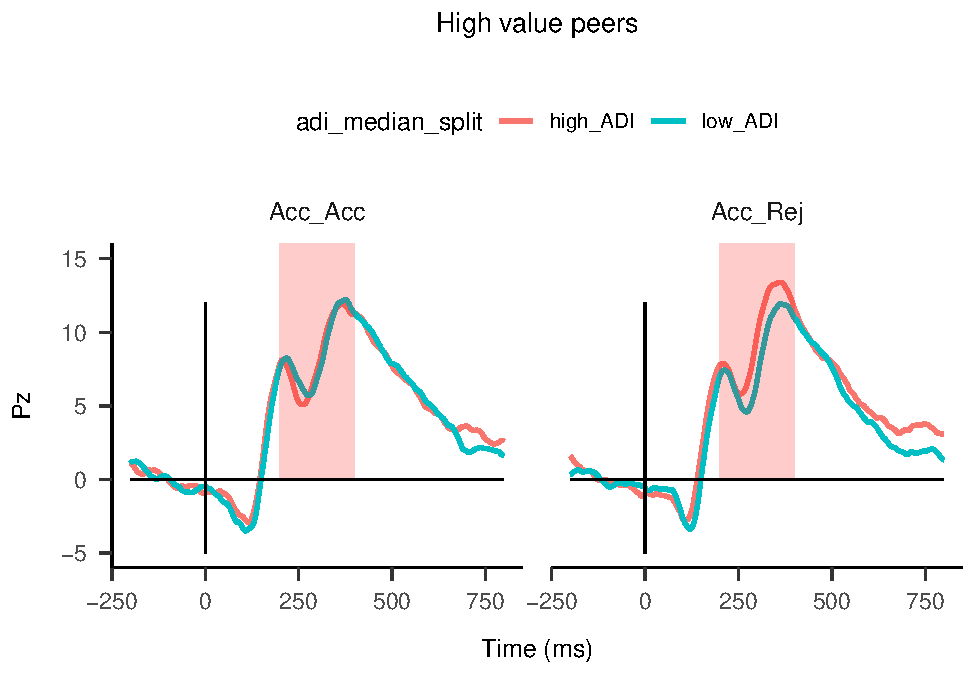
\includegraphics{do01_BUDS_files/figure-latex/unnamed-chunk-26-3.pdf}

\hypertarget{section}{%
\section{``\,''}\label{section}}

\hypertarget{section-1}{%
\section{``\,''}\label{section-1}}

\hypertarget{section-2}{%
\section{``\,''}\label{section-2}}

\hypertarget{regressions-with-addi}{%
\section{Regressions with ADDI}\label{regressions-with-addi}}

\begin{Shaded}
\begin{Highlighting}[]
\ControlFlowTok{for}\NormalTok{ (p }\ControlFlowTok{in} \FunctionTok{c}\NormalTok{(}\StringTok{"addi\_total"}\NormalTok{,}\StringTok{"addi\_01"}\NormalTok{,}\StringTok{"addi\_educ"}\NormalTok{,}\StringTok{"addi\_instit"}\NormalTok{,}\StringTok{"addi\_distress"}\NormalTok{)) \{}
      \FunctionTok{eval}\NormalTok{(}\FunctionTok{parse}\NormalTok{(}\AttributeTok{text=}\FunctionTok{paste0}\NormalTok{(}\StringTok{\textquotesingle{}hist(df\_150350\_cz$\textquotesingle{}}\NormalTok{,p,}\StringTok{\textquotesingle{})\textquotesingle{}}\NormalTok{)))}
\NormalTok{    \}}
\FunctionTok{table}\NormalTok{(df\_150350\_cz}\SpecialCharTok{$}\NormalTok{addi\_instit}\SpecialCharTok{\textgreater{}}\DecValTok{0}\NormalTok{)}

\ControlFlowTok{for}\NormalTok{ (data }\ControlFlowTok{in} \FunctionTok{c}\NormalTok{(}\StringTok{"df\_150350\_cz"}\NormalTok{,}\StringTok{"df\_250450\_fz"}\NormalTok{,}\StringTok{"df\_200400\_pz"}\NormalTok{)) \{}
  \ControlFlowTok{for}\NormalTok{ (comp }\ControlFlowTok{in} \FunctionTok{c}\NormalTok{(}\StringTok{"A\_all"}\NormalTok{,}\StringTok{"AA\_AR"}\NormalTok{,}\StringTok{"RA\_RR"}\NormalTok{)) \{}
    \ControlFlowTok{for}\NormalTok{ (p }\ControlFlowTok{in} \FunctionTok{c}\NormalTok{(}\StringTok{"addi\_total"}\NormalTok{,}\StringTok{"addi\_01"}\NormalTok{,}\StringTok{"addi\_educ"}\NormalTok{,}\StringTok{"addi\_instit"}\NormalTok{,}\StringTok{"addi\_distress"}\NormalTok{)) \{}
      \FunctionTok{eval}\NormalTok{(}\FunctionTok{parse}\NormalTok{(}\AttributeTok{text=}\FunctionTok{paste0}\NormalTok{(}\StringTok{\textquotesingle{}print(zeroinfl(\textquotesingle{}}\NormalTok{,p,}\StringTok{\textquotesingle{} \textasciitilde{} \textquotesingle{}}\NormalTok{,comp,}\StringTok{\textquotesingle{}, \textquotesingle{}}\NormalTok{,data,}\StringTok{\textquotesingle{})$call)}
\StringTok{                             print(round(summary(zeroinfl(\textquotesingle{}}\NormalTok{,p,}\StringTok{\textquotesingle{} \textasciitilde{} \textquotesingle{}}\NormalTok{,comp,}\StringTok{\textquotesingle{}, \textquotesingle{}}\NormalTok{,data,}\StringTok{\textquotesingle{}))$coefficients$count,3))\textquotesingle{}}\NormalTok{)))}
\NormalTok{    \}\}\}}

\ControlFlowTok{for}\NormalTok{ (data }\ControlFlowTok{in} \FunctionTok{c}\NormalTok{(}\StringTok{"df\_200400\_pz"}\NormalTok{)) \{}
  \ControlFlowTok{for}\NormalTok{ (comp }\ControlFlowTok{in} \FunctionTok{c}\NormalTok{(}\StringTok{"AR\_RR"}\NormalTok{,}\StringTok{"RA\_RR"}\NormalTok{,}\StringTok{"RA\_AA"}\NormalTok{)) \{}
    \ControlFlowTok{for}\NormalTok{ (p }\ControlFlowTok{in} \FunctionTok{c}\NormalTok{(}\StringTok{"addi\_total"}\NormalTok{,}\StringTok{"addi\_01"}\NormalTok{,}\StringTok{"addi\_educ"}\NormalTok{,}\StringTok{"addi\_instit"}\NormalTok{,}\StringTok{"addi\_distress"}\NormalTok{)) \{}
      \FunctionTok{eval}\NormalTok{(}\FunctionTok{parse}\NormalTok{(}\AttributeTok{text=}\FunctionTok{paste0}\NormalTok{(}\StringTok{\textquotesingle{}print(zeroinfl(\textquotesingle{}}\NormalTok{,p,}\StringTok{\textquotesingle{} \textasciitilde{} \textquotesingle{}}\NormalTok{,comp,}\StringTok{\textquotesingle{}, \textquotesingle{}}\NormalTok{,data,}\StringTok{\textquotesingle{})$call)}
\StringTok{                             print(round(summary(zeroinfl(\textquotesingle{}}\NormalTok{,p,}\StringTok{\textquotesingle{} \textasciitilde{} \textquotesingle{}}\NormalTok{,comp,}\StringTok{\textquotesingle{}, \textquotesingle{}}\NormalTok{,data,}\StringTok{\textquotesingle{}))$coefficients$count,3))\textquotesingle{}}\NormalTok{)))}
\NormalTok{    \}\}\}}
\end{Highlighting}
\end{Shaded}

\hypertarget{significant-results}{%
\subsection{Significant results}\label{significant-results}}

\begin{Shaded}
\begin{Highlighting}[]
\FunctionTok{summary}\NormalTok{(}\FunctionTok{zeroinfl}\NormalTok{(}\AttributeTok{formula =}\NormalTok{ addi\_total }\SpecialCharTok{\textasciitilde{}}\NormalTok{ AA\_AR, }\AttributeTok{data =}\NormalTok{ df\_150350\_cz))}
\FunctionTok{summary}\NormalTok{(}\FunctionTok{zeroinfl}\NormalTok{(}\AttributeTok{formula =}\NormalTok{ addi\_educ }\SpecialCharTok{\textasciitilde{}}\NormalTok{ AA\_AR, }\AttributeTok{data =}\NormalTok{ df\_150350\_cz))}
\FunctionTok{summary}\NormalTok{(}\FunctionTok{zeroinfl}\NormalTok{(}\AttributeTok{formula =}\NormalTok{ addi\_distress }\SpecialCharTok{\textasciitilde{}}\NormalTok{ AA\_AR, }\AttributeTok{data =}\NormalTok{ df\_200400\_pz))}

\FunctionTok{summary}\NormalTok{(}\FunctionTok{zeroinfl}\NormalTok{(}\AttributeTok{formula =}\NormalTok{ addi\_total }\SpecialCharTok{\textasciitilde{}}\NormalTok{ AA\_AR, }\AttributeTok{data =}\NormalTok{ df\_275425\_pooled))}
\FunctionTok{summary}\NormalTok{(}\FunctionTok{zeroinfl}\NormalTok{(}\AttributeTok{formula =}\NormalTok{ addi\_educ }\SpecialCharTok{\textasciitilde{}}\NormalTok{ AA\_AR, }\AttributeTok{data =}\NormalTok{ df\_275425\_pooled))}
\FunctionTok{summary}\NormalTok{(}\FunctionTok{zeroinfl}\NormalTok{(}\AttributeTok{formula =}\NormalTok{ addi\_distress }\SpecialCharTok{\textasciitilde{}}\NormalTok{ AA\_AR, }\AttributeTok{data =}\NormalTok{ df\_275425\_pooled))}

\FunctionTok{summary}\NormalTok{(}\FunctionTok{glm}\NormalTok{(addi\_01 }\SpecialCharTok{\textasciitilde{}}\NormalTok{ AA\_AR, }\AttributeTok{data=}\NormalTok{df\_150350\_cz, }\AttributeTok{family=}\StringTok{"binomial"}\NormalTok{))}
\FunctionTok{summary}\NormalTok{(}\FunctionTok{glm}\NormalTok{(addi\_01 }\SpecialCharTok{\textasciitilde{}}\NormalTok{ AA\_AR, }\AttributeTok{data=}\NormalTok{df\_275425\_pooled, }\AttributeTok{family=}\StringTok{"binomial"}\NormalTok{))}

\FunctionTok{summary}\NormalTok{(}\FunctionTok{zeroinfl}\NormalTok{(}\AttributeTok{formula =}\NormalTok{ addi\_total }\SpecialCharTok{\textasciitilde{}}\NormalTok{ AA\_AR, }\AttributeTok{data =}\NormalTok{ df\_150350\_cz }\SpecialCharTok{\%\textgreater{}\%} \FunctionTok{filter}\NormalTok{(df\_150350\_cz}\SpecialCharTok{$}\NormalTok{addi\_total}\SpecialCharTok{\textless{}}\DecValTok{20}\NormalTok{)))}
\FunctionTok{summary}\NormalTok{(}\FunctionTok{zeroinfl}\NormalTok{(}\AttributeTok{formula =}\NormalTok{ addi\_educ }\SpecialCharTok{\textasciitilde{}}\NormalTok{ AA\_AR, }\AttributeTok{data =}\NormalTok{ df\_150350\_cz }\SpecialCharTok{\%\textgreater{}\%} \FunctionTok{filter}\NormalTok{(df\_150350\_cz}\SpecialCharTok{$}\NormalTok{addi\_educ}\SpecialCharTok{\textless{}}\DecValTok{8}\NormalTok{)))}
\FunctionTok{summary}\NormalTok{(}\FunctionTok{zeroinfl}\NormalTok{(}\AttributeTok{formula =}\NormalTok{ addi\_distress }\SpecialCharTok{\textasciitilde{}}\NormalTok{ AA\_AR, }\AttributeTok{data =}\NormalTok{ df\_200400\_pz }\SpecialCharTok{\%\textgreater{}\%} \FunctionTok{filter}\NormalTok{(df\_200400\_pz}\SpecialCharTok{$}\NormalTok{addi\_distress}\SpecialCharTok{\textless{}}\DecValTok{15}\NormalTok{)))}

\NormalTok{m1 }\OtherTok{\textless{}{-}} \FunctionTok{zeroinfl}\NormalTok{(}\AttributeTok{formula =}\NormalTok{ addi\_total }\SpecialCharTok{\textasciitilde{}}\NormalTok{ AR\_AA, }\AttributeTok{data =}\NormalTok{ df\_150350\_cz)}
\NormalTok{mnull }\OtherTok{\textless{}{-}} \FunctionTok{update}\NormalTok{(m1, . }\SpecialCharTok{\textasciitilde{}} \DecValTok{1}\NormalTok{)}
\FunctionTok{pchisq}\NormalTok{(}\DecValTok{2} \SpecialCharTok{*}\NormalTok{ (}\FunctionTok{logLik}\NormalTok{(m1) }\SpecialCharTok{{-}} \FunctionTok{logLik}\NormalTok{(mnull)), }\AttributeTok{df =} \DecValTok{3}\NormalTok{, }\AttributeTok{lower.tail =} \ConstantTok{FALSE}\NormalTok{)}

\FunctionTok{ggplot}\NormalTok{(df\_150350\_cz, }\FunctionTok{aes}\NormalTok{(}\AttributeTok{x=}\NormalTok{AR\_AA, }\AttributeTok{y=}\NormalTok{addi\_total)) }\SpecialCharTok{+}
  \FunctionTok{geom\_point}\NormalTok{() }\SpecialCharTok{+}
  \FunctionTok{stat\_smooth}\NormalTok{(}\AttributeTok{method=}\StringTok{"lm"}\NormalTok{) }\SpecialCharTok{+}
  \FunctionTok{labs}\NormalTok{(}\AttributeTok{title=}\StringTok{"150{-}350ms at Cz"}\NormalTok{)}
\end{Highlighting}
\end{Shaded}

\begin{verbatim}
## Warning: Removed 28 rows containing non-finite values (`stat_smooth()`).
\end{verbatim}

\begin{verbatim}
## Warning: Removed 28 rows containing missing values (`geom_point()`).
\end{verbatim}

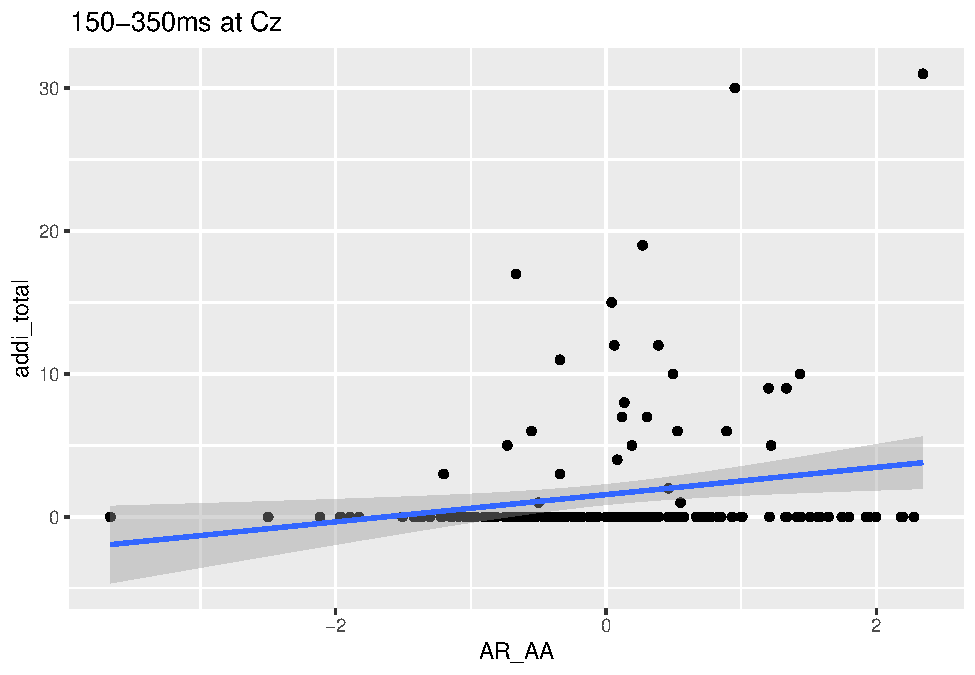
\includegraphics{do01_BUDS_files/figure-latex/unnamed-chunk-28-1.pdf}

\begin{Shaded}
\begin{Highlighting}[]
\FunctionTok{ggplot}\NormalTok{(df\_150350\_cz }\SpecialCharTok{\%\textgreater{}\%} \FunctionTok{filter}\NormalTok{(df\_150350\_cz}\SpecialCharTok{$}\NormalTok{addi\_total}\SpecialCharTok{\textless{}}\DecValTok{20}\NormalTok{), }\FunctionTok{aes}\NormalTok{(}\AttributeTok{x=}\NormalTok{AA\_AR, }\AttributeTok{y=}\NormalTok{addi\_total)) }\SpecialCharTok{+}
  \FunctionTok{geom\_point}\NormalTok{() }\SpecialCharTok{+}
  \FunctionTok{stat\_smooth}\NormalTok{(}\AttributeTok{method=}\StringTok{"lm"}\NormalTok{) }\SpecialCharTok{+}
  \FunctionTok{labs}\NormalTok{(}\AttributeTok{title=}\StringTok{"150{-}350ms at Cz"}\NormalTok{)}
\end{Highlighting}
\end{Shaded}

\includegraphics{do01_BUDS_files/figure-latex/unnamed-chunk-28-2.pdf}

\begin{Shaded}
\begin{Highlighting}[]
\FunctionTok{summary}\NormalTok{(}\FunctionTok{zeroinfl}\NormalTok{(}\AttributeTok{formula =}\NormalTok{ addi\_distress }\SpecialCharTok{\textasciitilde{}}\NormalTok{ AR\_AA, }\AttributeTok{data =}\NormalTok{ df\_200400\_pz))}
\FunctionTok{ggplot}\NormalTok{(df\_200400\_pz, }\FunctionTok{aes}\NormalTok{(}\AttributeTok{x=}\NormalTok{AR\_AA, }\AttributeTok{y=}\NormalTok{addi\_distress)) }\SpecialCharTok{+}
  \FunctionTok{geom\_point}\NormalTok{() }\SpecialCharTok{+}
  \FunctionTok{stat\_smooth}\NormalTok{(}\AttributeTok{method=}\StringTok{"lm"}\NormalTok{) }\SpecialCharTok{+}
  \FunctionTok{labs}\NormalTok{(}\AttributeTok{title=}\StringTok{"200{-}400ms at Pz"}\NormalTok{)}
\end{Highlighting}
\end{Shaded}

\begin{verbatim}
## Warning: Removed 28 rows containing non-finite values (`stat_smooth()`).
## Removed 28 rows containing missing values (`geom_point()`).
\end{verbatim}

\includegraphics{do01_BUDS_files/figure-latex/unnamed-chunk-28-3.pdf}

\begin{Shaded}
\begin{Highlighting}[]
\FunctionTok{ggplot}\NormalTok{(df\_200400\_pz }\SpecialCharTok{\%\textgreater{}\%} \FunctionTok{filter}\NormalTok{(df\_200400\_pz}\SpecialCharTok{$}\NormalTok{addi\_distress}\SpecialCharTok{\textless{}}\DecValTok{15}\NormalTok{), }\FunctionTok{aes}\NormalTok{(}\AttributeTok{x=}\NormalTok{AA\_AR, }\AttributeTok{y=}\NormalTok{addi\_distress)) }\SpecialCharTok{+}
  \FunctionTok{geom\_point}\NormalTok{() }\SpecialCharTok{+}
  \FunctionTok{stat\_smooth}\NormalTok{(}\AttributeTok{method=}\StringTok{"lm"}\NormalTok{) }\SpecialCharTok{+}
  \FunctionTok{labs}\NormalTok{(}\AttributeTok{title=}\StringTok{"200{-}400ms at Pz"}\NormalTok{)}
\end{Highlighting}
\end{Shaded}

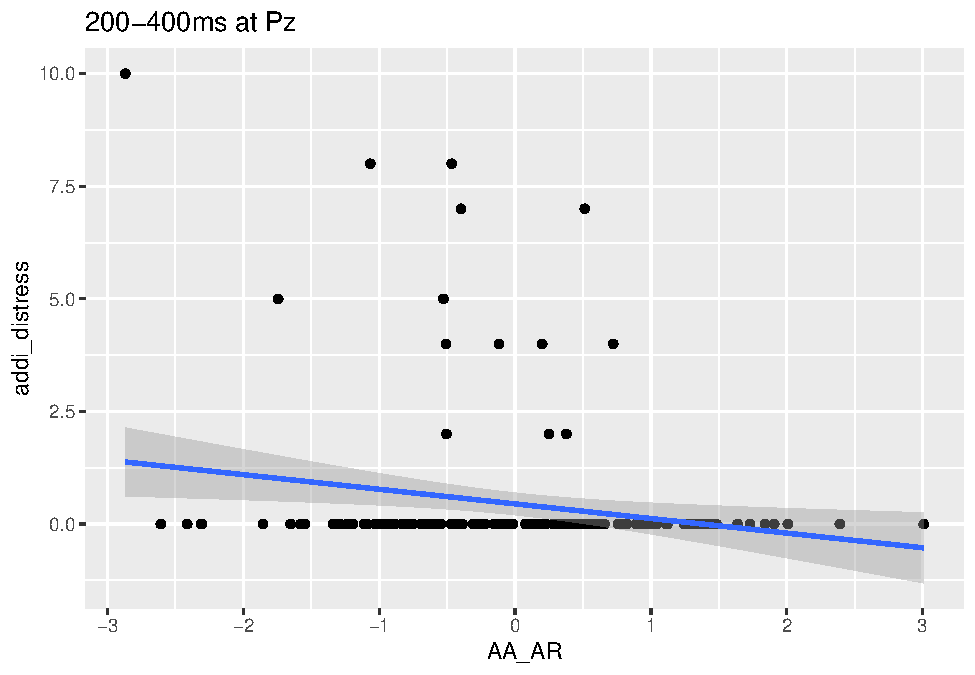
\includegraphics{do01_BUDS_files/figure-latex/unnamed-chunk-28-4.pdf}

\hypertarget{regressions-with-bcs-a}{%
\section{Regressions with BCS-A}\label{regressions-with-bcs-a}}

\begin{Shaded}
\begin{Highlighting}[]
\ControlFlowTok{for}\NormalTok{ (p }\ControlFlowTok{in} \FunctionTok{c}\NormalTok{(}\StringTok{"bcs\_physical\_vic"}\NormalTok{,}\StringTok{"bcs\_physical\_vic\_01"}\NormalTok{,}\StringTok{"bcs\_verbal\_vic"}\NormalTok{,}\StringTok{"bcs\_rel\_vic"}\NormalTok{,}\StringTok{"bcs\_cyber\_vic"}\NormalTok{,}\StringTok{"bcs\_total\_vic"}\NormalTok{)) \{}
      \FunctionTok{eval}\NormalTok{(}\FunctionTok{parse}\NormalTok{(}\AttributeTok{text=}\FunctionTok{paste0}\NormalTok{(}\StringTok{\textquotesingle{}hist(\textquotesingle{}}\NormalTok{,data,}\StringTok{\textquotesingle{}$\textquotesingle{}}\NormalTok{,p,}\StringTok{\textquotesingle{})\textquotesingle{}}\NormalTok{)))}
\NormalTok{    \}}

\ControlFlowTok{for}\NormalTok{ (data }\ControlFlowTok{in} \FunctionTok{c}\NormalTok{(}\StringTok{"df\_150350\_cz"}\NormalTok{,}\StringTok{"df\_250450\_fz"}\NormalTok{,}\StringTok{"df\_200400\_pz"}\NormalTok{)) \{}
  \ControlFlowTok{for}\NormalTok{ (comp }\ControlFlowTok{in} \FunctionTok{c}\NormalTok{(}\StringTok{"A\_all"}\NormalTok{)) \{}
    \ControlFlowTok{for}\NormalTok{ (p }\ControlFlowTok{in} \FunctionTok{c}\NormalTok{(}\StringTok{"bcs\_physical\_vic"}\NormalTok{,}\StringTok{"bcs\_physical\_vic\_01"}\NormalTok{,}\StringTok{"bcs\_verbal\_vic"}\NormalTok{,}\StringTok{"bcs\_rel\_vic"}\NormalTok{,}\StringTok{"bcs\_cyber\_vic"}\NormalTok{,}\StringTok{"bcs\_total\_vic"}\NormalTok{)) \{}
      \FunctionTok{eval}\NormalTok{(}\FunctionTok{parse}\NormalTok{(}\AttributeTok{text=}\FunctionTok{paste0}\NormalTok{(}\StringTok{\textquotesingle{}print(zeroinfl(\textquotesingle{}}\NormalTok{,p,}\StringTok{\textquotesingle{} \textasciitilde{} \textquotesingle{}}\NormalTok{,comp,}\StringTok{\textquotesingle{}, \textquotesingle{}}\NormalTok{,data,}\StringTok{\textquotesingle{})$call)}
\StringTok{                             print(round(summary(zeroinfl(\textquotesingle{}}\NormalTok{,p,}\StringTok{\textquotesingle{} \textasciitilde{} \textquotesingle{}}\NormalTok{,comp,}\StringTok{\textquotesingle{}, \textquotesingle{}}\NormalTok{,data,}\StringTok{\textquotesingle{}))$coefficients$count,3))\textquotesingle{}}\NormalTok{)))}
\NormalTok{    \}\}\}}


\ControlFlowTok{for}\NormalTok{ (data }\ControlFlowTok{in} \FunctionTok{c}\NormalTok{(}\StringTok{"df\_150350\_cz"}\NormalTok{)) \{}
  \ControlFlowTok{for}\NormalTok{ (comp }\ControlFlowTok{in} \FunctionTok{c}\NormalTok{(}\StringTok{"RA\_RR"}\NormalTok{)) \{}
    \ControlFlowTok{for}\NormalTok{ (p }\ControlFlowTok{in} \FunctionTok{c}\NormalTok{(}\StringTok{"bcs\_physical\_vic"}\NormalTok{,}\StringTok{"bcs\_physical\_vic\_01"}\NormalTok{,}\StringTok{"bcs\_verbal\_vic"}\NormalTok{,}\StringTok{"bcs\_rel\_vic"}\NormalTok{,}\StringTok{"bcs\_cyber\_vic"}\NormalTok{,}\StringTok{"bcs\_total\_vic"}\NormalTok{)) \{}
      \FunctionTok{eval}\NormalTok{(}\FunctionTok{parse}\NormalTok{(}\AttributeTok{text=}\FunctionTok{paste0}\NormalTok{(}\StringTok{\textquotesingle{}print(zeroinfl(\textquotesingle{}}\NormalTok{,p,}\StringTok{\textquotesingle{} \textasciitilde{} \textquotesingle{}}\NormalTok{,comp,}\StringTok{\textquotesingle{}, \textquotesingle{}}\NormalTok{,data,}\StringTok{\textquotesingle{})$call)}
\StringTok{                             print(round(summary(zeroinfl(\textquotesingle{}}\NormalTok{,p,}\StringTok{\textquotesingle{} \textasciitilde{} \textquotesingle{}}\NormalTok{,comp,}\StringTok{\textquotesingle{}, \textquotesingle{}}\NormalTok{,data,}\StringTok{\textquotesingle{}))$coefficients$count,3))\textquotesingle{}}\NormalTok{)))}
\NormalTok{    \}\}\}}

\ControlFlowTok{for}\NormalTok{ (data }\ControlFlowTok{in} \FunctionTok{c}\NormalTok{(}\StringTok{"df\_250450\_fz"}\NormalTok{)) \{}
  \ControlFlowTok{for}\NormalTok{ (comp }\ControlFlowTok{in} \FunctionTok{c}\NormalTok{(}\StringTok{"AA\_AR"}\NormalTok{)) \{}
   \ControlFlowTok{for}\NormalTok{ (p }\ControlFlowTok{in} \FunctionTok{c}\NormalTok{(}\StringTok{"bcs\_physical\_vic"}\NormalTok{,}\StringTok{"bcs\_physical\_vic\_01"}\NormalTok{,}\StringTok{"bcs\_verbal\_vic"}\NormalTok{,}\StringTok{"bcs\_rel\_vic"}\NormalTok{,}\StringTok{"bcs\_cyber\_vic"}\NormalTok{,}\StringTok{"bcs\_total\_vic"}\NormalTok{)) \{}
      \FunctionTok{eval}\NormalTok{(}\FunctionTok{parse}\NormalTok{(}\AttributeTok{text=}\FunctionTok{paste0}\NormalTok{(}\StringTok{\textquotesingle{}print(zeroinfl(\textquotesingle{}}\NormalTok{,p,}\StringTok{\textquotesingle{} \textasciitilde{} \textquotesingle{}}\NormalTok{,comp,}\StringTok{\textquotesingle{}, \textquotesingle{}}\NormalTok{,data,}\StringTok{\textquotesingle{})$call)}
\StringTok{                             print(round(summary(zeroinfl(\textquotesingle{}}\NormalTok{,p,}\StringTok{\textquotesingle{} \textasciitilde{} \textquotesingle{}}\NormalTok{,comp,}\StringTok{\textquotesingle{}, \textquotesingle{}}\NormalTok{,data,}\StringTok{\textquotesingle{}))$coefficients$count,3))\textquotesingle{}}\NormalTok{)))}
\NormalTok{   \}\}\}}

\ControlFlowTok{for}\NormalTok{ (data }\ControlFlowTok{in} \FunctionTok{c}\NormalTok{(}\StringTok{"df\_200400\_pz"}\NormalTok{)) \{}
  \ControlFlowTok{for}\NormalTok{ (comp }\ControlFlowTok{in} \FunctionTok{c}\NormalTok{(}\StringTok{"AR\_RR"}\NormalTok{,}\StringTok{"RA\_RR"}\NormalTok{,}\StringTok{"RA\_AA"}\NormalTok{)) \{}
    \ControlFlowTok{for}\NormalTok{ (p }\ControlFlowTok{in} \FunctionTok{c}\NormalTok{(}\StringTok{"bcs\_physical\_vic"}\NormalTok{,}\StringTok{"bcs\_physical\_vic\_01"}\NormalTok{,}\StringTok{"bcs\_verbal\_vic"}\NormalTok{,}\StringTok{"bcs\_rel\_vic"}\NormalTok{,}\StringTok{"bcs\_cyber\_vic"}\NormalTok{,}\StringTok{"bcs\_total\_vic"}\NormalTok{)) \{}
      \FunctionTok{eval}\NormalTok{(}\FunctionTok{parse}\NormalTok{(}\AttributeTok{text=}\FunctionTok{paste0}\NormalTok{(}\StringTok{\textquotesingle{}print(zeroinfl(\textquotesingle{}}\NormalTok{,p,}\StringTok{\textquotesingle{} \textasciitilde{} \textquotesingle{}}\NormalTok{,comp,}\StringTok{\textquotesingle{}, \textquotesingle{}}\NormalTok{,data,}\StringTok{\textquotesingle{})$call)}
\StringTok{                             print(round(summary(zeroinfl(\textquotesingle{}}\NormalTok{,p,}\StringTok{\textquotesingle{} \textasciitilde{} \textquotesingle{}}\NormalTok{,comp,}\StringTok{\textquotesingle{}, \textquotesingle{}}\NormalTok{,data,}\StringTok{\textquotesingle{}))$coefficients$count,3))\textquotesingle{}}\NormalTok{)))}
\NormalTok{    \}\}\}}

\CommentTok{\# for (data in c("df\_4001000\_pz")) \{}
\CommentTok{\#   for (comp in c("RR\_RA","AA\_RA")) \{}
\CommentTok{\#     for (p in c("bcs\_physical\_vic","bcs\_physical\_vic\_01","bcs\_verbal\_vic","bcs\_rel\_vic","bcs\_cyber\_vic","bcs\_total\_vic")) \{}
\CommentTok{\#       eval(parse(text=paste0(\textquotesingle{}print(zeroinfl(\textquotesingle{},p,\textquotesingle{} \textasciitilde{} \textquotesingle{},comp,\textquotesingle{}, \textquotesingle{},data,\textquotesingle{})$call)}
\CommentTok{\#                              print(round(summary(zeroinfl(\textquotesingle{},p,\textquotesingle{} \textasciitilde{} \textquotesingle{},comp,\textquotesingle{}, \textquotesingle{},data,\textquotesingle{}))$coefficients$count,3))\textquotesingle{})))}
\CommentTok{\#     }\RegionMarkerTok{\}\}\}}
\end{Highlighting}
\end{Shaded}

\hypertarget{no-significant-results}{%
\subsection{No significant results}\label{no-significant-results}}

\hypertarget{regressions-with-promis}{%
\section{Regressions with PROMIS}\label{regressions-with-promis}}

\begin{Shaded}
\begin{Highlighting}[]
\ControlFlowTok{for}\NormalTok{ (p }\ControlFlowTok{in} \FunctionTok{c}\NormalTok{(}\StringTok{"promis\_peer\_sumraw"}\NormalTok{,}\StringTok{"promis\_fam\_sumraw"}\NormalTok{,}\StringTok{"promis\_peer\_tscore"}\NormalTok{,}\StringTok{"promis\_fam\_tscore"}\NormalTok{)) \{}
      \FunctionTok{eval}\NormalTok{(}\FunctionTok{parse}\NormalTok{(}\AttributeTok{text=}\FunctionTok{paste0}\NormalTok{(}\StringTok{\textquotesingle{}hist(\textquotesingle{}}\NormalTok{,data,}\StringTok{\textquotesingle{}$\textquotesingle{}}\NormalTok{,p,}\StringTok{\textquotesingle{})\textquotesingle{}}\NormalTok{)))}
\NormalTok{    \}}

\ControlFlowTok{for}\NormalTok{ (data }\ControlFlowTok{in} \FunctionTok{c}\NormalTok{(}\StringTok{"df\_150350\_cz"}\NormalTok{,}\StringTok{"df\_250450\_fz"}\NormalTok{,}\StringTok{"df\_200400\_pz"}\NormalTok{)) \{}
  \ControlFlowTok{for}\NormalTok{ (comp }\ControlFlowTok{in} \FunctionTok{c}\NormalTok{(}\StringTok{"A\_all"}\NormalTok{)) \{}
    \ControlFlowTok{for}\NormalTok{ (p }\ControlFlowTok{in} \FunctionTok{c}\NormalTok{(}\StringTok{"promis\_peer\_sumraw"}\NormalTok{,}\StringTok{"promis\_fam\_sumraw"}\NormalTok{,}\StringTok{"promis\_peer\_tscore"}\NormalTok{,}\StringTok{"promis\_fam\_tscore"}\NormalTok{)) \{}
      \FunctionTok{eval}\NormalTok{(}\FunctionTok{parse}\NormalTok{(}\AttributeTok{text=}\FunctionTok{paste0}\NormalTok{(}\StringTok{\textquotesingle{}print(summary(lm(\textquotesingle{}}\NormalTok{,comp,}\StringTok{\textquotesingle{} \textasciitilde{} \textquotesingle{}}\NormalTok{,p,}\StringTok{\textquotesingle{}, \textquotesingle{}}\NormalTok{,data,}\StringTok{\textquotesingle{}))$coefficients)\textquotesingle{}}\NormalTok{)))}
\NormalTok{    \}\}\}}

\ControlFlowTok{for}\NormalTok{ (data }\ControlFlowTok{in} \FunctionTok{c}\NormalTok{(}\StringTok{"df\_150350\_cz"}\NormalTok{,}\StringTok{"df\_250450\_fz"}\NormalTok{,}\StringTok{"df\_200400\_pz"}\NormalTok{)) \{}
  \ControlFlowTok{for}\NormalTok{ (comp }\ControlFlowTok{in} \FunctionTok{c}\NormalTok{(}\StringTok{"A\_all"}\NormalTok{)) \{}
    \ControlFlowTok{for}\NormalTok{ (p }\ControlFlowTok{in} \FunctionTok{c}\NormalTok{(}\StringTok{"promis\_peer\_sumraw"}\NormalTok{,}\StringTok{"promis\_fam\_sumraw"}\NormalTok{,}\StringTok{"promis\_peer\_tscore"}\NormalTok{,}\StringTok{"promis\_fam\_tscore"}\NormalTok{)) \{}
      \FunctionTok{eval}\NormalTok{(}\FunctionTok{parse}\NormalTok{(}\AttributeTok{text=}\FunctionTok{paste0}\NormalTok{(}\StringTok{\textquotesingle{}print(summary(lm(\textquotesingle{}}\NormalTok{,comp,}\StringTok{\textquotesingle{} \textasciitilde{} \textquotesingle{}}\NormalTok{,p,}\StringTok{\textquotesingle{}, \textquotesingle{}}\NormalTok{,data,}\StringTok{\textquotesingle{}))$coefficients)\textquotesingle{}}\NormalTok{)))}
\NormalTok{\}\}\}}

\ControlFlowTok{for}\NormalTok{ (data }\ControlFlowTok{in} \FunctionTok{c}\NormalTok{(}\StringTok{"df\_150350\_cz"}\NormalTok{)) \{}
  \ControlFlowTok{for}\NormalTok{ (comp }\ControlFlowTok{in} \FunctionTok{c}\NormalTok{(}\StringTok{"RA\_RR"}\NormalTok{)) \{}
    \ControlFlowTok{for}\NormalTok{ (p }\ControlFlowTok{in} \FunctionTok{c}\NormalTok{(}\StringTok{"promis\_peer\_sumraw"}\NormalTok{,}\StringTok{"promis\_fam\_sumraw"}\NormalTok{,}\StringTok{"promis\_peer\_tscore"}\NormalTok{,}\StringTok{"promis\_fam\_tscore"}\NormalTok{)) \{}
      \FunctionTok{eval}\NormalTok{(}\FunctionTok{parse}\NormalTok{(}\AttributeTok{text=}\FunctionTok{paste0}\NormalTok{(}\StringTok{\textquotesingle{}print(summary(lm(\textquotesingle{}}\NormalTok{,comp,}\StringTok{\textquotesingle{} \textasciitilde{} \textquotesingle{}}\NormalTok{,p,}\StringTok{\textquotesingle{}, \textquotesingle{}}\NormalTok{,data,}\StringTok{\textquotesingle{}))$coefficients)\textquotesingle{}}\NormalTok{)))}
\NormalTok{\}\}\}}

\ControlFlowTok{for}\NormalTok{ (data }\ControlFlowTok{in} \FunctionTok{c}\NormalTok{(}\StringTok{"df\_250450\_fz"}\NormalTok{)) \{}
  \ControlFlowTok{for}\NormalTok{ (comp }\ControlFlowTok{in} \FunctionTok{c}\NormalTok{(}\StringTok{"AA\_AR"}\NormalTok{)) \{}
    \ControlFlowTok{for}\NormalTok{ (p }\ControlFlowTok{in} \FunctionTok{c}\NormalTok{(}\StringTok{"promis\_peer\_sumraw"}\NormalTok{,}\StringTok{"promis\_fam\_sumraw"}\NormalTok{,}\StringTok{"promis\_peer\_tscore"}\NormalTok{,}\StringTok{"promis\_fam\_tscore"}\NormalTok{)) \{}
      \FunctionTok{eval}\NormalTok{(}\FunctionTok{parse}\NormalTok{(}\AttributeTok{text=}\FunctionTok{paste0}\NormalTok{(}\StringTok{\textquotesingle{}print(summary(lm(\textquotesingle{}}\NormalTok{,comp,}\StringTok{\textquotesingle{} \textasciitilde{} \textquotesingle{}}\NormalTok{,p,}\StringTok{\textquotesingle{}, \textquotesingle{}}\NormalTok{,data,}\StringTok{\textquotesingle{}))$coefficients)\textquotesingle{}}\NormalTok{)))}
\NormalTok{\}\}\}}

\ControlFlowTok{for}\NormalTok{ (data }\ControlFlowTok{in} \FunctionTok{c}\NormalTok{(}\StringTok{"df\_200400\_pz"}\NormalTok{)) \{}
  \ControlFlowTok{for}\NormalTok{ (comp }\ControlFlowTok{in} \FunctionTok{c}\NormalTok{(}\StringTok{"AR\_RR"}\NormalTok{,}\StringTok{"RA\_RR"}\NormalTok{,}\StringTok{"RA\_AA"}\NormalTok{)) \{}
    \ControlFlowTok{for}\NormalTok{ (p }\ControlFlowTok{in} \FunctionTok{c}\NormalTok{(}\StringTok{"promis\_peer\_sumraw"}\NormalTok{,}\StringTok{"promis\_fam\_sumraw"}\NormalTok{,}\StringTok{"promis\_peer\_tscore"}\NormalTok{,}\StringTok{"promis\_fam\_tscore"}\NormalTok{)) \{}
      \FunctionTok{eval}\NormalTok{(}\FunctionTok{parse}\NormalTok{(}\AttributeTok{text=}\FunctionTok{paste0}\NormalTok{(}\StringTok{\textquotesingle{}print(summary(lm(\textquotesingle{}}\NormalTok{,comp,}\StringTok{\textquotesingle{} \textasciitilde{} \textquotesingle{}}\NormalTok{,p,}\StringTok{\textquotesingle{}, \textquotesingle{}}\NormalTok{,data,}\StringTok{\textquotesingle{}))$coefficients)\textquotesingle{}}\NormalTok{)))}
\NormalTok{    \}\}\}}

\CommentTok{\# for (data in c("df\_4001000\_pz")) \{}
\CommentTok{\#   for (comp in c("RR\_RA","AA\_RA")) \{}
\CommentTok{\#     for (p in c("promis\_peer\_sumraw","promis\_fam\_sumraw","promis\_peer\_tscore","promis\_fam\_tscore")) \{}
\CommentTok{\#       eval(parse(text=paste0(\textquotesingle{}print(summary(lm(\textquotesingle{},comp,\textquotesingle{} \textasciitilde{} \textquotesingle{},p,\textquotesingle{}, \textquotesingle{},data,\textquotesingle{}))$coefficients)\textquotesingle{})))}
\CommentTok{\#     }\RegionMarkerTok{\}\}\}}
\end{Highlighting}
\end{Shaded}

\hypertarget{no-significant-results-1}{%
\subsection{No significant results}\label{no-significant-results-1}}

\hypertarget{regressions-with-romantic-relationship}{%
\section{Regressions with romantic
relationship}\label{regressions-with-romantic-relationship}}

\begin{Shaded}
\begin{Highlighting}[]
\FunctionTok{load}\NormalTok{(}\FunctionTok{here}\NormalTok{(}\StringTok{"data/BUDS\_cleaning02\_with\_strain.RData"}\NormalTok{))}
\NormalTok{BUDS\_cleaning02\_with\_strain}\SpecialCharTok{$}\NormalTok{ID }\OtherTok{\textless{}{-}} \FunctionTok{as.integer}\NormalTok{(}\FunctionTok{as.character}\NormalTok{(BUDS\_cleaning02\_with\_strain}\SpecialCharTok{$}\NormalTok{id\_1\_i))}
\NormalTok{BUDS\_cleaning02\_with\_strain }\OtherTok{\textless{}{-}}\NormalTok{ BUDS\_cleaning02\_with\_strain }\SpecialCharTok{\%\textgreater{}\%}
  \FunctionTok{distinct}\NormalTok{(ID, }\AttributeTok{.keep\_all=}\ConstantTok{TRUE}\NormalTok{) }\SpecialCharTok{\%\textgreater{}\%}
  \FunctionTok{mutate}\NormalTok{(}\AttributeTok{RelationshipStatus\_named =} \FunctionTok{case\_match}\NormalTok{(RelationshipStatus, }\DecValTok{1} \SpecialCharTok{\textasciitilde{}} \StringTok{"I\textquotesingle{}ve never had a boyfriend or girlfriend"}\NormalTok{,}
                                        \DecValTok{2} \SpecialCharTok{\textasciitilde{}} \StringTok{"I\textquotesingle{}ve had a boyfriend or girlfriend, but I\textquotesingle{}m not dating anyone right now"}\NormalTok{,}
                                        \DecValTok{3} \SpecialCharTok{\textasciitilde{}} \StringTok{"I\textquotesingle{}m dating someone, but it\textquotesingle{}s not very serious"}\NormalTok{,}
                                        \DecValTok{4} \SpecialCharTok{\textasciitilde{}} \StringTok{"I have a serious boyfriend or girlfriend"}\NormalTok{,}
                                        \DecValTok{5} \SpecialCharTok{\textasciitilde{}} \StringTok{"I am married"}\NormalTok{),}
         \AttributeTok{Never\_dated =} \FunctionTok{case\_when}\NormalTok{(RelationshipStatus }\SpecialCharTok{==} \DecValTok{1} \SpecialCharTok{\textasciitilde{}} \StringTok{"never\_dated"}\NormalTok{,}
\NormalTok{                                  RelationshipStatus }\SpecialCharTok{\textgreater{}} \DecValTok{1} \SpecialCharTok{\&}\NormalTok{  RelationshipStatus}\SpecialCharTok{!=}\DecValTok{2} \SpecialCharTok{\textasciitilde{}} \StringTok{"dated"}\NormalTok{),}
         \AttributeTok{RelationshipStatus\_named\_no4 =} \FunctionTok{case\_match}\NormalTok{(RelationshipStatus, }\DecValTok{1} \SpecialCharTok{\textasciitilde{}} \StringTok{"I\textquotesingle{}ve never had a boyfriend or girlfriend"}\NormalTok{,}
                                        \DecValTok{2} \SpecialCharTok{\textasciitilde{}} \StringTok{"I\textquotesingle{}ve had a boyfriend or girlfriend, but I\textquotesingle{}m not dating anyone right now"}\NormalTok{,}
                                        \DecValTok{3} \SpecialCharTok{\textasciitilde{}} \StringTok{"I\textquotesingle{}m dating someone, but it\textquotesingle{}s not very serious"}\NormalTok{,}
                                        \DecValTok{4} \SpecialCharTok{\textasciitilde{}} \ConstantTok{NA}\NormalTok{,}
                                        \DecValTok{5} \SpecialCharTok{\textasciitilde{}} \StringTok{"I am married"}\NormalTok{),}
         \AttributeTok{RelationshipStatus\_named\_no2 =} \FunctionTok{case\_match}\NormalTok{(RelationshipStatus, }\DecValTok{1} \SpecialCharTok{\textasciitilde{}} \StringTok{"I\textquotesingle{}ve never had a boyfriend or girlfriend"}\NormalTok{,}
                                        \DecValTok{2} \SpecialCharTok{\textasciitilde{}} \ConstantTok{NA}\NormalTok{,}
                                        \DecValTok{3} \SpecialCharTok{\textasciitilde{}} \StringTok{"I\textquotesingle{}m dating someone, but it\textquotesingle{}s not very serious"}\NormalTok{,}
                                        \DecValTok{4} \SpecialCharTok{\textasciitilde{}} \StringTok{"I have a serious boyfriend or girlfriend"}\NormalTok{,}
                                        \DecValTok{5} \SpecialCharTok{\textasciitilde{}} \StringTok{"I am married"}\NormalTok{))}



\NormalTok{df\_150350\_cz\_strain }\OtherTok{\textless{}{-}}\NormalTok{ df\_150350\_cz }\SpecialCharTok{\%\textgreater{}\%}
  \FunctionTok{full\_join}\NormalTok{(BUDS\_cleaning02\_with\_strain, }\AttributeTok{by=}\StringTok{"ID"}\NormalTok{)}
  
\NormalTok{df\_250450\_fz\_strain }\OtherTok{\textless{}{-}}\NormalTok{ df\_250450\_fz }\SpecialCharTok{\%\textgreater{}\%}
  \FunctionTok{full\_join}\NormalTok{(BUDS\_cleaning02\_with\_strain, }\AttributeTok{by=}\StringTok{"ID"}\NormalTok{)}

\NormalTok{df\_200400\_pz\_strain }\OtherTok{\textless{}{-}}\NormalTok{ df\_200400\_pz }\SpecialCharTok{\%\textgreater{}\%}
  \FunctionTok{full\_join}\NormalTok{(BUDS\_cleaning02\_with\_strain, }\AttributeTok{by=}\StringTok{"ID"}\NormalTok{)}

\CommentTok{\# df\_4001000\_pz\_strain \textless{}{-} df\_4001000\_pz \%\textgreater{}\%}
\CommentTok{\#   full\_join(BUDS\_cleaning02\_with\_strain, by="ID")}
\CommentTok{\# }
\CommentTok{\# df\_6001500\_pz\_strain \textless{}{-} df\_6001500\_pz \%\textgreater{}\%}
\CommentTok{\#   full\_join(BUDS\_cleaning02\_with\_strain, by="ID")}

\FunctionTok{table}\NormalTok{(df\_150350\_cz\_strain}\SpecialCharTok{$}\NormalTok{RelationshipStatus\_named)}
\FunctionTok{table}\NormalTok{(df\_150350\_cz\_strain}\SpecialCharTok{$}\NormalTok{Never\_dated)}

\CommentTok{\# Acceptance from a liked peer relative to acceptance from a disliked peer is greater for youth who have never dated than for youth who have dated}
\CommentTok{\# summary(lm(AA\_RA \textasciitilde{} Never\_dated, data = df\_4001000\_pz\_strain))}
\CommentTok{\# summary(lm(A\_all \textasciitilde{} Never\_dated, data = df\_4001000\_pz\_strain))}

\CommentTok{\# ggplot(filter(df\_4001000\_pz\_strain, complete.cases(Never\_dated)), aes(y=A\_all, x=Never\_dated)) +}
  \CommentTok{\# geom\_bar(stat="summary", position = "dodge", fun.y = "mean")}

\CommentTok{\# df\_4001000\_pz\_hcs\_strain \textless{}{-} df\_4001000\_pz\_hcs \%\textgreater{}\%}
  \CommentTok{\# full\_join(BUDS\_cleaning02\_with\_strain, by="ID")}
\CommentTok{\# anova(lm(call = AA\_RA \textasciitilde{} Never\_dated, data = df\_4001000\_pz\_hcs\_strain))}

\CommentTok{\# t.test(A\_all \textasciitilde{} Never\_dated, df\_4001000\_pz\_strain)}
\CommentTok{\# t.test(AA\_RA \textasciitilde{} Never\_dated, df\_4001000\_pz\_hcs\_strain)}

\CommentTok{\# for (data in c("df\_200400\_pz\_strain")) \{}
\CommentTok{\#   for (comp in c("AR\_RR","RA\_RR","RA\_AA")) \{}
\CommentTok{\#     for (p in c("RelationshipStatus","Never\_dated")) \{}
\CommentTok{\#       eval(parse(text=paste0(\textquotesingle{}print(summary(lm(\textquotesingle{},comp,\textquotesingle{} \textasciitilde{} \textquotesingle{},p,\textquotesingle{}, \textquotesingle{},data,\textquotesingle{})))\textquotesingle{})))}
\CommentTok{\#     }\RegionMarkerTok{\}\}\}}
\end{Highlighting}
\end{Shaded}

\begin{Shaded}
\begin{Highlighting}[]
\NormalTok{df\_4001000\_pz\_strain\_idas }\OtherTok{\textless{}{-}}\NormalTok{ df\_4001000\_pz\_strain}

\ControlFlowTok{for}\NormalTok{ (var }\ControlFlowTok{in} \FunctionTok{c}\NormalTok{(}\DecValTok{15}\NormalTok{,}\DecValTok{18}\NormalTok{,}\DecValTok{20}\NormalTok{,}\DecValTok{41}\NormalTok{,}\DecValTok{47}\NormalTok{,}\DecValTok{99}\NormalTok{,}
              \DecValTok{3}\NormalTok{,}\DecValTok{10}\NormalTok{,}\DecValTok{23}\NormalTok{,}\DecValTok{27}\NormalTok{,}\DecValTok{50}\NormalTok{,}\DecValTok{53}\NormalTok{,}\DecValTok{59}\NormalTok{,}\DecValTok{64}\NormalTok{)) \{}
 \FunctionTok{eval}\NormalTok{(}\FunctionTok{parse}\NormalTok{(}\AttributeTok{text=}\FunctionTok{paste0}\NormalTok{(}\StringTok{\textquotesingle{}}
\StringTok{  df\_4001000\_pz\_strain\_idas$idas\_\textquotesingle{}}\NormalTok{,var,}\StringTok{\textquotesingle{} \textless{}{-} dplyr::recode\_factor(df\_4001000\_pz\_strain\_idas$idas\_\textquotesingle{}}\NormalTok{,var,}\StringTok{\textquotesingle{}\_i.y, }
\StringTok{  "Not at all"=1, }
\StringTok{  "A little bit"=2, }
\StringTok{  "Moderately"=3,}
\StringTok{  "Quite a bit"=4,}
\StringTok{  "Extremely"=5, }
\StringTok{  \textasciigrave{}1\textasciigrave{}=1, \textasciigrave{}2\textasciigrave{}=2, \textasciigrave{}3\textasciigrave{}=3, \textasciigrave{}4\textasciigrave{}=4,\textasciigrave{}5\textasciigrave{}=5)}
\StringTok{  df\_4001000\_pz\_strain\_idas$idas\_\textquotesingle{}}\NormalTok{,var,}\StringTok{\textquotesingle{} \textless{}{-} as.integer(df\_4001000\_pz\_strain\_idas$idas\_\textquotesingle{}}\NormalTok{,var,}\StringTok{\textquotesingle{})\textquotesingle{}}\NormalTok{)))}
\NormalTok{\}}

\ControlFlowTok{for}\NormalTok{ (var }\ControlFlowTok{in} \FunctionTok{c}\NormalTok{(}\DecValTok{1}\SpecialCharTok{:}\DecValTok{17}\NormalTok{)) \{}
 \FunctionTok{eval}\NormalTok{(}\FunctionTok{parse}\NormalTok{(}\AttributeTok{text=}\FunctionTok{paste0}\NormalTok{(}\StringTok{\textquotesingle{}}
\StringTok{  df\_4001000\_pz\_strain\_idas$acips\_\textquotesingle{}}\NormalTok{,var,}\StringTok{\textquotesingle{} \textless{}{-} dplyr::recode\_factor(df\_4001000\_pz\_strain\_idas$acips\_\textquotesingle{}}\NormalTok{,var,}\StringTok{\textquotesingle{}\_i.y, }
\StringTok{  "Very false for me"=1, }
\StringTok{  "Moderately false for me"=2, }
\StringTok{  "Slightly false for me"=3,}
\StringTok{  "Slightly true for me"=4,}
\StringTok{  "Moderately true for me"=5, }
\StringTok{  "Very true for me"=6,}
\StringTok{  \textasciigrave{}1\textasciigrave{}=1, \textasciigrave{}2\textasciigrave{}=2, \textasciigrave{}3\textasciigrave{}=3, \textasciigrave{}4\textasciigrave{}=4,\textasciigrave{}5\textasciigrave{}=5, \textasciigrave{}6\textasciigrave{}=6)}
\StringTok{  df\_4001000\_pz\_strain\_idas$acips\_\textquotesingle{}}\NormalTok{,var,}\StringTok{\textquotesingle{} \textless{}{-} as.integer(df\_4001000\_pz\_strain\_idas$acips\_\textquotesingle{}}\NormalTok{,var,}\StringTok{\textquotesingle{})\textquotesingle{}}\NormalTok{)))}
\NormalTok{\}}

\NormalTok{df\_4001000\_pz\_strain\_idas}\SpecialCharTok{$}\NormalTok{idas\_sa }\OtherTok{\textless{}{-}} \FunctionTok{rowMeans}\NormalTok{(df\_4001000\_pz\_strain\_idas[,}\FunctionTok{c}\NormalTok{(}\StringTok{"idas\_15"}\NormalTok{,}\StringTok{"idas\_18"}\NormalTok{,}
                                                                        \StringTok{"idas\_20"}\NormalTok{,}\StringTok{"idas\_41"}\NormalTok{,}
                                                                        \StringTok{"idas\_47"}\NormalTok{,}\StringTok{"idas\_99"}\NormalTok{)], }\AttributeTok{na.rm=}\NormalTok{T)}
\NormalTok{df\_4001000\_pz\_strain\_idas}\SpecialCharTok{$}\NormalTok{idas\_wellbeing }\OtherTok{\textless{}{-}} \FunctionTok{rowMeans}\NormalTok{(df\_4001000\_pz\_strain\_idas[,}\FunctionTok{c}\NormalTok{(}\StringTok{"idas\_3"}\NormalTok{,}\StringTok{"idas\_10"}\NormalTok{,}
                                                                        \StringTok{"idas\_23"}\NormalTok{,}\StringTok{"idas\_27"}\NormalTok{,}
                                                                        \StringTok{"idas\_50"}\NormalTok{,}\StringTok{"idas\_53"}\NormalTok{,}
                                                                        \StringTok{"idas\_59"}\NormalTok{,}\StringTok{"idas\_64"}\NormalTok{)], }\AttributeTok{na.rm=}\NormalTok{T)}
\NormalTok{df\_4001000\_pz\_strain\_idas}\SpecialCharTok{$}\NormalTok{acips }\OtherTok{\textless{}{-}} \FunctionTok{rowMeans}\NormalTok{(df\_4001000\_pz\_strain\_idas[,}\FunctionTok{c}\NormalTok{(}\StringTok{"acips\_1"}\NormalTok{,}\StringTok{"acips\_2"}\NormalTok{,}
                                                                        \StringTok{"acips\_3"}\NormalTok{,}\StringTok{"acips\_4"}\NormalTok{,}
                                                                        \StringTok{"acips\_5"}\NormalTok{,}\StringTok{"acips\_6"}\NormalTok{,}
                                                                       \StringTok{"acips\_7"}\NormalTok{,}\StringTok{"acips\_8"}\NormalTok{,}
                                                                       \StringTok{"acips\_9"}\NormalTok{,}\StringTok{"acips\_10"}\NormalTok{,}
                                                                       \StringTok{"acips\_11"}\NormalTok{,}\StringTok{"acips\_12"}\NormalTok{,}
                                                                       \StringTok{"acips\_13"}\NormalTok{,}\StringTok{"acips\_14"}\NormalTok{,}
                                                                       \StringTok{"acips\_15"}\NormalTok{,}\StringTok{"acips\_16"}\NormalTok{,}\StringTok{"acips\_17"}\NormalTok{)], }\AttributeTok{na.rm=}\NormalTok{T)}

\NormalTok{df\_4001000\_pz\_strain\_idas}\SpecialCharTok{$}\NormalTok{idas\_sa\_norm }\OtherTok{\textless{}{-}} \FunctionTok{bestNormalize}\NormalTok{(df\_4001000\_pz\_strain\_idas}\SpecialCharTok{$}\NormalTok{idas\_sa)}\SpecialCharTok{$}\NormalTok{x.t}
\FunctionTok{hist}\NormalTok{(df\_4001000\_pz\_strain\_idas}\SpecialCharTok{$}\NormalTok{idas\_sa\_norm)}

\NormalTok{df\_4001000\_pz\_strain\_idas}\SpecialCharTok{$}\NormalTok{acips\_norm }\OtherTok{\textless{}{-}} \FunctionTok{bestNormalize}\NormalTok{(df\_4001000\_pz\_strain\_idas}\SpecialCharTok{$}\NormalTok{acips)}\SpecialCharTok{$}\NormalTok{x.t}
\FunctionTok{hist}\NormalTok{(df\_4001000\_pz\_strain\_idas}\SpecialCharTok{$}\NormalTok{acips\_norm)}

\FunctionTok{t.test}\NormalTok{(idas\_sa\_norm }\SpecialCharTok{\textasciitilde{}}\NormalTok{ Never\_dated, df\_4001000\_pz\_strain\_idas)}
\FunctionTok{t.test}\NormalTok{(idas\_wellbeing }\SpecialCharTok{\textasciitilde{}}\NormalTok{ Never\_dated, df\_4001000\_pz\_strain\_idas)}
\FunctionTok{t.test}\NormalTok{(acips }\SpecialCharTok{\textasciitilde{}}\NormalTok{ Never\_dated, df\_4001000\_pz\_strain\_idas)}

\FunctionTok{summary}\NormalTok{(}\FunctionTok{lm}\NormalTok{(AA\_RA }\SpecialCharTok{\textasciitilde{}}\NormalTok{ idas\_sa\_norm }\SpecialCharTok{+}\NormalTok{ acips\_norm }\SpecialCharTok{+}\NormalTok{ idas\_wellbeing, df\_4001000\_pz\_strain\_idas))}
\FunctionTok{summary}\NormalTok{(}\FunctionTok{lm}\NormalTok{(AA\_RA }\SpecialCharTok{\textasciitilde{}}\NormalTok{ idas\_sa\_norm}\SpecialCharTok{*}\NormalTok{Never\_dated, df\_4001000\_pz\_strain\_idas))}

\CommentTok{\# SEND THIS TO STEW}
\FunctionTok{summary}\NormalTok{(}\FunctionTok{lm}\NormalTok{(AA\_AR }\SpecialCharTok{\textasciitilde{}}\NormalTok{ idas\_sa\_norm }\SpecialCharTok{+}\NormalTok{ idas\_wellbeing, df\_4001000\_pz\_strain\_idas))}

\NormalTok{df\_4001000\_pz\_strain\_idas\_complete }\OtherTok{\textless{}{-}}\NormalTok{ df\_4001000\_pz\_strain\_idas }\SpecialCharTok{\%\textgreater{}\%}
  \FunctionTok{filter}\NormalTok{(}\FunctionTok{complete.cases}\NormalTok{(AA\_AR) }\SpecialCharTok{\&} \FunctionTok{complete.cases}\NormalTok{(idas\_sa\_norm) }\SpecialCharTok{\&} \FunctionTok{complete.cases}\NormalTok{(idas\_wellbeing))}

\NormalTok{fit}\FloatTok{.1} \OtherTok{\textless{}{-}} \FunctionTok{lm}\NormalTok{(AA\_AR }\SpecialCharTok{\textasciitilde{}}\NormalTok{ idas\_sa\_norm, }\AttributeTok{data=}\NormalTok{df\_4001000\_pz\_strain\_idas\_complete)}
\NormalTok{fit}\FloatTok{.2} \OtherTok{\textless{}{-}} \FunctionTok{lm}\NormalTok{(AA\_AR }\SpecialCharTok{\textasciitilde{}}\NormalTok{ idas\_wellbeing, }\AttributeTok{data=}\NormalTok{df\_4001000\_pz\_strain\_idas\_complete)}
\NormalTok{df\_4001000\_pz\_strain\_idas\_complete}\SpecialCharTok{$}\NormalTok{residual2 }\OtherTok{\textless{}{-}} \FunctionTok{residuals}\NormalTok{(fit}\FloatTok{.2}\NormalTok{)}
\NormalTok{df\_4001000\_pz\_strain\_idas\_complete}\SpecialCharTok{$}\NormalTok{residual1 }\OtherTok{\textless{}{-}} \FunctionTok{residuals}\NormalTok{(}\FunctionTok{lm}\NormalTok{(idas\_sa\_norm }\SpecialCharTok{\textasciitilde{}}\NormalTok{ idas\_wellbeing, df\_4001000\_pz\_strain\_idas\_complete))}

\CommentTok{\# Check and make sure these lead to the same effect as the regular multiple regression model}
\FunctionTok{round}\NormalTok{(}\FunctionTok{summary}\NormalTok{(}\FunctionTok{lm}\NormalTok{(AA\_AR }\SpecialCharTok{\textasciitilde{}}\NormalTok{ idas\_sa\_norm }\SpecialCharTok{+}\NormalTok{ idas\_wellbeing, df\_4001000\_pz\_strain\_idas))}\SpecialCharTok{$}\NormalTok{coefficients[}\DecValTok{2}\NormalTok{,],}\DecValTok{3}\NormalTok{)}
\FunctionTok{round}\NormalTok{(}\FunctionTok{summary}\NormalTok{(}\FunctionTok{lm}\NormalTok{(residual2 }\SpecialCharTok{\textasciitilde{}}\NormalTok{ residual1, df\_4001000\_pz\_strain\_idas\_complete))}\SpecialCharTok{$}\NormalTok{coefficients[}\DecValTok{2}\NormalTok{,],}\DecValTok{3}\NormalTok{)}
\CommentTok{\# yea, these are basically the same except for some slight change due to rounding and the fact that the first model has 1 more df than the second, multiple regression model}

\FunctionTok{ggplot}\NormalTok{(df\_4001000\_pz\_strain\_idas\_complete, }\FunctionTok{aes}\NormalTok{(}\AttributeTok{x=}\NormalTok{residual1, }\AttributeTok{y=}\NormalTok{residual2)) }\SpecialCharTok{+}
  \FunctionTok{geom\_point}\NormalTok{() }\SpecialCharTok{+}
  \FunctionTok{stat\_smooth}\NormalTok{(}\AttributeTok{method=}\StringTok{"lm"}\NormalTok{, }\AttributeTok{color=}\StringTok{"black"}\NormalTok{, }\AttributeTok{se=}\ConstantTok{TRUE}\NormalTok{) }\SpecialCharTok{+}
  \FunctionTok{labs}\NormalTok{(}\AttributeTok{x=}\StringTok{"Social anxiety symptoms"}\NormalTok{, }\AttributeTok{y=}\StringTok{"Response to high{-}value peer acceptance"}\NormalTok{) }\SpecialCharTok{+}
\NormalTok{  papaja}\SpecialCharTok{::}\FunctionTok{theme\_apa}\NormalTok{() }\SpecialCharTok{+}
  \FunctionTok{theme}\NormalTok{(}\AttributeTok{text =} \FunctionTok{element\_text}\NormalTok{(}\AttributeTok{size =} \DecValTok{16}\NormalTok{))   }

\FunctionTok{ggplot}\NormalTok{(df\_4001000\_pz\_strain\_idas\_complete, }\FunctionTok{aes}\NormalTok{(}\AttributeTok{x=}\NormalTok{idas\_sa\_norm, }\AttributeTok{y=}\NormalTok{AA\_AR)) }\SpecialCharTok{+}
  \FunctionTok{geom\_point}\NormalTok{() }\SpecialCharTok{+}
  \FunctionTok{stat\_smooth}\NormalTok{(}\AttributeTok{method=}\StringTok{"lm"}\NormalTok{) }\SpecialCharTok{+}
\NormalTok{    papaja}\SpecialCharTok{::}\FunctionTok{theme\_apa}\NormalTok{()}
\end{Highlighting}
\end{Shaded}

\hypertarget{regressions-with-strain}{%
\section{Regressions with STRAIN}\label{regressions-with-strain}}

\hypertarget{all-stressors}{%
\subsection{All stressors}\label{all-stressors}}

\begin{Shaded}
\begin{Highlighting}[]
\NormalTok{stressors }\OtherTok{\textless{}{-}} \FunctionTok{c}\NormalTok{(}\StringTok{"StressCT"}\NormalTok{,}\StringTok{"StressTH"}\NormalTok{,}\StringTok{"EvntCT"}\NormalTok{,}\StringTok{"DiffCT"}\NormalTok{,}\StringTok{"EvntTH"}\NormalTok{,}\StringTok{"DiffTH"}\NormalTok{)}

\CommentTok{\# RewP, P3, LPP}
\ControlFlowTok{for}\NormalTok{ (data }\ControlFlowTok{in} \FunctionTok{c}\NormalTok{(}\StringTok{"df\_150350\_cz\_strain"}\NormalTok{,}\StringTok{"df\_250450\_fz\_strain"}\NormalTok{,}\StringTok{"df\_200400\_pz\_strain"}\NormalTok{,}
               \StringTok{"df\_4001000\_pz\_strain"}\NormalTok{,}\StringTok{"df\_6001500\_pz\_strain"}\NormalTok{)) \{}
  \ControlFlowTok{for}\NormalTok{ (comp }\ControlFlowTok{in} \FunctionTok{c}\NormalTok{(}\StringTok{"A\_all"}\NormalTok{,}\StringTok{"AA\_AR"}\NormalTok{,}\StringTok{"RA\_RR"}\NormalTok{)) \{}
    \ControlFlowTok{for}\NormalTok{ (p }\ControlFlowTok{in}\NormalTok{ stressors) \{}
      \FunctionTok{eval}\NormalTok{(}\FunctionTok{parse}\NormalTok{(}\AttributeTok{text=}\FunctionTok{paste0}\NormalTok{(}\StringTok{\textquotesingle{}print(summary(lm(\textquotesingle{}}\NormalTok{,comp,}\StringTok{\textquotesingle{} \textasciitilde{} \textquotesingle{}}\NormalTok{,p,}\StringTok{\textquotesingle{}, \textquotesingle{}}\NormalTok{,data,}\StringTok{\textquotesingle{}))$coef[2,4])\textquotesingle{}}\NormalTok{)))}
\NormalTok{    \}\}\}}


\CommentTok{\# LPP}
\ControlFlowTok{for}\NormalTok{ (data }\ControlFlowTok{in} \FunctionTok{c}\NormalTok{(}\StringTok{"df\_4001000\_pz\_strain"}\NormalTok{,}\StringTok{"df\_6001500\_pz\_strain"}\NormalTok{)) \{}
  \ControlFlowTok{for}\NormalTok{ (comp }\ControlFlowTok{in} \FunctionTok{c}\NormalTok{(}\StringTok{"RR\_RA"}\NormalTok{,}\StringTok{"AA\_RA"}\NormalTok{)) \{}
    \ControlFlowTok{for}\NormalTok{ (p }\ControlFlowTok{in}\NormalTok{ stressors) \{}
      \FunctionTok{eval}\NormalTok{(}\FunctionTok{parse}\NormalTok{(}\AttributeTok{text=}\FunctionTok{paste0}\NormalTok{(}\StringTok{\textquotesingle{}print(summary(lm(\textquotesingle{}}\NormalTok{,comp,}\StringTok{\textquotesingle{} \textasciitilde{} \textquotesingle{}}\NormalTok{,p,}\StringTok{\textquotesingle{}, \textquotesingle{}}\NormalTok{,data,}\StringTok{\textquotesingle{}))$coef[2,4])\textquotesingle{}}\NormalTok{)))}
\NormalTok{    \}\}\}}

\CommentTok{\# P3}
\ControlFlowTok{for}\NormalTok{ (data }\ControlFlowTok{in} \FunctionTok{c}\NormalTok{(}\StringTok{"df\_200400\_pz\_strain"}\NormalTok{)) \{}
  \ControlFlowTok{for}\NormalTok{ (comp }\ControlFlowTok{in} \FunctionTok{c}\NormalTok{(}\StringTok{"AR\_RR"}\NormalTok{,}\StringTok{"RA\_AA"}\NormalTok{)) \{}
    \ControlFlowTok{for}\NormalTok{ (p }\ControlFlowTok{in}\NormalTok{ stressors) \{}
      \FunctionTok{eval}\NormalTok{(}\FunctionTok{parse}\NormalTok{(}\AttributeTok{text=}\FunctionTok{paste0}\NormalTok{(}\StringTok{\textquotesingle{}print(summary(lm(\textquotesingle{}}\NormalTok{,comp,}\StringTok{\textquotesingle{} \textasciitilde{} \textquotesingle{}}\NormalTok{,p,}\StringTok{\textquotesingle{}, \textquotesingle{}}\NormalTok{,data,}\StringTok{\textquotesingle{}))$coef[2,4])\textquotesingle{}}\NormalTok{)))}
\NormalTok{    \}\}\}}
\end{Highlighting}
\end{Shaded}

\hypertarget{interpersonal-loss}{%
\subsection{Interpersonal Loss}\label{interpersonal-loss}}

\begin{Shaded}
\begin{Highlighting}[]
\NormalTok{interpersonal\_loss }\OtherTok{\textless{}{-}} \FunctionTok{c}\NormalTok{(}\StringTok{"CIEvntCT"}\NormalTok{,}\StringTok{"CIDiffCT"}\NormalTok{,}\StringTok{"CIAllCT"}\NormalTok{,}\StringTok{"CIEvntTH"}\NormalTok{,}\StringTok{"CIDiffTH"}\NormalTok{,}\StringTok{"CIAllTH"}\NormalTok{)}

\CommentTok{\# RewP, P3, LPP}
\ControlFlowTok{for}\NormalTok{ (data }\ControlFlowTok{in} \FunctionTok{c}\NormalTok{(}\StringTok{"df\_150350\_cz\_strain"}\NormalTok{,}\StringTok{"df\_250450\_fz\_strain"}\NormalTok{,}\StringTok{"df\_200400\_pz\_strain"}\NormalTok{,}
               \StringTok{"df\_4001000\_pz\_strain"}\NormalTok{,}\StringTok{"df\_6001500\_pz\_strain"}\NormalTok{)) \{}
  \ControlFlowTok{for}\NormalTok{ (comp }\ControlFlowTok{in} \FunctionTok{c}\NormalTok{(}\StringTok{"A\_all"}\NormalTok{,}\StringTok{"AA\_AR"}\NormalTok{,}\StringTok{"RA\_RR"}\NormalTok{)) \{}
    \ControlFlowTok{for}\NormalTok{ (p }\ControlFlowTok{in}\NormalTok{ interpersonal\_loss) \{}
      \FunctionTok{eval}\NormalTok{(}\FunctionTok{parse}\NormalTok{(}\AttributeTok{text=}\FunctionTok{paste0}\NormalTok{(}\StringTok{\textquotesingle{}print(summary(lm(\textquotesingle{}}\NormalTok{,comp,}\StringTok{\textquotesingle{} \textasciitilde{} \textquotesingle{}}\NormalTok{,p,}\StringTok{\textquotesingle{}, \textquotesingle{}}\NormalTok{,data,}\StringTok{\textquotesingle{}))$coef[2,4])\textquotesingle{}}\NormalTok{)))}
\NormalTok{    \}\}\}}


\CommentTok{\# LPP}
\ControlFlowTok{for}\NormalTok{ (data }\ControlFlowTok{in} \FunctionTok{c}\NormalTok{(}\StringTok{"df\_4001000\_pz\_strain"}\NormalTok{,}\StringTok{"df\_6001500\_pz\_strain"}\NormalTok{)) \{}
  \ControlFlowTok{for}\NormalTok{ (comp }\ControlFlowTok{in} \FunctionTok{c}\NormalTok{(}\StringTok{"RR\_RA"}\NormalTok{,}\StringTok{"AA\_RA"}\NormalTok{)) \{}
    \ControlFlowTok{for}\NormalTok{ (p }\ControlFlowTok{in}\NormalTok{ interpersonal\_loss) \{}
      \FunctionTok{eval}\NormalTok{(}\FunctionTok{parse}\NormalTok{(}\AttributeTok{text=}\FunctionTok{paste0}\NormalTok{(}\StringTok{\textquotesingle{}print(summary(lm(\textquotesingle{}}\NormalTok{,comp,}\StringTok{\textquotesingle{} \textasciitilde{} \textquotesingle{}}\NormalTok{,p,}\StringTok{\textquotesingle{}, \textquotesingle{}}\NormalTok{,data,}\StringTok{\textquotesingle{}))$coef[2,4])\textquotesingle{}}\NormalTok{)))}
\NormalTok{    \}\}\}}

\CommentTok{\# P3}
\ControlFlowTok{for}\NormalTok{ (data }\ControlFlowTok{in} \FunctionTok{c}\NormalTok{(}\StringTok{"df\_200400\_pz\_strain"}\NormalTok{)) \{}
  \ControlFlowTok{for}\NormalTok{ (comp }\ControlFlowTok{in} \FunctionTok{c}\NormalTok{(}\StringTok{"AR\_RR"}\NormalTok{,}\StringTok{"RA\_AA"}\NormalTok{)) \{}
    \ControlFlowTok{for}\NormalTok{ (p }\ControlFlowTok{in}\NormalTok{ interpersonal\_loss) \{}
      \FunctionTok{eval}\NormalTok{(}\FunctionTok{parse}\NormalTok{(}\AttributeTok{text=}\FunctionTok{paste0}\NormalTok{(}\StringTok{\textquotesingle{}print(summary(lm(\textquotesingle{}}\NormalTok{,comp,}\StringTok{\textquotesingle{} \textasciitilde{} \textquotesingle{}}\NormalTok{,p,}\StringTok{\textquotesingle{}, \textquotesingle{}}\NormalTok{,data,}\StringTok{\textquotesingle{}))$coef[2,4])\textquotesingle{}}\NormalTok{)))}
\NormalTok{    \}\}\}}
\end{Highlighting}
\end{Shaded}

\hypertarget{humiliation}{%
\subsection{Humiliation}\label{humiliation}}

\hypertarget{full-sample}{%
\subsubsection{Full sample}\label{full-sample}}

\begin{Shaded}
\begin{Highlighting}[]
\NormalTok{humiliation }\OtherTok{\textless{}{-}} \FunctionTok{c}\NormalTok{(}\StringTok{"CHEvntCT"}\NormalTok{,}\StringTok{"CHDiffCT"}\NormalTok{,}\StringTok{"CHAllCT"}\NormalTok{,}\StringTok{"CHEvntTH"}\NormalTok{,}\StringTok{"CHDiffTH"}\NormalTok{,}\StringTok{"CHAllTH"}\NormalTok{)}

\CommentTok{\# RewP, P3, LPP}
\ControlFlowTok{for}\NormalTok{ (data }\ControlFlowTok{in} \FunctionTok{c}\NormalTok{(}\StringTok{"df\_150350\_cz\_strain"}\NormalTok{,}\StringTok{"df\_250450\_fz\_strain"}\NormalTok{,}\StringTok{"df\_200400\_pz\_strain"}\NormalTok{,}
               \StringTok{"df\_4001000\_pz\_strain"}\NormalTok{,}\StringTok{"df\_6001500\_pz\_strain"}\NormalTok{)) \{}
  \ControlFlowTok{for}\NormalTok{ (comp }\ControlFlowTok{in} \FunctionTok{c}\NormalTok{(}\StringTok{"A\_all"}\NormalTok{,}\StringTok{"AA\_AR"}\NormalTok{,}\StringTok{"RA\_RR"}\NormalTok{)) \{}
    \ControlFlowTok{for}\NormalTok{ (p }\ControlFlowTok{in}\NormalTok{ humiliation) \{}
      \FunctionTok{eval}\NormalTok{(}\FunctionTok{parse}\NormalTok{(}\AttributeTok{text=}\FunctionTok{paste0}\NormalTok{(}\StringTok{\textquotesingle{}print(summary(lm(\textquotesingle{}}\NormalTok{,comp,}\StringTok{\textquotesingle{} \textasciitilde{} \textquotesingle{}}\NormalTok{,p,}\StringTok{\textquotesingle{}, \textquotesingle{}}\NormalTok{,data,}\StringTok{\textquotesingle{}))$coef[2,4])\textquotesingle{}}\NormalTok{)))}
\NormalTok{    \}\}\}}

\CommentTok{\# LPP}
\ControlFlowTok{for}\NormalTok{ (data }\ControlFlowTok{in} \FunctionTok{c}\NormalTok{(}\StringTok{"df\_4001000\_pz\_strain"}\NormalTok{,}\StringTok{"df\_6001500\_pz\_strain"}\NormalTok{)) \{}
  \ControlFlowTok{for}\NormalTok{ (comp }\ControlFlowTok{in} \FunctionTok{c}\NormalTok{(}\StringTok{"RR\_RA"}\NormalTok{,}\StringTok{"AA\_RA"}\NormalTok{)) \{}
    \ControlFlowTok{for}\NormalTok{ (p }\ControlFlowTok{in}\NormalTok{ humiliation) \{}
      \FunctionTok{eval}\NormalTok{(}\FunctionTok{parse}\NormalTok{(}\AttributeTok{text=}\FunctionTok{paste0}\NormalTok{(}\StringTok{\textquotesingle{}print(summary(lm(\textquotesingle{}}\NormalTok{,comp,}\StringTok{\textquotesingle{} \textasciitilde{} \textquotesingle{}}\NormalTok{,p,}\StringTok{\textquotesingle{}, \textquotesingle{}}\NormalTok{,data,}\StringTok{\textquotesingle{}))$coef[2,4])\textquotesingle{}}\NormalTok{)))}
\NormalTok{    \}\}\}}

\CommentTok{\# P3}
\ControlFlowTok{for}\NormalTok{ (data }\ControlFlowTok{in} \FunctionTok{c}\NormalTok{(}\StringTok{"df\_200400\_pz\_strain"}\NormalTok{)) \{}
  \ControlFlowTok{for}\NormalTok{ (comp }\ControlFlowTok{in} \FunctionTok{c}\NormalTok{(}\StringTok{"AR\_RR"}\NormalTok{,}\StringTok{"RA\_AA"}\NormalTok{)) \{}
    \ControlFlowTok{for}\NormalTok{ (p }\ControlFlowTok{in}\NormalTok{ humiliation) \{}
      \FunctionTok{eval}\NormalTok{(}\FunctionTok{parse}\NormalTok{(}\AttributeTok{text=}\FunctionTok{paste0}\NormalTok{(}\StringTok{\textquotesingle{}print(summary(lm(\textquotesingle{}}\NormalTok{,comp,}\StringTok{\textquotesingle{} \textasciitilde{} \textquotesingle{}}\NormalTok{,p,}\StringTok{\textquotesingle{}, \textquotesingle{}}\NormalTok{,data,}\StringTok{\textquotesingle{}))$coef[2,4])\textquotesingle{}}\NormalTok{)))}
\NormalTok{    \}\}\}}

\DocumentationTok{\#\#\#\#\#\#\#\#\#\#\#\#\#\#\#\#\#\#\#\#\#\#\#\#\#\#\#\#\#\#\#\#\#\#\#\#\#\#\#\#\#\#\#\#\#\#\#\#\#\#\#\#\#\#}

\ControlFlowTok{for}\NormalTok{ (data }\ControlFlowTok{in} \FunctionTok{c}\NormalTok{(}\StringTok{"df\_250450\_fz\_strain"}\NormalTok{)) \{}
  \ControlFlowTok{for}\NormalTok{ (comp }\ControlFlowTok{in} \FunctionTok{c}\NormalTok{(}\StringTok{"AA\_AR"}\NormalTok{)) \{}
    \ControlFlowTok{for}\NormalTok{ (p }\ControlFlowTok{in}\NormalTok{ humiliation) \{}
      \FunctionTok{eval}\NormalTok{(}\FunctionTok{parse}\NormalTok{(}\AttributeTok{text=}\FunctionTok{paste0}\NormalTok{(}\StringTok{\textquotesingle{}print(summary(lm(\textquotesingle{}}\NormalTok{,comp,}\StringTok{\textquotesingle{} \textasciitilde{} \textquotesingle{}}\NormalTok{,p,}\StringTok{\textquotesingle{}, \textquotesingle{}}\NormalTok{,data,}\StringTok{\textquotesingle{})))\textquotesingle{}}\NormalTok{)))}
\NormalTok{    \}\}\}}

\FunctionTok{summary}\NormalTok{(}\FunctionTok{lm}\NormalTok{(}\AttributeTok{formula =}\NormalTok{ AA\_AR }\SpecialCharTok{\textasciitilde{}}\NormalTok{ CHAllCT, }\AttributeTok{data =}\NormalTok{ df\_250450\_fz\_strain)) }\CommentTok{\#Characteristic: Humiliation {-} Total Count}
\FunctionTok{summary}\NormalTok{(}\FunctionTok{lm}\NormalTok{(}\AttributeTok{formula =}\NormalTok{ AA\_AR }\SpecialCharTok{\textasciitilde{}}\NormalTok{ CHAllTH, }\AttributeTok{data =}\NormalTok{ df\_250450\_fz\_strain)) }\CommentTok{\#Characteristic: Humiliation {-} Total Severity}
\FunctionTok{summary}\NormalTok{(}\FunctionTok{lm}\NormalTok{(}\AttributeTok{formula =}\NormalTok{ AA\_AR }\SpecialCharTok{\textasciitilde{}}\NormalTok{ CHEvntCT, }\AttributeTok{data =}\NormalTok{ df\_250450\_fz\_strain)) }\CommentTok{\#Characteristic: Humiliation {-} Count of Acute Life Events}
\FunctionTok{summary}\NormalTok{(}\FunctionTok{lm}\NormalTok{(}\AttributeTok{formula =}\NormalTok{ AA\_AR }\SpecialCharTok{\textasciitilde{}}\NormalTok{ CHEvntTH, }\AttributeTok{data =}\NormalTok{ df\_250450\_fz\_strain)) }\CommentTok{\#\textasciitilde{} Characteristic: Humiliation {-} Severity of Acute Life Events }

\FunctionTok{ggplot}\NormalTok{(df\_250450\_fz\_strain, }\FunctionTok{aes}\NormalTok{(}\AttributeTok{x=}\NormalTok{CHAllCT, }\AttributeTok{y=}\NormalTok{AA\_AR)) }\SpecialCharTok{+}
  \FunctionTok{geom\_point}\NormalTok{() }\SpecialCharTok{+}
  \FunctionTok{stat\_smooth}\NormalTok{(}\AttributeTok{method=}\StringTok{"lm"}\NormalTok{)}

\FunctionTok{ggplot}\NormalTok{(df\_250450\_fz\_strain, }\FunctionTok{aes}\NormalTok{(}\AttributeTok{x=}\NormalTok{CHAllTH, }\AttributeTok{y=}\NormalTok{AA\_AR)) }\SpecialCharTok{+}
  \FunctionTok{geom\_point}\NormalTok{() }\SpecialCharTok{+}
  \FunctionTok{stat\_smooth}\NormalTok{(}\AttributeTok{method=}\StringTok{"lm"}\NormalTok{)}
  
\FunctionTok{ggplot}\NormalTok{(df\_250450\_fz\_strain, }\FunctionTok{aes}\NormalTok{(}\AttributeTok{x=}\NormalTok{CHEvntCT, }\AttributeTok{y=}\NormalTok{AA\_AR)) }\SpecialCharTok{+}
  \FunctionTok{geom\_point}\NormalTok{() }\SpecialCharTok{+}
  \FunctionTok{stat\_smooth}\NormalTok{(}\AttributeTok{method=}\StringTok{"lm"}\NormalTok{)}
\end{Highlighting}
\end{Shaded}

These findings are specific to humiliation type stressors from the
STRAIN.

The direction suggests that greater experience with humiliating life
events is related to a enhanced response to acceptance relative to
rejection. However, since rejection appears to elicits a greater ERP
than rejection in this time window (i.e., negative difference), it is
more interpretable as greater experience with humiliating life events is
related to a less negative net response to rejection (right?).

\hypertarget{financial}{%
\subsection{Financial}\label{financial}}

\begin{Shaded}
\begin{Highlighting}[]
\NormalTok{financial }\OtherTok{\textless{}{-}} \FunctionTok{c}\NormalTok{(}\StringTok{"DFEvntCT"}\NormalTok{,}\StringTok{"DFDiffCT"}\NormalTok{,}\StringTok{"DFAllCT"}\NormalTok{,}\StringTok{"DFEvntTH"}\NormalTok{,}\StringTok{"DFDiffTH"}\NormalTok{,}\StringTok{"DFAllTH"}\NormalTok{)}

\ControlFlowTok{for}\NormalTok{ (p }\ControlFlowTok{in}\NormalTok{ financial) \{}
  \ControlFlowTok{for}\NormalTok{ (data }\ControlFlowTok{in} \FunctionTok{c}\NormalTok{(}\StringTok{"df\_150350\_cz\_strain"}\NormalTok{,}\StringTok{"df\_250450\_fz\_strain"}\NormalTok{,}\StringTok{"df\_200400\_pz\_strain"}\NormalTok{)) \{}
  \ControlFlowTok{for}\NormalTok{ (comp }\ControlFlowTok{in} \FunctionTok{c}\NormalTok{(}\StringTok{"RR\_RA"}\NormalTok{)) \{}
      \FunctionTok{eval}\NormalTok{(}\FunctionTok{parse}\NormalTok{(}\AttributeTok{text=}\FunctionTok{paste0}\NormalTok{(}\StringTok{\textquotesingle{}print(summary(lm(\textquotesingle{}}\NormalTok{,comp,}\StringTok{\textquotesingle{} \textasciitilde{} \textquotesingle{}}\NormalTok{,p,}\StringTok{\textquotesingle{}, \textquotesingle{}}\NormalTok{,data,}\StringTok{\textquotesingle{}))$call)}
\StringTok{                             print(summary(lm(\textquotesingle{}}\NormalTok{,comp,}\StringTok{\textquotesingle{} \textasciitilde{} \textquotesingle{}}\NormalTok{,p,}\StringTok{\textquotesingle{}, \textquotesingle{}}\NormalTok{,data,}\StringTok{\textquotesingle{}))$coef[2,4])\textquotesingle{}}\NormalTok{)))}
\NormalTok{    \}\}\}}



\FunctionTok{summary}\NormalTok{(}\FunctionTok{lm}\NormalTok{(}\AttributeTok{formula =}\NormalTok{ ADI\_NATRANK\_log\_z }\SpecialCharTok{\textasciitilde{}}\NormalTok{ DFDiffCT, }\AttributeTok{data =}\NormalTok{ df\_150350\_cz\_strain))}
\FunctionTok{summary}\NormalTok{(}\FunctionTok{lm}\NormalTok{(}\AttributeTok{formula =}\NormalTok{ ADI\_NATRANK\_log\_z }\SpecialCharTok{\textasciitilde{}}\NormalTok{ DFDiffTH, }\AttributeTok{data =}\NormalTok{ df\_150350\_cz\_strain))}

\CommentTok{\# Domain: Financial {-} Count of Chronic Difficulties}
\FunctionTok{summary}\NormalTok{(}\FunctionTok{lm}\NormalTok{(}\AttributeTok{formula =}\NormalTok{ DFDiffCT }\SpecialCharTok{\textasciitilde{}}\NormalTok{ RR\_RA, }\AttributeTok{data =}\NormalTok{ df\_150350\_cz\_strain))}
\FunctionTok{summary}\NormalTok{(}\FunctionTok{lm}\NormalTok{(}\AttributeTok{formula =}\NormalTok{ DFDiffCT }\SpecialCharTok{\textasciitilde{}}\NormalTok{ RR\_RA, }\AttributeTok{data =}\NormalTok{ df\_250450\_fz\_strain))}

\FunctionTok{summary}\NormalTok{(}\FunctionTok{lm}\NormalTok{(}\AttributeTok{formula =}\NormalTok{ RR\_RA }\SpecialCharTok{\textasciitilde{}}\NormalTok{ DFAllCT, }\AttributeTok{data =}\NormalTok{ df\_250450\_fz\_strain))}

\CommentTok{\# Domain: Financial {-} Severity of Chronic Difficulties}
\FunctionTok{summary}\NormalTok{(}\FunctionTok{lm}\NormalTok{(}\AttributeTok{formula =}\NormalTok{ RR\_RA }\SpecialCharTok{\textasciitilde{}}\NormalTok{ DFDiffTH, }\AttributeTok{data =}\NormalTok{ df\_150350\_cz\_strain))}
\FunctionTok{summary}\NormalTok{(}\FunctionTok{lm}\NormalTok{(}\AttributeTok{formula =}\NormalTok{ RR\_RA }\SpecialCharTok{\textasciitilde{}}\NormalTok{ DFDiffTH, }\AttributeTok{data =}\NormalTok{ df\_250450\_fz\_strain))}

\FunctionTok{summary}\NormalTok{(}\FunctionTok{lm}\NormalTok{(}\AttributeTok{formula =}\NormalTok{ RR\_RA }\SpecialCharTok{\textasciitilde{}}\NormalTok{ DFAllTH, }\AttributeTok{data =}\NormalTok{ df\_250450\_fz\_strain))}

\NormalTok{df\_150350\_cz\_strain}\SpecialCharTok{$}\NormalTok{DFDiffCT\_z }\OtherTok{\textless{}{-}} \FunctionTok{scale}\NormalTok{(df\_150350\_cz\_strain}\SpecialCharTok{$}\NormalTok{DFDiffCT, }\AttributeTok{scale=}\NormalTok{T, }\AttributeTok{center=}\NormalTok{T)}
\NormalTok{df\_150350\_cz\_strain}\SpecialCharTok{$}\NormalTok{DFDiffTH\_z }\OtherTok{\textless{}{-}} \FunctionTok{scale}\NormalTok{(df\_150350\_cz\_strain}\SpecialCharTok{$}\NormalTok{DFDiffTH, }\AttributeTok{scale=}\NormalTok{T, }\AttributeTok{center=}\NormalTok{T)}

\NormalTok{df\_250450\_fz\_strain}\SpecialCharTok{$}\NormalTok{DFDiffCT\_z }\OtherTok{\textless{}{-}} \FunctionTok{scale}\NormalTok{(df\_250450\_fz\_strain}\SpecialCharTok{$}\NormalTok{DFDiffCT, }\AttributeTok{scale=}\NormalTok{T, }\AttributeTok{center=}\NormalTok{T)}
\NormalTok{df\_250450\_fz\_strain}\SpecialCharTok{$}\NormalTok{DFDiffTH\_z }\OtherTok{\textless{}{-}} \FunctionTok{scale}\NormalTok{(df\_250450\_fz\_strain}\SpecialCharTok{$}\NormalTok{DFDiffTH, }\AttributeTok{scale=}\NormalTok{T, }\AttributeTok{center=}\NormalTok{T)}

\FunctionTok{ggplot}\NormalTok{(df\_150350\_cz\_strain, }\FunctionTok{aes}\NormalTok{(}\AttributeTok{x=}\NormalTok{DFDiffCT\_z, }\AttributeTok{y=}\NormalTok{RR\_RA)) }\SpecialCharTok{+}
  \FunctionTok{geom\_point}\NormalTok{() }\SpecialCharTok{+}
  \FunctionTok{stat\_smooth}\NormalTok{(}\AttributeTok{method=}\StringTok{"lm"}\NormalTok{) }\SpecialCharTok{+}
  \FunctionTok{geom\_text}\NormalTok{(}\AttributeTok{x=}\DecValTok{2}\NormalTok{, }\AttributeTok{y=}\SpecialCharTok{{-}}\FloatTok{2.5}\NormalTok{, }\AttributeTok{color=}\StringTok{"blue"}\NormalTok{, }\AttributeTok{size=}\DecValTok{5}\NormalTok{, }\AttributeTok{label=}\FunctionTok{paste0}\NormalTok{(}\StringTok{"beta="}\NormalTok{,}
       \FunctionTok{round}\NormalTok{(}\FunctionTok{tidy}\NormalTok{(}\FunctionTok{lm}\NormalTok{(}\AttributeTok{formula =}\NormalTok{ RR\_RA }\SpecialCharTok{\textasciitilde{}}\NormalTok{ DFDiffCT\_z, }\AttributeTok{data =}\NormalTok{ df\_150350\_cz\_strain))[}\DecValTok{2}\NormalTok{,}\FunctionTok{c}\NormalTok{(}\DecValTok{2}\NormalTok{)],}\DecValTok{3}\NormalTok{),}
       \StringTok{", p="}\NormalTok{, }
       \FunctionTok{round}\NormalTok{(}\FunctionTok{tidy}\NormalTok{(}\FunctionTok{lm}\NormalTok{(}\AttributeTok{formula =}\NormalTok{ RR\_RA }\SpecialCharTok{\textasciitilde{}}\NormalTok{ DFDiffCT\_z, }\AttributeTok{data =}\NormalTok{ df\_150350\_cz\_strain))[}\DecValTok{2}\NormalTok{,}\FunctionTok{c}\NormalTok{(}\DecValTok{5}\NormalTok{)],}\DecValTok{3}\NormalTok{))) }\SpecialCharTok{+}
    \FunctionTok{labs}\NormalTok{(}\AttributeTok{x=}\StringTok{"Low value rejection }\SpecialCharTok{\textbackslash{}n}\StringTok{(relative to low value acceptance)"}\NormalTok{,}
       \AttributeTok{y=}\StringTok{"STRAIN financial chronic stressors (count)"}\NormalTok{,}
       \AttributeTok{title=}\StringTok{"150{-}350 ms at Cz"}\NormalTok{)}

\FunctionTok{ggplot}\NormalTok{(df\_250450\_fz\_strain, }\FunctionTok{aes}\NormalTok{(}\AttributeTok{x=}\NormalTok{DFDiffCT\_z, }\AttributeTok{y=}\NormalTok{RR\_RA)) }\SpecialCharTok{+}
  \FunctionTok{geom\_point}\NormalTok{() }\SpecialCharTok{+}
  \FunctionTok{stat\_smooth}\NormalTok{(}\AttributeTok{method=}\StringTok{"lm"}\NormalTok{) }\SpecialCharTok{+}
  \FunctionTok{geom\_text}\NormalTok{(}\AttributeTok{x=}\DecValTok{3}\NormalTok{, }\AttributeTok{y=}\SpecialCharTok{{-}}\FloatTok{2.5}\NormalTok{, }\AttributeTok{color=}\StringTok{"blue"}\NormalTok{, }\AttributeTok{size=}\DecValTok{5}\NormalTok{, }\AttributeTok{label=}\FunctionTok{paste0}\NormalTok{(}\StringTok{"beta="}\NormalTok{,}
       \FunctionTok{round}\NormalTok{(}\FunctionTok{tidy}\NormalTok{(}\FunctionTok{lm}\NormalTok{(}\AttributeTok{formula =}\NormalTok{ RR\_RA }\SpecialCharTok{\textasciitilde{}}\NormalTok{ DFDiffCT\_z, }\AttributeTok{data =}\NormalTok{ df\_250450\_fz\_strain))[}\DecValTok{2}\NormalTok{,}\FunctionTok{c}\NormalTok{(}\DecValTok{2}\NormalTok{)],}\DecValTok{3}\NormalTok{),}
       \StringTok{", p="}\NormalTok{, }
       \FunctionTok{round}\NormalTok{(}\FunctionTok{tidy}\NormalTok{(}\FunctionTok{lm}\NormalTok{(}\AttributeTok{formula =}\NormalTok{ RR\_RA }\SpecialCharTok{\textasciitilde{}}\NormalTok{ DFDiffCT\_z, }\AttributeTok{data =}\NormalTok{ df\_250450\_fz\_strain))[}\DecValTok{2}\NormalTok{,}\FunctionTok{c}\NormalTok{(}\DecValTok{5}\NormalTok{)],}\DecValTok{3}\NormalTok{))) }\SpecialCharTok{+}
    \FunctionTok{labs}\NormalTok{(}\AttributeTok{x=}\StringTok{"Low value rejection }\SpecialCharTok{\textbackslash{}n}\StringTok{(relative to low value acceptance)"}\NormalTok{,}
       \AttributeTok{y=}\StringTok{"STRAIN financial chronic stressors (count)"}\NormalTok{,}
       \AttributeTok{title=}\StringTok{"250{-}450 ms at Fz"}\NormalTok{)}

\FunctionTok{ggplot}\NormalTok{(df\_150350\_cz\_strain, }\FunctionTok{aes}\NormalTok{(}\AttributeTok{x=}\NormalTok{DFDiffTH\_z, }\AttributeTok{y=}\NormalTok{RR\_RA)) }\SpecialCharTok{+}
  \FunctionTok{geom\_point}\NormalTok{() }\SpecialCharTok{+}
  \FunctionTok{stat\_smooth}\NormalTok{(}\AttributeTok{method=}\StringTok{"lm"}\NormalTok{) }\SpecialCharTok{+}
  \FunctionTok{geom\_text}\NormalTok{(}\AttributeTok{x=}\DecValTok{14}\NormalTok{, }\AttributeTok{y=}\SpecialCharTok{{-}}\FloatTok{2.5}\NormalTok{, }\AttributeTok{color=}\StringTok{"blue"}\NormalTok{, }\AttributeTok{size=}\DecValTok{5}\NormalTok{, }\AttributeTok{label=}\FunctionTok{paste0}\NormalTok{(}\StringTok{"beta="}\NormalTok{,}
       \FunctionTok{round}\NormalTok{(}\FunctionTok{tidy}\NormalTok{(}\FunctionTok{lm}\NormalTok{(}\AttributeTok{formula =}\NormalTok{ RR\_RA }\SpecialCharTok{\textasciitilde{}}\NormalTok{ DFDiffTH\_z, }\AttributeTok{data =}\NormalTok{ df\_150350\_cz\_strain))[}\DecValTok{2}\NormalTok{,}\FunctionTok{c}\NormalTok{(}\DecValTok{2}\NormalTok{)],}\DecValTok{3}\NormalTok{),}
       \StringTok{", p="}\NormalTok{, }
       \FunctionTok{round}\NormalTok{(}\FunctionTok{tidy}\NormalTok{(}\FunctionTok{lm}\NormalTok{(}\AttributeTok{formula =}\NormalTok{ RR\_RA }\SpecialCharTok{\textasciitilde{}}\NormalTok{ DFDiffTH\_z, }\AttributeTok{data =}\NormalTok{ df\_150350\_cz\_strain))[}\DecValTok{2}\NormalTok{,}\FunctionTok{c}\NormalTok{(}\DecValTok{5}\NormalTok{)],}\DecValTok{3}\NormalTok{))) }\SpecialCharTok{+}
    \FunctionTok{labs}\NormalTok{(}\AttributeTok{x=}\StringTok{"Low value rejection }\SpecialCharTok{\textbackslash{}n}\StringTok{(relative to low value acceptance)"}\NormalTok{,}
       \AttributeTok{y=}\StringTok{"STRAIN financial chronic stressors (severity)"}\NormalTok{,}
       \AttributeTok{title=}\StringTok{"150{-}350 ms at Cz"}\NormalTok{)}

\FunctionTok{ggplot}\NormalTok{(df\_250450\_fz\_strain, }\FunctionTok{aes}\NormalTok{(}\AttributeTok{x=}\NormalTok{DFDiffTH\_z, }\AttributeTok{y=}\NormalTok{RR\_RA)) }\SpecialCharTok{+}
  \FunctionTok{geom\_point}\NormalTok{() }\SpecialCharTok{+}
  \FunctionTok{stat\_smooth}\NormalTok{(}\AttributeTok{method=}\StringTok{"lm"}\NormalTok{) }\SpecialCharTok{+}
  \FunctionTok{geom\_text}\NormalTok{(}\AttributeTok{x=}\DecValTok{14}\NormalTok{, }\AttributeTok{y=}\SpecialCharTok{{-}}\DecValTok{3}\NormalTok{, }\AttributeTok{color=}\StringTok{"blue"}\NormalTok{, }\AttributeTok{size=}\DecValTok{5}\NormalTok{, }\AttributeTok{label=}\FunctionTok{paste0}\NormalTok{(}\StringTok{"beta="}\NormalTok{,}
       \FunctionTok{round}\NormalTok{(}\FunctionTok{tidy}\NormalTok{(}\FunctionTok{lm}\NormalTok{(}\AttributeTok{formula =}\NormalTok{ RR\_RA }\SpecialCharTok{\textasciitilde{}}\NormalTok{ DFDiffTH\_z, }\AttributeTok{data =}\NormalTok{ df\_250450\_fz\_strain))[}\DecValTok{2}\NormalTok{,}\FunctionTok{c}\NormalTok{(}\DecValTok{2}\NormalTok{)],}\DecValTok{3}\NormalTok{),}
       \StringTok{", p="}\NormalTok{, }
       \FunctionTok{round}\NormalTok{(}\FunctionTok{tidy}\NormalTok{(}\FunctionTok{lm}\NormalTok{(}\AttributeTok{formula =}\NormalTok{ RR\_RA }\SpecialCharTok{\textasciitilde{}}\NormalTok{ DFDiffTH\_z, }\AttributeTok{data =}\NormalTok{ df\_250450\_fz\_strain))[}\DecValTok{2}\NormalTok{,}\FunctionTok{c}\NormalTok{(}\DecValTok{5}\NormalTok{)],}\DecValTok{3}\NormalTok{))) }\SpecialCharTok{+}
    \FunctionTok{labs}\NormalTok{(}\AttributeTok{x=}\StringTok{"Low value rejection }\SpecialCharTok{\textbackslash{}n}\StringTok{(relative to low value acceptance)"}\NormalTok{,}
       \AttributeTok{y=}\StringTok{"STRAIN financial chronic stressors (severity)"}\NormalTok{,}
       \AttributeTok{title=}\StringTok{"250{-}450 ms at Fz"}\NormalTok{)}
\end{Highlighting}
\end{Shaded}

\begin{Shaded}
\begin{Highlighting}[]
\CommentTok{\# save(BUDS\_cleaning04, file=here("data/BUDS\_cleaning04.RData"))}
\end{Highlighting}
\end{Shaded}


\end{document}
